\documentclass{acm_proc_article-sp}
\usepackage[colorlinks,linkcolor=red,anchorcolor=blue,citecolor=green,urlcolor=black]{hyperref}
\usepackage{subfigure}
\usepackage{epsfig}
\usepackage{breqn}


\newcommand{\comments}[1]{}

\begin{document}

%\title{Deduplication Localization for Virtual Machine Snapshot Backup}
\title{Collocated Deduplication with Fault Isolation for Virtual Machine Snapshot Backup}
%\title{BigArchive: Low-cost and Scalable Deduplication Storage for VM Snapshot}



\author{
Wei Zhang, Michael Agun,  Tao Yang \\
%Wei Zhang$^{\star}$, Michael Agun,  Tao Yang$^\star$
%{\normalsize$^\star$  University of California at Santa Barbara}, {\normalsize$^\dagger$Alibaba Inc.}
%Wei Zhang, Tao Yang, Gautham Narayanasamy\\
Department of Computer Science\\
University of California,  Santa Barbara, CA 93106
%\and
%Hong Tang\\
%Alibaba Inc.
}
%, Gautham Narayanasamy$^\star$, and Hong Tang$^\dagger$ \\



\maketitle

\begin{abstract}
Backup in VM cloud is mainly done by storing snapshots of
VM images. Since VM images are huge and backup is frequent, 
the snapshot storage
in VM cloud must reduce snapshot data to save cloud resources.
Thus it is very important to exploit the duplication pattern of snapshot
backup data for developing better cloud storage system.
In this paper we present the data duplication pattern that
we observed from Aliyun's publie VM cloud services, and provide
some insights for researchers and engineers to design future
 deduplication strategies for VM cloud backup.
\end{abstract}

% A category with the (minimum) three required fields
%\category{H.4}{Information Systems Applications}{Miscellaneous}
%A category including the fourth, optional field follows...
%\category{D.2.8}{Software Engineering}{Metrics}[complexity measures, performance measures]

%\terms{Theory}

%\keywords{ACM proceedings, \LaTeX, text tagging} % NOT required for Proceedings

\section{Introduction}
In a virtualized cloud environment such as ones provided by Amazon EC2 and Aliyun,
each instance of a guest operating system runs on a virtual machine, accessing
virtual hard disks represented as virtual disk image files in the host operating system.
Because these image files are stored as regular files from the external point of view,
backing up VM's data is mainly done by taking snapshots of virtual disk images.

Frequent  backup of VM snapshots increases  the reliability of VM's hosted in a cloud.
For example, Aliyun, the largest cloud service provider by Alibaba in China, 
provides automatic frequent backup of VM images to strengthen the reliability of its service for all users.
The cost of frequent backup of VM snapshots is  high because of the huge storage demand.

Unlike the legacy backup systems\cite{jumbo07} dealing with general file-level backup and deduplication, 
Backing up VM images is different: although each VM image is treated as a file logically from
external point of view, its size is very large.
On the other hand, a cloud must support parallel backup of a large number of virtual disks everyday. 
Two key requirements we face during desinging a backup storage system for VM snapshot are: 
\begin{enumerate}
\item VM snapshot backup should only use a minimal amount of system
resources so that most of resources is kept for regular cloud system services and VM themselves.
\item The entire snapshot storage and deduplication process must be fully decentralized to acheive
high scalibility and throughput, 
no component shall become a bottleneck.
\end{enumerate}

It is impossible to accomplish such requirements without fully utilizing the data duplication pattern
in VM snapshot backups
and design the optimal data deduplication strategies.
Thus we believe the first step towarding a cost-effective deduplication solution
 is to exploit the characteristics and duplication pattern of VM snapshot data. 

There are several previous studies on this topic. Jayaram\cite{Jayaram2011} and
Jin\cite{Jin2009} has investigated the data similarity between VM images using 
Rabin's fingerprinting\cite{identify00} algorithm. 
Silo\cite{xia2011} and Extreme Binning\cite{extreme_binning09} studied the problem
of deduplication in a large distributed environment which also helps solving the
problem of VM snapshot backup.

In this paper we present the data analysis of Aliyun's VM snapshot data,
our focus is to find out exploitable data duplication patterns and
correspoding factors.
Our work differs from previous studies at several aspects:
First, we are targeting at the problem of snapshot backups, 
and no previous study has studied VM image with backup data involved.
Second, we focus on observing the pattern of data duplication in VM snapshot backups,
rather than examining the effect of variable-sized chunking algorithm.
Finally, we use real user's VM data rather than hand-made VM images.

The rest of the paper is organized as follows: Section~\ref{sect:setup} introduces
the experiment setups, Section~\ref{sect:dedup} studies the potential of deduplication
in VM snapshot backups, Section~\ref{sect:loc} discusses the locality factor
in reduction of backup data,
Section~\ref{sect:scale} analysis the change of data duplication against system scale,
Section~\ref{sect:dup} introduces the patterns of heavily duplicated data.

\section{Experiment Setup}
\label{sect:setup}
We sampled two data sets from Aliyun's public VM cluster, where all VMs
are used by real world users running various applications such like
database, web server, rendering services or even Hadoop. Each VM has
two virtual disks, one is for OS and software installations, and the other one
is for storing user data contents.

Data set VOSS composes of the OS disks from 35 VMs in 7 popular OSes: 
Debian, Ubuntu, Redhat, CentOS, Win2003 32bit, win2003 64 bit and win2008 64 bit. For each OS, 
5 VMs are chosen, and every VM come with 10 full snapshots of it OS disk. So
there is 350 full snapshot backups in this data set, the overall size is about 7 TB.
We use VOSS to study the backup duplication characteristics and OS disk change patterns.

Data set DDS contains the first snapshots of 1323 VMs' data disks from a cluster with 100+ nodes. 
Since no backup duplication is involved in this data set, this data set helps us to 
study the duplication pattern of user generated data. The overall size of DDS is near 23 TB.
%\section{Design Overview}
In this section we briefly describe all the static things in our system, such like architecture, each component’s data structure, data locations, relationship of data references, etc.

We discuss the characteristics and 
main requirements for VM snapshot backup in a cloud environment.
which are different from a traditional data backup. 

\begin{enumerate}
\item {\em Cost consciousness.}
There are tens of thousands of VMs running on a large-scale cluster. 
The amount of data is so huge such that backup cost must be controlled carefully.
On the other hand, the computing resources allocated for snapshot service is very limited
because VM performance has higher priority.  
At Aliyun, it is required that while CPU and disk usage should be small or modest during backup time,
the memory footprint of snapshot service should not exceed 500MB at each node.

\item {\em Fast backup speed.}
Often a cloud has a few hours of light workload each day (e.g. midnight),  which creates an small window for automatic backup.
%But a  longer use of bandwidth and computing resource  for backup can create  noticeable  contention with the existing cloud,
%which is not preferred for cloud production system operation. 
Thus it is desirable that backup for all nodes
can be conducted in parallel and any centralized or cross-machine communication for
deduplication should not become a bottleneck.
%As a large-scale cluster hosting tens of thousand of active VMs everyday,  the amount of data
%to be processed is huge. 
%For example, in an Aliyun cluster with over 1,000 nodes and each hosts over 25 VMs, The aggreated amount of data 
 % the system must finish saving daily snapshots of all VMs in 2 hours. In our typical 1000 nodes cluster, each node hosts 25 VMs, each VM has 40GB of data on average, that translates to backup throughput of 139GB/second, or 500TB/hour.

% the system must finish saving daily snapshots of all VMs in 2 hours. In our typical 1000 nodes cluster, each node hosts 25 VMs, each VM has 40GB of data on average, that translates to backup throughput of 139GB/second, or 500TB/hour.
\item {\em Fault tolerance.}
The addition of data deduplication should not decrease the degree of
fault tolerance. It's not desirable that small scale of data failure affects the backup of many VMs.
%when users access snapshots in a recovery process. 
\end{enumerate}

There are multiple choices in designing a backup architecture  for VM snapshots.
We discuss the following design options with a consideration on their strengths and weakness.
\begin{enumerate}
\item  {\em An external and dedicated backup storage system.} 
In this architecture setting, a separate backup storage system using
the standard backup and deduplication techniques can be deployed~\cite{bottleneck08,extreme_binning09,sparseindex09}. 
This system is attached to the cloud network and every machine can periodically transfer snapshot data to 
the attached backup system. 
A key weakness of this approach is communication bottleneck between a large number of machines
in a cloud to this centralized  service.
Another weakness is that the cost of allocating separate resource for dedicated backup  can be expensive.
Since most of backup data is not used eventually, CPU and memory resource in such a backup cluster may not be fully utilized.
\item {\em A decentralized and co-hosted backup system with full deduplication.}
In this option, the backup system runs on an existing set of cluster machines.
% and a distributed storage architecture for backup allows a possible exploitation of  data locality between
%the source of data and storage location of backup data. 
The disadvantage is that 
%the backup service would compete CPU, memory, and disk resources with the other cloud services.
even such a  backup service may only use  a fraction of the existing disk storage, 
fingerprint-based search does require a significant amount of memory for fingerprint lookup of searching duplicates.
This competes memory resource  with the existing VMs.
%Decentralized deduplication is studied in ~\cite{Clements2009} and the focus is on
%block-level copy-on-write and compare-by-value techniques.

Even approximation~\cite{extreme_binning09,sparseindex09} can be used to reduce memory requirement,
one key weakness the hasn't been addressed by previous solutions is that global content sharing affects
fault isolation.
Because a content chunk is compared with a content signature collected from other users,
this artificially creates data dependency among different VM users.
% since storage for shared identical content chunks can become a failure point.
In large scale cloud, node failures happen at daily basis,
the loss of a shared block can affect many users whose snapshots share this 
data block. 
Without any control of such data sharing, we can only increase  
replication for global dataset to enhance the availability,
but this incurs significantly more cost.

%we want to isolate 
%each VM's snapshot backup as much as possible while still enjoy the benefit of deduplication.
%In large scale cloud, node faiures happen at daily basis, we don't want a problem at small scale
%to affect large amount of VMs due to data sharing.
%a key weakness of global content fingerprint comparison is that it affects fault isolation.

%2) data sharing among users for accessing common signagutes causes the system less resilient to storage failures.
%any loss of one piece of  shared data content hash and actualcontent will damange many VM snapshots, which can cause massive impacts
%on reliability of many users.

%Another point is that the previous work in signature-based comparison does not address
%load balancing for a distributed environment during parallel access.  
%Some content signatures can be extremely hot, but the machines  that  handle such signatures can become
% a bottleneck. Uncoordinated signature assignment could lead to imbalanced access workload.
\end{enumerate}


%There are multiple choices of snapshot backup design for VM images and our considerations are described
%as follows. 
%Our design considerations
%\begin{enumerate}
%\item {\bf Centralized vs. decenalized} 
%
%It is desirable to have  a decentralized architecture.
%Given a large amount of snapshot data communicated from each machine to the backup storage,
%with a distributed storage architecture for backup, one could exploit  exploit data locality between
%the source of data and storage location of data to reduce cross-platform bandwidth requirement for backup.

%execute in parallel and easy to coordinate. In fact, we want to avoid cross-node dependency at scheduling VM snapshot operations, such that no global coordinator is necessary.
%\item {Load balancing in resource consumption}: the cost of snapshot service shall be evenly distributed onto every node. We don't have a super powerful
%or stable node that can accept extra responsibility.
%\item {minimization of inter-user data dependency for fault tolerance}: we want to minimize the data dependency to a controllable level. Data deduplication means sharing of data, thus one failure at a single point may affect the snapshot service of hundreds of VMs, which is absolutely unacceptable.
%\item {Resource usage modeling and control}.
%\end{enumerate}

With these considerations in mind, we propose a decentralized backup architecture with multi-level and selective 
deduplication. This service is hosted   in the existing set of machines and resource usage is controlled
with a minimal impact to the existing applications.
The deduplication process is first conducted among snapshots within each VM
and then is conducted across VMs.  
Given the concern that searching duplicates across VMs is a global feature which can affect parallel performance
and complicate failure management,
we only eliminate the duplication of a small but popular data set while still maintaining a cost-effective deduplication ratio.
For this purpose, we exploit the data characteristics of snapshots and collect most popular data.
Data sharing across VMs is limited within this small data set such that adding replicas for it could enhance fault tolerance.
%
%in the  our studies show that there are a large amount of data unmodified in VM snapshots
%and shared among many users (e.g. OS data). The sharing pattern follows a zip-like distribution.
%With this characteristic, we can store a small amount of popular data items which coverage a large amount of
%snapshot data blocks. 
%We discuss our design and data analysis in the next section.


%This method is based on the observation of two facts in Aliyun's VM cloud: first, VM's OS disks contain 
%huge amount of operating system and software related data which is almost never modified during VM's life span. 
%Second, the duplication pattern of user generated data follows Zipf-like law, thus a tiny set of hottest data
%take up the majority of data duplication. As a result, if we extract these hot data as a common data set,
%then most of data duplication will emerge by searching in this very small scope.


%For example, In cloud storage, we are solving data deduplication problem in a different context of 
%data stream deduplication (the D2D case): our snapshot storage service is co-located with runtime VMs,
%thus we have very limited amount of system resource leave for data deduplication. For example,
%in Aliyun's 8-core, 48GB memory, 12TB VM server, there lives over 20 VMs who are hungrily competing for
%system resources: some may running map-reduce jobs, some may serving busy web requests, 
%some may storing backend databases, any behavior that affects user VMs performance or stability is unacceptable.

%To reduce the cost of deduplication, we must confine the scope of searching duplicates as much as possible,
%thus some hints are needed to tell us where the most likely duplicates would hide. 
%Several form of hints have been used in the past: many D2D systems exploits locality,
%which bases on the fact that duplicates are likely to appear in the same sequence as they have arrived before.
%Similarity is another popular hint, it suggests that two sets of data blocks may contain lots of
%duplicates if they are indetified as similar by certain similarity detection measurements.

Overall, our contributions are:
\begin{enumerate}
\item {\em PDS. parallelism, localized}
We designed a highly efficient global deduplication scheme using common data between VMs as the primary
deduplication target, which adopts to our resource-constrained production environment very well. We developed a fast
approxmation algorithm to extract the commonly used data from VM snapshot backups.

\item {\em Append Store.}
We address the problem of managing billions of small variable-sized data objects by building an append store
on top of our distributed file system (DFS). We carefully designed an efficient index data structure to 
optimize large sequential read/write requests, while minimize the cost of key to object location conversion.

\item {\em Fast Data Deletion.}
Traditional deletion in deduplication systems involves reference counting, either online or offline. Both ways
are costly due to the sharing of large amount of data objects.
We avoid this cost of data deletion with an approxmation deletion method using Bloom filters.

\item {\em Fault-tolerant.}
Golbal deduplication brings data sharing across different users VM snapshots, therefore a single failure
on some data can break many VMs' snapshots. We avoid such all-to-all data dependency by restricting
the cross VM data sharing with the PDS. By taking extra care of protecting PDS data, 
the overall degree of fault tolerancy is guaranteed.

\end{enumerate}

\subsection{Design Considerations}
While this idea sounds conceptually simple, realizing it requires us to address three
significant challenges:
\begin{enumerate}
\item {\em In-cloud backup}
We decided to build 
\item {\em Inline deduplication}
Inline deduplication requires more resources and can suffer from latency issues as data is checked against metadata before being committed to disk or flagged as a duplicate.
\item {\em Data dependency}

\item {\em Backup speed}

\end{enumerate}
% \subsection{Architecture Overview}
% Our architecture is built on the Aliyun platform which provides the largest public VM cloud in China 
% based on Xen~\cite{Xen2003}. A typical VM cluster in our cloud environment
% consists of from hundreds to thousands of physical machines, each of which can
% host tens of VMs.

% A GFS-like distributed file system holds the responsibility of managing physical disk storage
% in the cloud. All data needed for VM services, which include runtime VM disk images and snapshot backup data,
% reside in this distributed file system.
% During the VM creation, a user chooses her flavor of OS distribution and the cloud system 
% copies the corresponding pre-configured base VM image to her VM as the OS disk, 
% and an empty data disk is created and mounted onto her VM as well. 
% All these virtual disks are represented as virtual machine image files in our
% underline runtime VM storage system. The runtime I/O between virtual machine and its virtual
% disks is tunneled by the virtual device driver (called TapDisk\cite{Warfield2005} at Xen). To avoid network latency and congestion, 
% our distributed file system place the primary replica of VM's 
% image files at physical machine of VM instance.
% During snapshot backup, concurrent disk write is logged 
% to ensure a consistent snapshot version is captured. 

% Figure~\ref{fig:arch} shows the architecture view of our snapshot service
% at each node. The snapshot broker provides the functional interface for  snapshot backup, access, and deletion.
% The inner-VM  deduplication is conducted by the broker to access meta data in the snapshot data store
% and we discuss this in details in Section~\ref{sect:innerVM}.
% The cross-VM deduplication is conducted by the broker to access 
% a common data set (PDS) (will discuss in Section~\ref{sect:crossVM},
% whose block hash index is stored in a distributed memory cache. 
% \begin{figure}[htbp]
%   \centering
%   %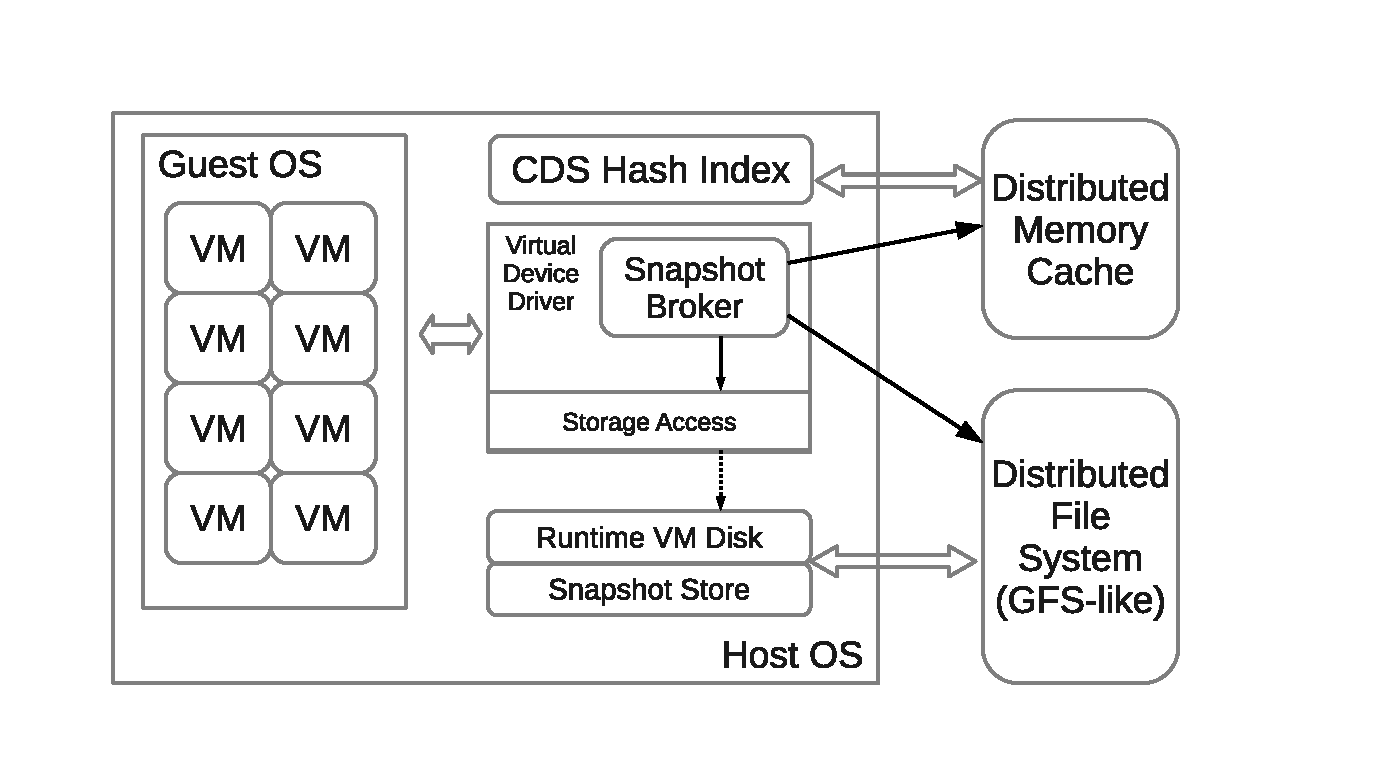
\epsfig{file=images/arch.eps, height=2in, width=2.66in}
%   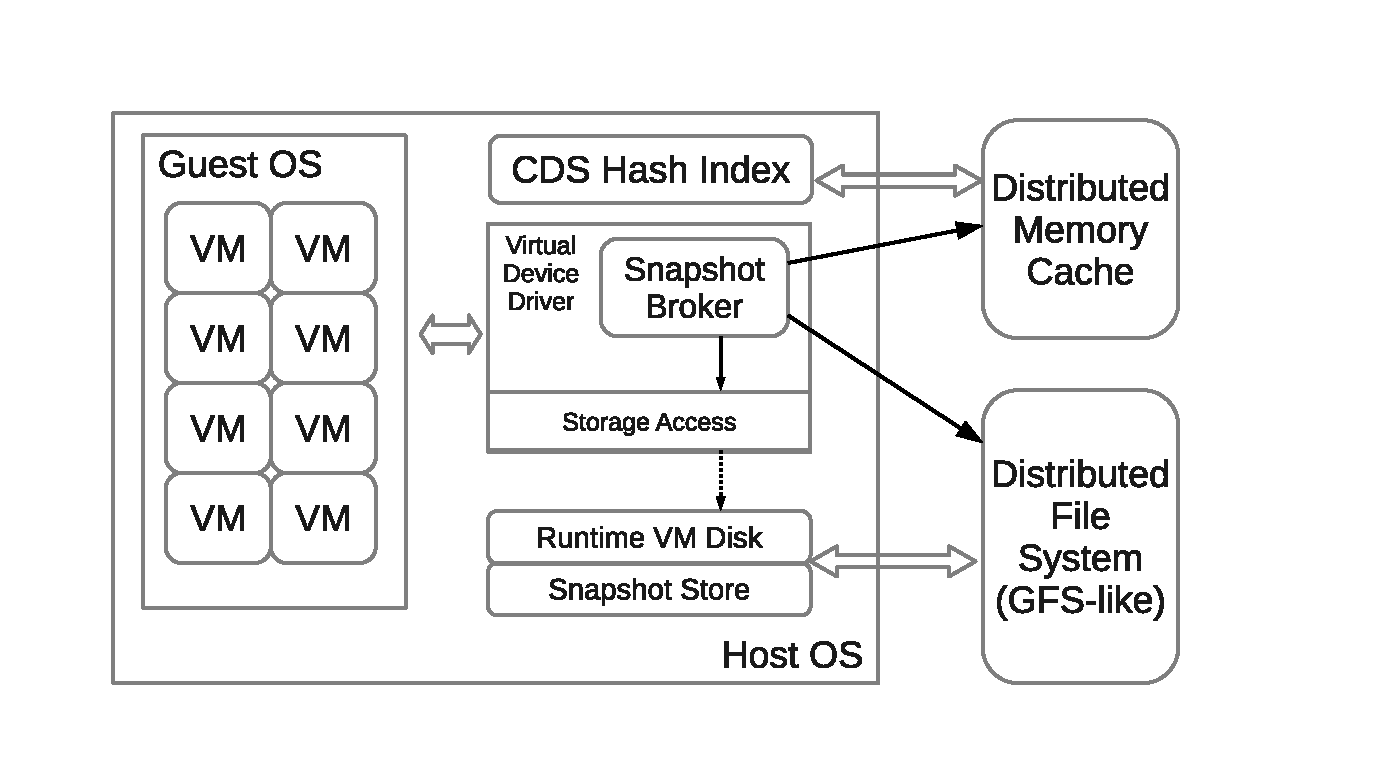
\epsfig{file=images/arch.eps, width=3.9in}
%   \caption{Snapshot backup architecture of each node.}
%   \label{fig:arch}
% \end{figure}
% The snapshot store 
% supports data access operations such as \emph{get}, \emph{put} and \emph{delete}.
% Other operations include data block traverse and resource usage report.
% The snapshot data does not need to be
% co-located with VM instances, and in fact they can even live in a different cluster to improve the 
% data reliability: when one cluster is not available, we are still able to restore its VMs from another cluster which
% holds its snapshot data. 
% %to reduce the impact to our users.
% %Get interface accepts a piece of data, write it to the underline data file, and return
% %a reference to the caller. This reference then can be used in the put interface to
% %retrive or delete the data, thus the caller of put interface must preserve the
% %data reference for future use. 
% %In addition to above standand data access operations, the snapshot service also supports
% %\emph{scan} and \emph{quota} methods. Scan allows us to traverse all the data blocks of each VM
% %in the snapshot store, and quota is used to acknowledge user how much space he
% %has actually used.

% Under the hood of snapshot store, it organizes and operates snapshot data 
% in the distributed file system. We let each virtual disk has its own snapshot store, 
% and no data is shared between
% any two snapshot stores, thus achieve great fault isolation. For those selected popular data
% that shared by many VM snapshot stores, we could easily increase its availability by having more replications.
% %Since all the underline data structures is append only,
% %upon a delete request, the corresponding data will only be marked rather than being deleted.
% %A compaction will take place when deleted data has accumulated to a certain threshold, thus 
% %reclaiming the disk space .


% \subsection{Block Storage Device}
\subsection{PDS}
Although locality based data reduction can remove most of the inner-VM duplications,
it's not able to solve the data duplication cross VMs. Different VMs still share large amount
of common data such that their snapshot backups would have a lot of data in common.
Our observations on Aliyun's real VM user data reveals several major sources of cross-VM data duplication:
  \begin{enumerate}
  \item \emph{System-related data}: These data are generated by public third-parties, they are copied/downloaded/installed into VM disks either automatically or manually. Once installed, operations on such data are mostly read only until software updates arrive. For example, data of operating systems, some widely-used software such as Apache and MySQL, and their documations all fall into this category.
  \item \emph{User-generated data}: These data are generated by individual user's behavior, either directly or indirectly. They are much less duplicated than the system-related data, but the zipf-like distribution indicates that a small amount of data in this category could represent most of data duplications.
  \item \emph{Zero-filled data}: Like previous studies [refs here], we've observed that zero-filled data exist pervasively at system wide. They are almost like the spaces and commas in text articles. Under content-based chunking, they were distilled as zero-filled blocks with the maximum allowed length. 
%Zero-filled blocks are mostly generated by user behavior to preserve the space for future data, thus we treat them as a special case of user-generated data.
  \end{enumerate}

Without eliminating the data duplication between VM snapshot backups, storage space is severely wasted when the number of VMs increases.
To address this problem, we developed a technique called \emph{Common Data Set (PDS)} to eliminate data duplication for all three situations above. 
PDS is a public data library that shared by all VM snapshot backups in the cluster, 
which consists of the most popular data blocks in VM snapshot backups. It is generated, 
managed and accessed in an uniform manner by all VMs such that [write some fancy system characteristic stuff here].

\subsection{PDS Size V.S. Coverage}
As a shared data library, we expect PDS to collect almost all the system related data, the most popular user-generated data and the zero-filled data block.
With PDS as a public data reference, each VM's snapshot backup has no need to store its own copies for data that can be found in PDS, instead they can just
store a reference.

The more data we put into PDS, the closer we come to complete deduplication. But in reality we are facing a list of restrictions such like [blabla].
We borrowed the idea of web caching[refs here] to analysis the size of PDS vesus its effectiveness on data reduction.

We let $M$ be the number of nodes in a cluster, $N$ be the number of VMs hosted per node,
and let $D$ denotes the average size of one VM's snapshot backups (after level 1 and 2 reduction, which is near 40 GB in our production environment).
And let $C_0$, $C_s$ and $C_u$ denote the size of zero-filled block, system-related data and user-generated data in PDS,
then the total size of PDS is represented by $C=C_0+C_s+C_u$.
We let $S_0$, $S_s$ and $S_u$ denote the corresponding data coverage ratio (with respect to $D$) by $C_0$, $C_s$ and $C_u$,
so the total space saving ratio is $S=S_0+S_s+S_u$.

Zero-filled block at maximum length is the first item we need to put into PDS. This is the one and only special data block, 
and because PDS only stores unique data blocks, $C_0$ is almost equal to 0. In practice we found zero-filled blocks account
for near 20\% of total data, so $S_0$ is 20\%.

The rarely modified system-related data are the second to be added to PDS. We have thousands of VMs in each cluster, 
but all these VMs fall into only a few OS types, using a limited selection of software, therefore data duplication in this category
is highly noticable in a global block counting. In particular, most of such data already exist in the VM base images. 
We analyzed VMs running various services from 7 mainstream OS types in our cluster, and found close to 50GB of such data in total. 
Because system-related data don't change frequently, it's safe to expect that for 20 OS variations 
and software updates in 2 years, $C_s$ will not grow to exceed 200 GB.
For each VM, from 2 to 20 GB of data can be reduced in this way, depends on the OS and service type, so on average we estimate
$S_s$ would be no less than 20\%.

The rest of data are user-generated, the total size of such data can be written as $D_u=D-S_0-S_s$, which is 60\% of $D$. 
It follows a zipf-like distribution with $\alpha$ between 0.65 to 0.7. 
Let $T_u$ be the total size of unique data blocks in $D_u$,
in practice we notice that complete deduplication for such data always result in a 2:1 reduction ratio,
, so $T_u=D_u/2$.
Since we collect the most popular user-generated data into PDS, the coverage of PDS on user-generated data
is $(C_u/T_u)^{1-\alpha}$.

The following table lists PDS coverage on user-generated data under different $\alpha$ and $C_u/T_u$.

[a table of coverage with alpha from 0.65-0.70, ratio from 0.002 0.005 0.01 0.02 0.05]

It's obviously that at least 30\% of user-generated data can be reduced in this way, using about 0.02 of $T_u$, or 0.01 of $D_u$.
The size of user-generated data in PDS would be 0.006$D$, with coverage $S_u=0.18D$.

Thus the estimation of PDS coverage is $S=S_0+S_s+S_u=0.58$, with the size of PDS to be no more than $(200 + 0.006*D*N)$ GB.
In a VM cluster of 100 machines, with 25 VMs on each physical machine, the size of PDS is 800 GB in total, or 8 GB per machine.
The total size of PDS index would be 8 GB, which will cost 80 MB memory on each machine. 

\subsection{Append Store}


\section{Background and Related Work}
\label{sect:background}


At a cloud cluster node providing access to multiple virtual machines, each
instance of a guest operating system runs on a virtual machine (VM), accessing
virtual hard disks represented as virtual disk image files in the host
operating system. For VM snapshot backups, file-level semantics are normally
not provided, and snapshot operations take place at the virtual device driver
level.  This meands no fine-grained file system metadata can be used to
determine the changed data.

Another issue is the sheer size of the backups. to maintain mutiple daily
uncompressed snapshots of each VM would be very expensive, even though
most of the data remains the same from day to day, and even between VMs common
software packages and operating systems mean that the amount of unique data is
much smaller. Backup systems have been developed to use content fingerprints to
identify duplicate content~\cite{venti02,Rhea2008}. Offline deduplication is
used in~\cite{EMC,NetAppOffline} to remove previously written duplicate blocks
during idle time.  Several techniques have been proposed to speedup searching
of duplicate fingerprints. For example, the data domain method
~\cite{bottleneck08} uses  an in-memory Bloom filter and a prefetching cache
for data blocks  which may be accessed.  An improvement to this work with
parallelization is in ~\cite{MAD210,DEBAR}.  As discussed in
Section~\ref{sect:intro}, there is no dedicated resource for deduplication in
our targeted setting and low memory usage is required so that the resource
impact to other cloud services is minimized. Approximation techniques which
reduce the memory requirement at the expense of deduplication efficiency are
studied in~\cite{extreme_binning09,Guo2011,WeiZhangIEEE}.  In comparison, this
paper focuses on full deduplication without approximation

%%In a virtualized cloud environment such as ones provided by Amazon EC2\cite{AmazonEC2} and Alibaba Aliyun\cite{Aliyun}, 
%At a cloud cluster node, each instance of a guest operating system runs on a virtual machine, accessing virtual hard disks 
%represented as virtual disk image files in the host operating system.
%For VM snapshot backup, file-level semantics are normally not provided.
%Snapshot operations take place at the virtual device driver level, which means no fine-grained file system metadata can be used to determine the changed data. 
%%Only raw access information at disk block level are provided. 
%%Each physical machine hosts many VMs and petabytes of data in a cloud cluster need a frequent  backup. 
%%Ideally speaking, snapshot backup must not affect the normal cloud service, which means that 
%%only a very small slice of cluster resource can be used for the backup purpose.



%%The previous work for storage backup has extensively used  data deduplication techniques can eliminate redundancy globally among different files from different users.
%Backup systems have been developed to use content fingerprints to identify duplicate
%content~\cite{venti02,Rhea2008}.
%Offline deduplication is 
%used in ~\cite{EMC,NetAppOffline} to remove previously written duplicate blocks during idle time.
%%,NGmiddleware2011}.
%%Today's commercial data backup systems (e.g. from EMC and NetApp)
%%\cite{emc_avamar}\cite{datadomain_whitepaper}
%%use a variable-size chunking algorithm to detect duplicates in file data~\cite{similar94,hydrastor09}.
%Several techniques have been proposed to speedup searching of duplicate
%fingerprints. For example, the data domain method ~\cite{bottleneck08} 
%uses  an in-memory Bloom filter and a prefetching cache for data blocks  which may be
%accessed.  An improvement to this work with parallelization is in ~\cite{MAD210,DEBAR}.
%As discussed in Section~\ref{sect:intro},
%there is no dedicated resource for deduplication in our targeted setting and low memory usage
% is required so that the resource impact to other cloud services is minimized.
%%NG et al.~\cite{ NGmiddleware2011}  use
%%a related filtering technique for integrating deduplication in Linux  file system and the memory
%%consumed is up to 2GB for a single machine. That is still too big in our context discussed below.
%%Lillibridge et al.~\cite{sparseindex09} break list of chunks
%%into large segments, the chunk IDs in each incoming segment are sampled and the segment is
%%deduplicated by comparing with the chunk IDs of only a few carefully selected backed up segments.
%%These are segments that share many chunk IDs with the incoming segment with high probability.
%The approximation techniques are studied in~\cite{extreme_binning09,Guo2011,WeiZhangIEEE}  
%%Deepavali et al.~\cite{extreme_binning09} and Zhang et al.~\cite{WeiZhangIEEE}  
%to reduce memory requirement with a tradeoff of the reduced deduplication ratio.
%%use fingerprint-based file similarity  and group similar files into the same physical location (bins) to deduplicate against each other.
%%That leads  to a smaller amount of memory usage for storing meta data in fingerprint
%%lookup  
%In comparison, this paper focuses on  full deduplication without approximation.
%%We also take advantages of the fact that in a VM cloud environment,
%%the virtual device driver can easily keep track if  large data
%%segments have been modified using dirty bits and such information can avoid sending
%%unmodified data segments for deduplication, which significantly saves cost.



Additional inline deduplication techniques are studied in ~\cite{sparseindex09,Guo2011,idedup}. 
All of the above approaches have focused on
such inline duplicate detection in which  deduplication of an individual block  is on the critical write path.
In our work, this constraint is relaxed and 
there is a waiting time for many duplicate detection requests. This relaxation is acceptable because 
in our context, efficiently finishing the backup of VM images within a reasonable time window is more
important than optimizing individual VM block  backup requests, and by batch
processing the deduplication requests we can decrease resource usage.




\comments{
This paper considers a backup service uses the existing cluster computing resource. 
Another option is to attach  a separate backup system with deduplication
support the cluster, and  every machine can periodically transfer snapshots to
the attached backup system.
%One  weakness of this approach is communication bottleneck between a large number of machines
%in a cloud to this centralized  service.
The cost of allocating the above dedicated backup  resource can be expensive.
Since most of backup data is not used eventually, CPU and memory resource in such a backup service may 
not be fully utilized. This paper seeks for a low-cost architecture option.
}
%It should be emphasized that our approach does not  accumulate raw backup data temporarily for deduplication
%and does not require a significant amount of extra storage capacity.
%Our strategy is to perform a drity  scan to collect
% a small amount of disk space  to accumulate
%deduplicate requests along with necessary meta data, and perform actual backup after deduplicate detection completes.
  
%affecting the overall time of backup. 

%\section{Design Consideration and Options}
%\label{sect:options}


\section{Background and Design Considerations}
\label{sect:option}


%In a virtualized cloud environment such as ones provided by Amazon EC2\cite{AmazonEC2} and Alibaba Aliyun\cite{Aliyun}, 
At a cloud cluster node, each instance of a guest operating system runs on a virtual machine, accessing virtual hard disks 
represented as virtual disk image files in the host operating system.
For VM snapshot backup, file-level semantics are normally not provided.
Snapshot operations take place at the virtual device driver level, which
means no fine-grained file system metadata can be used to determine the changed data. 
Backup systems have been developed to use content fingerprints to identify duplicate
content~\cite{venti02,Rhea2008}.  
As discussed earlier, collocating a backup service on the existing
cloud cluster avoids the extra cost to acquire a dedicated backup facility
and reduces the network bandwidth consumption in transferring the un-deduplicated
raw data for backup. 
Figure~\ref{fig:collocated} illustrates the cluster architecture where
each physical runs a backup service and a distributed file system (DFS)~\cite{GFS2004,Hadoop} 
serves a backup store  for the snapshots.
%The previous study shows that 
% deduplication can compress the backup copies 
%effectively in a 10:1 or even 15:1 rage. 
%Therefore  the portion of space in a cluster
%allocated for snapshots of data should not dominate
%the cluster storage usage.
%perhaps briefly discuss compression is high, incremental change is small from versions..???


%The running of such a service is subject to the resource availability of the system and 

% That arises mainly in Alibaba's Aliyun cloud service.
%concerns
%Base on Aliyun's production environment, the snapshot backup job has to satisfy 


\begin{figure}[htb]
    \centering
    \includegraphics[width=3in]{images/colocated-arch}
    \caption{Collocated VM Backup System.}
    \label{fig:collocated}
\end{figure}

%Only raw access information at disk block level are provided. 
%Each physical machine hosts many VMs and petabytes of data in a cloud cluster need a frequent  backup. 
%Ideally speaking, snapshot backup must not affect the normal cloud service, which means that 
%only a very small slice of cluster resource can be used for the backup purpose.



%The previous work for storage backup has extensively studied  data deduplication techniques that
%can eliminate redundancy globally among different files from different users.
%Offline deduplication is 
%used in ~\cite{EMC,NetAppOffline} to remove previously written duplicates during idle time.
%,NGmiddleware2011}.
%Today's commercial data backup systems (e.g. from EMC and NetApp)
%\cite{emc_avamar}\cite{datadomain_whitepaper}
%use a variable-size chunking algorithm to detect duplicates in file data~\cite{similar94,hydrastor09}.
Since it is expensive to compares a large number of chunk signatures for deduplication,
several techniques have been proposed to speedup searching of duplicate
fingerprints. For example, the data domain method ~\cite{bottleneck08} 
uses  an in-memory Bloom filter and a prefetching cache for data chunks  which may be
accessed.  An improvement to this work with parallelization is in ~\cite{MAD210,DEBAR}.
%As discussed in Section~\ref{sect:intro},
%there is no dedicated resource for deduplication in our targeted setting and low memory usage
% is required so that the resource impact to other cloud services is minimized.
%NG et al.~\cite{ NGmiddleware2011}  use
%a related filtering technique for integrating deduplication in Linux  file system and the memory
%consumed is up to 2GB for a single machine. That is still too big in our context discussed below.
%Lillibridge et al.~\cite{sparseindex09} break list of chunks
%into large segments, the chunk IDs in each incoming segment are sampled and the segment is
%deduplicated by comparing with the chunk IDs of only a few carefully selected backed up segments.
%These are segments that share many chunk IDs with the incoming segment with high probability.
The approximation techniques are studied in~\cite{extreme_binning09,Guo2011,WeiZhangIEEE}  
%Deepavali et al.~\cite{extreme_binning09} and Zhang et al.~\cite{WeiZhangIEEE}  
to reduce memory requirements with the tradeoff of a reduced deduplication ratio.
%use fingerprint-based file similarity  and group similar files into the same physical location (bins) to deduplicate against each other.
%That leads  to a smaller amount of memory usage for storing meta data in fingerprint
%lookup  
%In comparison, this paper focuses on  full deduplication without approximation.
%We also take advantages of the fact that in a VM cloud environment,
%the virtual device driver can easily keep track if  large data
%segments have been modified using dirty bits and such information can avoid sending
%unmodified data segments for deduplication, which significantly saves cost.
Additional inline deduplication techniques are studied in ~\cite{sparseindex09,Guo2011,idedup}. 
All of the above approaches have focused on optimization of deduplication
efficiency, and none of them have considered the impact
of deduplication on fault tolerance in the cluster-based environment that we have considered
in this paper.
%We will describe the motivation of using the cluster-based   approach
%for running the backup service and then present our solution  with fault isolation.
%In our work, the foucs 
%there is a waiting time for many duplicate detection requests. This relaxation is acceptable because 
%in our context, finishing the backup of required VM images within a reasonable time window is more
%important than optimizing individual VM block  backup requests.




%{\em Collocating with cluster-based cloud services.}
%We collocate the backup service with other cloud services in a cluster
%and use a distributed file system
%store the backup with multiple replicas. 
%There might be a concern that storing many versions of snapshots would
%go against the purpose of deduplication.

%Assume on the average the compression
%ratio is $c$:1.  When the number of versions
%saved in the backup storage is $l$  on the average, 
%the amount of storage space in the cluster allocated  for the backup would be $\frac{l}{l+c}$.
%For example, when $l=5$ and $c=10$, 33\% of the cluster storage is used for the backup.
%When $l=9$ and $c=13$, storage usage is 40\%. 
%That is acceptable given today's cheap cost for disk storage.
%In the case of Alibaba, each machine hosts 25 VMs on the average and each VM uses 40GB data.
%Each machine however can typically provide over 10TB storage.
%Thus the normal disk usage  is about 1TB per machine, and adding 30\% to 100\% 
%extra space for the backup is not a practical concern, especially with the
%added benefits of cheaper running costs and lower network bandwidth requirements.

Our key design consideration is VM dependence minimization during deduplication and file block management.
\begin{itemize}
\item {\em Deduplication localization.}
%Previous work in deduplication~\cite{extreme_binning09,sparseindex09} has
%studied the solutions to reduce memory requirements.
%One important issue not considered in the previous work is how 
Because a data chunk is compared with signatures collected from all VMs during
the deduplication process, only one copy of duplicates is stored in the storage,
this artificially creates data dependency among different VM users. 
Content sharing via deduplication affects fault isolation since machine failures happen periodically 
in a large-scale cloud and
%failure of a shared block affects many VMs.
%the loss of a shared chunks can affect many VM users whose snapshots share this 
%data block. 
loss of a small number of shared data chunks can 
cause the unavailability of snapshots for a large number of virtual machines.
Localizing the impact of deduplication can increase fault isolation and resilience.
Thus from the fault tolerance point of view,  duplicate sharing among multiple VMs is 
discouraged. 
Another disadvantage of sharing is that it complicates snapshot deletion, 
which  occurs frequently when snapshots expire regularly. 
The mark-sweep approach~\cite{mark-sweep} is effective for deletion, and its main cost
is to count if a data chunk is still shared by other snapshots.
Localizing deduplication can  minimize data sharing and simplify deletion while sacrificing 
deduplication efficiency, and  can faciltate parallel execition of snaptshot operations.
%Thus we seek for a tradeoff. 
 
% since storage for shared identical content chunks can become a failure point.
%Without any control of such data sharing, we can only increase  
%replication for global datasets to enhance the availability,
%but this incurs significantly higher costs.
%Thus a key goal  in our design
%is restricting the impact of  data loss to a limited number of VMs. 
%It is not desirable that small scale of data failure affects the backup of many VMs.
%when users access snapshots in a recovery process. 
\item{\em  Management of file system blocks.}
The file block size in a distributed file system such as  Hadoop and GFS is uniform and large (e.g.  64MB),
 a data chunk in a typical deduplication system is of a nonuniform size with 4KB or 8KB on average.
%We need to build an intermediate layer that supports large snapshot writing with append operations
%and infrequent snapshot access.
Packaging data chunks to a file system block can create more data dependence among VMs
since a file block can be shared with even more VMs.
Thus we need to consider a minimum association of a fie system block to VMs in the packaging process.
%The distributed file system~\cite{GoogleFS,Hadoop} provides the replication support
%and we can leverage existing open-source software to implement such a layer.
%When the number of machines failed exceeds the replication degree, there could be
% some data loss.  
%Storage deduplication worsens the impact of such faults
%because  the majority of each snapshot (e.g. over 90\%) is deduplicated
%and the corresponding data chunks stored in the underlying file blocks
%are shared by many VMs. 
%The failure of one data chunk or block can impact many sharing VMs. 
\end{itemize}

%\item {\em Requirement for backup throughput and low computing resource usage}.
Another consideration is the computing cost of deduplication.
Because of collocation of this snapshot service with other existing cloud services, 
%As a large-scale cluster hosting tens of thousand of active VMs everyday,  the amount of data
%to be processed can be huge. 
cloud providers wish that the backup service only consumes  small resources
with a minimal impact to the existing cloud services.
%the computing resources allocated for the snapshot service is limited, especially
%because of its lower priority.
The key resource for signature comparison  is memory for storing the fingerprints. 
We will consider the approximation techniques with less memory consumption along 
with the fault isolation consideration discussed below. 
%A snapshot backup service shall not compete cpu, memory, or I/O bandwidth with VMs. 
%Fingerprint-based search does require a significant amount of memory for fingerprint lookup
%and comparison.  This competes memory resource  with the existing VMs.
%Our design is to identify a low-cost and low-profile scheme for deduplication.
%Specifically, the memory usage of snapshot service can never exceed 500MB in any node.
%Excessive use of bandwidth and computing resource for backup can create
%noticeable contention for resources with the existing cloud, which is not
%preferred and may not not be acceptable for production system operation. 
%Thus it is desirable that backup for all nodes
%can be conducted in parallel and in a short period of time,
%and any centralized or cross-machine communication for
%deduplication should not become a bottleneck.
%For example, in an Aliyun cluster with over 1,000 nodes and each hosts over 25 VMs, 
%the system must finish saving daily snapshots of all VMs in a few hours. 
%Often a cloud has a few hours of light workload each day (e.g. midnight),  
%which creates an small window for automatic backup.
%The backup service can generate hundreds of terabytes of data in such a time window
%without optimization and thus the resource content is considered carefully as we design
%a fault-resilient cluster-based solution. 
%In our typical 1000 nodes cluster, each node hosts 25 VMs, each VM has 40GB of data on average, that translates to backup throughput of 139GB/second, or 
%500TB/hour.  The system must finish saving daily snapshots of all VMs in few hours. 

%At Aliyun, it is required that while CPU and disk usage should be small or modest during backup time,
%the memory footprint of snapshot service should not exceed 500MB at each node.


\comments{
Another consideration is backup data cleaning to delete useless blocks.
Keeping reference counters for shared data blocks is challenging and less reliable.
The previous work has advocated the mark-and-sweep approach  which periodically
scans all data (or modified latest version of data)~\cite{?, Guo2011}. It first marks
all used blocks and then sweep all chunks to reclaim unmarked blocks. 
This approach is resilient to errors: at any time the process can simply be restarted with no 
negative side effects.  Scalability, however, is an issue.
To deal with 1 PB snapshots data, which may be represented by 10,000 GB FP index,
If we account for an average deduplication factor of 10 (i.e., each chunk
is referenced by 10 different snapshots), the total size
of snapshot metadata that need to be read during the mark phase will
be 100 TB.  This alone will take almost 2 hours on a
1000-machine cloud. Furthermore, marking the in-use
bits for 250 billion entries is no easy task. There is no
way to put the bit map in memory. One might want
to mitigate the poor performance of mark-and-sweep by
doing it less frequently. But in practice this is not a viable
option: customers always want to keep the utilization
of the system close to its capacity so that a longer
history can be stored. With daily snapshots taking place,
systems rarely have the luxury to postpone deletion operations
for a long time. In our field deployment, deletion
is done once a day. More than 2 hours in each run is too
much. In a large production-oriented deduplication system reference
management needs to be very reliable and have
good recover-ability. It should tolerate errors and always
ensure correctness. Although mark-and-sweep provides
these properties, its performance is proportional to the
capacity of the system, thus limiting its scalability.

}



%we want to isolate 
%each VM's snapshot backup as much as possible while still enjoy the benefit of deduplication.
%In large scale cloud, node faiures happen at daily basis, we don't want a problem at small scale
%to affect large amount of VMs due to data sharing.
%a key weakness of global content fingerprint comparison is that it affects fault isolation.

%2) data sharing among users for accessing common signagutes causes the system less resilient to storage failures.
%any loss of one piece of  shared data content hash and actualcontent will damange many VM snapshots, which can cause massive impacts
%on reliability of many users.

%Another point is that the previous work in signature-based comparison does not address
%load balancing for a distributed environment during parallel access.  
%Some content signatures can be extremely hot, but the machines  that  handle such signatures can become
% a bottleneck. Uncoordinated signature assignment could lead to imbalanced access workload.


%There are multiple choices of snapshot backup design for VM images and our considerations are described
%as follows. 
%Our design considerations
%\begin{enumerate}
%\item {\bf Centralized vs. decenalized} 
%
%It is desirable to have  a decentralized architecture.
%Given a large amount of snapshot data communicated from each machine to the backup storage,
%with a distributed storage architecture for backup, one could exploit  exploit data locality between
%the source of data and storage location of data to reduce cross-platform bandwidth requirement for backup.

%execute in parallel and easy to coordinate. In fact, we want to avoid cross-node dependency at scheduling VM snapshot operations, such that no global coordinator is necessary.
%\item {Load balancing in resource consumption}: the cost of snapshot service shall be evenly distributed onto every node. We don't have a super powerful
%or stable node that can accept extra responsibility.
%\item {minimization of inter-user data dependency for fault tolerance}: we want to minimize the data dependency to a controllable level. Data deduplication means sharing of data, thus one failure at a single point may affect the snapshot service of hundreds of VMs, which is absolutely unacceptable.
%\item {Resource usage modeling and control}.
%\end{enumerate}


We call the traditional deduplication approach as   VM-oblivious (VO)
because they compare fingerprints of snapshots without consideration of VM.
With the above  considerations in mind, we study a 
VM-centric approach (called VC)
for a collocated backup service with resource usage friendly
to the existing applications.  
%We will first discuss and analyze the integration of the VM-centric deduplication strategies with fault isolation, and then present
%an architecture and implementation design with deletion support.
%The traditional approach compares all fingerprints and
%stores one copy for all of a chunk's duplicates.
In designing a VC duplication algorithm, we have considered and adopted some of
the following previously-developed techniques.
\begin{itemize}
\item {\bf Version-based change detection}.
VM snapshots can be  backed up  incrementally by identifying file  blocks that have
changed from the previous version of the snapshot~\cite{Clements2009,Vrable2009,TanIPDPS2011}.
Such a scheme  is  VM-centric since deduplication is localized. 
%Active snapshots will contain all the information needed to restore the virtual disk
%and when deleting a snapshot, data referenced by other snapshots are removed.
We are seeking for a tradeoff since 
cross-VM  signature comparison can deliver additional compression~\cite{Guo2011,Dong,ExtremeBining}.
%We are seeking for additional optimization to improve duplication efficiency and design the 
%association of data chunks with the underlying file blocks so that
%file block sharing among VMs is minimized.
\item {\bf Stateless  Data Routing}.
One approach for scalable duplicate comparison is to use a content-based hash
partitioning algorithm called stateless data routing~\cite{Dong20??}
that divides the deduplication work with an approximation. This work 
is similar to Exreme Binning\cite{extreme_binning09} and 
each request is routed  to a machine which holds
a bloomer filter  or can fetch on-disk index for additional comparison.
While this approach is VM-oblivious, it motivates us to  use  a combined signature of a dataset to narrow
VM-specific local search.
 
%We compared our solution to
%content-based hash partitioning by running the algorithm on our set of 
%traces. We used 2MB superchunks and 4KB chunks to partition the data, and use
%the minhashes of the superchunks for routing. The results of this are shown in
%Table~\ref{??}. Routing each chunk to a bin provides good deduplication
%efficiency, and only requires each storage node to keep an index of local data
%and the bin mapping, but misses significant opportunities in our indended use
%case.

%The problem with the Data Routing algorithm is in the very high network traffic.
%Our intended use case is a backup system which runs alongside a number of VMs,
%in order to save costs. Data Routing makes no use of the inherent locality in
%such a system, and therefore puts a much higher network burden on machines which
%are also running 35 VMs each. This will reduce the available network bandwidth
%to users of the VMs, and/or reduce the possible deduplication throughput.
\item {\bf Sampled Index}.
One effective approach that reduces memory usage is 
to use a sampled index with prefetching, proposed  by Guo and Efstathopoulos\cite{Guo2011}. 
%An evaluation with our test data shows that using a sampled index can achieve a high
%deduplication efficiency with a single machine setup.  
The algorithm is VM oblivious and it is not easy  to adopt for a distributed architecture. 
%The algorithm stores the sampled index in memory, which is required for high
%throughput to avoid the disk-bottleneck problem - since the index itself has no
%locality information, lookups are essentially random, so the index must be
%somehow optimized to prevent excessive disk seeking (the sampling algorithm does
%this by storing the index in memory). 
To use a distributed memory version of the sampled index, every deduplicate request
may access a remote machine for index lookup and the overall overhead of latency latency for all requests
can be significant.  


%Another possibility is to use this approach partially  in our VM centric solution by indexing
%the most popular data chunks. For a small set of popular data chunks, the prefetching strategy
%used in the sampled index will not work well because the spatial locality is limited among popular 
%data chunks. In our test data,  on average the number of consecutive data chunks is 7, which is too small
%to be effective for index sampling. 

%To distribute this sampled index, every  each machine would
%either require a complete copy of the index which would have a prohibitive cost in
%memory, or something like memcached must be used, which leaves the same problem
%as the disk bottleneck with every index check potentially using the network.
%The difficulty in storing extremely large bodies of data
%is related, as once 1PB is stored in the system, assuming a sampling rate of 
%1/101 with 22 byte index entires, 55GB of (in memory) index are required.

%Our solution uses more total memory (??how much??), but is more scalable both in
%terms of capactity and distributing the deduplication. The only part of our
%algorithm which requires significant network traffic is the PDS deduplication,
%but this is done after Levels 1 and 2 (dirty bits and comparison to parent), and
%so is only done for a small percent of blocks (?? 5-10\% ??).
\end{itemize}

%With these considerations in mind, we study a 
%VM-centric approach (called VC)
%for a backup service co-hosted   in the existing set of machines and resource usage is friendly
%to the existing applications.  
We will first discuss and analyze the integration of the VM-centric deduplication strategies with fault isolation, 
and then present
an architecture and implementation design with deletion support.

%The deduplication process is first conducted among snapshots within each VM
%and then is conducted across VMs.  
%Given the concern that searching duplicates across VMs is a global feature which can affect parallel performance
%and complicate failure management,
%we only eliminate the duplication of a small but popular data set while still maintaining a cost-effective deduplication ratio.
%For this purpose, we exploit the data characteristics of snapshots and collect most popular data.
%Data sharing across VMs is limited within this small data set such that adding replicas for it could enhance fault tolerance.
%
%in the  our studies show that there are a large amount of data unmodified in VM snapshots
%and shared among many users (e.g. OS data). The sharing pattern follows a zip-like distribution.
%With this characteristic, we can store a small amount of popular data items which coverage a large amount of
%snapshot data blocks. 
%We discuss our design and data analysis in the next section.


%This method is based on the observation of two facts in Aliyun's VM cloud: first, VM's OS disks contain 
%huge amount of operating system and software related data which is almost never modified during VM's life span. 
%Second, the duplication pattern of user generated data follows Zipf-like law, thus a tiny set of hottest data
%take up the majority of data duplication. As a result, if we extract these hot data as a common data set,
%then most of data duplication will emerge by searching in this very small scope.


%For example, In cloud storage, we are solving data deduplication problem in a different context of 
%data stream deduplication (the D2D case): our snapshot storage service is co-located with runtime VMs,
%thus we have very limited amount of system resource leave for data deduplication. For example,
%in Aliyun's 8-core, 48GB memory, 12TB VM server, there lives over 20 VMs who are hungrily competing for
%system resources: some may running map-reduce jobs, some may serving busy web requests, 
%some may storing backend databases, any behavior that affects user VMs performance or stability is unacceptable.

%To reduce the cost of deduplication, we must confine the scope of searching duplicates as much as possible,
%thus some hints are needed to tell us where the most likely duplicates would hide. 
%Several form of hints have been used in the past: many D2D systems exploits locality,
%which bases on the fact that duplicates are likely to appear in the same sequence as they have arrived before.
%Similarity is another popular hint, it suggests that two sets of data blocks may contain lots of
%duplicates if they are indetified as similar by certain similarity detection measurements.



%\section{Architecture design and Deduplication for Snapshot Support}
%
%\section{Popularity analysis}
% data on what data popular.
%
%Analysis: modeling: singular
%
%Compute: Cache hit ratio vs. cache cost (memory cost).


\comments{
\section{Challenges}
\subsection{Indexing}
Most deduplication systems operate at the sub-file level:
a file or a data stream is divided into a sequence of fixed
or variable sized segments. For each segment, a cryptographic
hash (MD5, SHA-1/2, etc.) is calculated as its
fingerprint (FP), and it is used to uniquely identify that
particular segment. A fingerprint index is used as a catalog
of fingerprints stored in the system, allowing the detection
of duplicates: during backup, if a tuple of the form <
FP, location > exists in the index for a particular
FP, then a reference to the existing copy of the chunk
is created. Otherwise, the chunk is considered new, a
copy is stored on the server and the index is updated accordingly.
In many systems, the FP index is also crucial
for the restore process, as index entries are used to locate
the exact storage location of the chunks the backup
consists of.

The index needs to have three important properties:
1) scale to high capacities, 2) achieve good indexing
throughput, and 3) provide high duplicate detection
rate—i.e., high deduplication efficiency. Table 1 demonstrates
how these goals become very challenging for a
Petascale system. Consider a typical virtualized cloud 
in which 10,000 VMs store 1 PB data, and the
chunk size is 4 KB (for fine-granularity duplicate detection),
indexing capacity will need to be at least 10,000
GB to support all 250 billion objects in the system. Such
an index is impossible to maintain in memory. Storing it
on disk, however, would greatly reduce query throughput.
To support 1000 concurrent snapshot backup tasks, 
an aggregate throughput of 20 GB/sec, would require the
index and the whole deduplication system for that matter
to provide a query service throughput of at least 5,000
Kops/sec. Trying to scale to 1 PB by storing the index
on disk would make it impossible to achieve this level
of performance. Making the chunk size larger (e.g.,
128 KB) would make deduplication far more coarse and
severely reduce its efficiency.

Even we can distribute the index over the cloud machines,
the resources that can be allocated to system services are
limited to minimize the negative impact to user experiences. 
So it becomes obvious that efficient, scalable indexing is
a hard problem. On top of all other indexing challenges,
one must point out that chunk FPs are cryptographic
hashes, randomly distributed in the index. Adjacent index
entries share no locality and any kind of simple readahead
scheme could not amortize the cost of storing index
entries on disk.


\subsection{Deletion}
Contrary to a traditional backup system, a dedupe system
shares data among files by default. 
Since snapshots in VM cloud face constant deletion, 
reference management
is necessary to keep track of chunk usage and reclaim
freed space. In addition to scalability and speed, reliability
is another challenge for reference management.
If a chunk gets freed while it is still referenced by snapshots,
data loss occurs and files cannot be restored. On the other
hand, if a chunk is referenced when it is actually no
longer in use, it causes storage leakage.

For simplicity, many previous works only investigated simple reference
counting without considering reliability
and recoverability. Reference counting, however, suffers
from low reliability, since it is vulnerable to lost or repeated
updates: when errors occur some chunks may
be updated and some may not. Complicated transaction
rollback logic is required to make reference counts consistent.
Moreover, if a chunk becomes corrupted, it is
important to know which files are using it so as to recover
the lost segment by backing up the file again. Unfortunately,
reference counting cannot provide such information.
Finally, there is almost no way to verify if the
reference count is correct or not in a large dynamic system.
Our field feedback indicates that power outages and
data corruption are really not that rare. In real deployments,
where data integrity and recoverability directly
affect product reputation, simple reference counting is
unsatisfactory.

Maintaining a reference list is a better solution: it is
immune to repeated updates and it can identify the files
that use a particular segment. However, some kind of logging
is still necessary to ensure correctness in the case of
lost operations. More importantly, variable length reference
lists need to be stored on disk for each chunk.
Every time a reference list is updated, the whole list (and
possibly its adjacent reference lists—due to the lists’
variable length) must be rewritten. This greatly hurts the
speed of reference management.

Mark-and-sweep is generally a better solution. 
During the mark phase, all snapshot metadata are traversed 
so as to mark the used chunks. 
In the sweep phase all chunks are swept and unmarked chunks are reclaimed. 
This approach is very resilient to errors: 
at any time the process can simply be restarted with no negative side effects. 
Scalability, however, is an issue.
To deal with 1 PB snapshots data, which may be represented by 10,000 GB FP index,
If we account
for an average deduplication factor of 10 (i.e., each chunk
is referenced by 10 different snapshots),
the total size
of snapshot metadata that need to be read during the mark phase will
be 100 TB. 
This alone will take almost 2 hours on a
1000-machine cloud. Furthermore, marking the in-use
bits for 250 billion entries is no easy task. There is no
way to put the bit map in memory. One might want
to mitigate the poor performance of mark-and-sweep by
doing it less frequently. But in practice this is not a viable
option: customers always want to keep the utilization
of the system close to its capacity so that a longer
history can be stored. With daily snapshots taking place,
systems rarely have the luxury to postpone deletion operations
for a long time. In our field deployment, deletion
is done once a day. More than 2 hours in each run is too
much. In a large production-oriented dedupe system reference
management needs to be very reliable and have
good recoverability. It should tolerate errors and always
ensure correctness. Although mark-and-sweep provides
these properties, its performance is proportional to the
capacity of the system, thus limiting its scalability.

\subsection{Fault Tolerance}
Because deduplication storage system
 artificially creates data dependency among different VM users,
it increases the risk of data availability.
In large scale cloud, node failures happen at daily basis,
the loss of access to a shared chunk can affect many VMs whose snapshots share this chunk. 
Without any control of the scope of data sharing, we can only increase the level of 
replication to enhance availability, which would significantly 
balance out the benefits of deduplication.

}

\section{VM-centric Snapshot Deduplication}
\label{sect:dedupe}
%snapshot representation

%We use the The deduplication process is first conducted among snapshots within each VM
%and then is conducted across VMs.
%Given the concern that searching duplicates across VMs is a global feature which can affect parallel performance
%and complicate failure management,
%we only eliminate the duplication of a small but popular data set while still maintaining a cost-effective deduplication ratio.
%For this purpose, we exploit the data characteristics of snapshots and collect most popular data.
%Data sharing across VMs is limited within this small data set such that adding replicas for it could enhance fault tolerance

%A deduplication scheme compares the fingerprints of the current snapshot
%with its parent snapshot and also other snapshots in the entire cloud.
%The traditional approach compares all fingerprints and 
%stores one copy for all of a chunk's duplicates.
%We call this as  the VM-oblivious (VO) approach.
Our VC design has the following  objectives: 1)  localizing deduplication while identifying a decent amount of
duplicates among VMs to maintain a competitive deduplication efficiency and simplify snapshot management;
2) Minimizing the number of file system blocks shared among VMs and adding extra replicas for shared blocks.

\comments{
\begin{itemize}
\item
1) Localize the deduplication and data blocking within each VM as much as possible so 
that any failure of a file system block mainly affects the associated VM.
Localizing the snapshot data deduplication within a VM
improves the system by increasing data independence between different VM backups,
simplifying snapshot management and statistics collection,
and facilitating parallel execution of snapshot operations.
\item
2) Maintain a competitive deduplication efficiency while being resource-friendly to other
existing cloud services.
Cross-VM duplication can be desirable since  there are many cloud images
use widely-used software and libraries and their data blocks are duplicate. 
As the result, different VMs tend to backup large amount of highly similar data.
\item
\end{itemize}
}
\subsection{Key VM-centric  Strategies}
\label{sect:vc-strategies}

%Inner-VM duplication can be very effective within VM's snapshots. There
%are typically a large number of duplicates existing among the snapshots
%for a single VM.  

%Our multi-level pipeline process can minimize 
%the cost of deduplication while maximize the its efficiency at each level,
%and it is parallel since each segment is processed independently.

%Our VC differentiates duplicates within a VM and cross VMs,
%and conducts \textit{Inner-VM} and \textit{cross-VM} detection separately. 

\begin{itemize}
\item \textbf{VM-specific local duplicate search within similar segments.}
We start with the standard dirty bit approach in a coarse grain segment level.
In our implementation with Xen at an Alibaba platform, the segment size is 2MB
and  the device driver is extended to support  changed block tracking. 
Since every write for a segment will touch a dirty bit, the device driver maintains dirty bits in memory
and cannot afford a small segment  size.
%Xen doesn't directly support it, However, their open-source 
%architecture allows anyone to extend 
%and use the  Xen virtual device driver to implement a feature called ``changed block tracking''
%for the storage device and the dirty bit setting is maintained in a coarse grain level we call it a segment.
It should be noted that dirtybit tracking is supported or can be easily implemented in 
major virtualization solution vendors. For example,
%(VMware, Xen, Microsoft).  
%VMware support it directly; 
the VMWare hypervisor has an API to let external backup applications know 
the changed areas since last backup. 
%We implement dirty bit tracking this way in Alibaba's platform.  
The Microsoft SDK provides an API that allows external applications to monitor 
the VM's I/O traffic and implement  the changed block tracking feature.

Since the best deduplication uses a nonuniform chunk size 
in the average of 4K or 8K~\cite{??},  
%This allows the system to achieve deduplication even when there are insertions/deletions which would
%affect many fixed-size chunks.
we conduct additional local inner-VM deduplication by comparing
dirty segment's chunk fingerprints to similar segments from its parent snapshot. 
For every segment, the minimum value of all its chunk fingerprints is computed during backup
and is recorded in the snapshot recipe.
When we are processing a dirty segment,
we can easily find similar segments from the
parent snapshot recipe and load their segment recipes. Then 
given a set of data chunks within a dirty segement,  we compare  these chunk fingerprints
with those in similar segments.  
For example, with a 2MB segment, there are about 500 fingerprints to compare.
The amount of memory for maintaining those fingerprints in similar segment s is small, as we only
load one dirty segment at a time.


%If we use 4KB in level-1, then such a level-1 should have similar dedup efficiency 
%as the current level-1 and level-2 combined, because finally they equal to comparing  
%parent snapshot at 4KB granularity.
%
%However, at level-3 things are different. If we use 4KB fix-size block uniformly, it would be harder for different VM to share data through PDS, because there is no guarantee that the location of duplicate data on different VM disks are always aligned at 4KB boundary. For example, if two VMs each has a copy of duplicate data, but they are not aligned, then we won't be able to detect them. Our study at the current small data set has shown that using 4KB fix-size block will make PDS method less efficient by nearly 10%. Over the long time, more and more OS variations will co-exist in the cluster, making this 4KB fix-size approach inefficient in reducing duplicate data across VMs.

%\item \textit{Level 2  Chunk fingerprint comparison.}
%If a segment is modified, we perform fine-grained deduplication 
%by comparing the fingerprints of its chunks to the same segment's recipe in the previous snapshot,
%thus eliminate partial data duplication within the segment.
%\end{itemize}
%
%In general, operations at level 1 have almost no cost and most of unmodified data are filtered here. 
%To process a dirty segment at level 2, 
%there requires no more than one DFS access to load the segment recipe from previous snapshot,
%and a tiny amount of memory to hold it in main memory.

\item \textbf{Cross-VM deduplication with popular chunks and replication support}
This step accomplishes the standard global fingerprint  comparison as conducted
in the previous work~\cite{??}.
One key observation is that the inner deduplication has removed many of the duplicates.
There are fewer deduplication opportunities across VMs while the memory and network
consumption for global comparison is more expensive.
Thus our approximation is that the global fingerprint comparison only searches for the top $k$
most popular items. This dataset is called PDS (common data set). 
%Since duplicate sharing patterns among  VM follows a zip-like distribution,  
The popularity of a chunk is the number  of data chunks  from different VMs
that are duplicates of this chunk after the inner VM deduplication.
This number can be computed periodically on a weekly basis.
Once the popularity of all data chunks is collected, the system only maintains the top $k$
most popular chunk signatures in a distributed shared memory.  
%For cross-VM comparison, we only store  top $k$ items and $k$ is chosen to be relatively small.

Since $k$ is relatively small and these top $k$ chunks are shared among multiple VMs, 
we can afford to provide extra replicas for these popular chunks to enhance the fault resilience.
%We will provide an analysis of the space need and fault tolerance in the next subsection.

\item \textbf{VM-centric file system block management.}
When a chunk is not detected as a duplicate to any existing chunk, this chunk will be written
to the file system. Since the backend file system typically uses a large block size such as 64MB, each VM will 
accumulate small local chunks. We manage this accumulation process using an append-store  scheme
and discuss this in details in Section~\ref{sect:arch}.
The system allows all machines conduct the backup in parallel in different machines, and each machine
conducts the backup of one VM at a time, and thus only requires a write  buffer for one VM.

PDS chunks are stored in a separate append-store instance. In this way, each
file block for non-PDS chunks is associated with one VM and does not contain
any PDS chunks. 
\end{itemize}

We have not  adopted the  sampled index~\cite{Guo2011} 
for  popular data chunks and  this is because sampling requires the use of prefetching to be effective.
%For a small set of popular data chunks, the prefetching strategy
%used In the sampled index will not work well because 
For the data sets we have tested, the spatial locality is limited among popular
data chunks and  on average the number of consecutive data chunks is 7 among popular chinks, which is not sufficient.
%to be effective for index sampling.


 \subsection{Impact on deduplication efficiency}
%VM-oriented Fault Isolation}
%Our objective for fault isolation is to minimize the number of VMs affected when there are failures
%in the cluster.  
%The inner-VM deduplication does not depend on any global service and the comparison
%for each VM is localized within the parent and the current snapshot.
%Lack of data dependence between VMs brings 
%Our analysis below will show that the algorithm can still deliver competitive
%deduplication efficiency after making these approximations.
%With cross-VM deduplication, shared data chunks
%create an artificial dependence  among VMs. 
%Thus we only maintain the index for the most popular chunks to reduce the inter-VM dependence
%while still accomplishing competitive deduplication efficiency. 

%The management for popular data chunks contains two aspects.



We analyze how the choice of value  $k$ impacts the deduplication efficiency.
%It also  compares the  fault resilience of our VM-centric deduplication approach with a standand approach using 
%global deduplication.
%\subsubsection{Impact of PDS deduplication}
The analysis is based on the characteristics  of the VM snapshot traces
studied from  Alibaba's production user data.
Our previous study shows that the popularity of data chunks after inner VM deduplication follows 
a Zipf-like distribution\cite{zipf} and its
exponent $\alpha$ is ranged between 0.65  and  0.7.~\cite{ieeecloud}. 
%As a result, it can be proved that deduplication efficiency of PDS index is scalable:
Table~\ref{tab:symbol} lists parameters used in this analysis.


\begin{figure}
\centering
%\epsfig{file=log-log.disk,width=3in}
%source ../vm_snapshot_sim/images/log-log.disk.eps
 \includegraphics[width=3in]{figures/log-log-disk}
\caption{Duplicate frequency versus  chunk ranking in a log scale.}
\label{fig:Datazipf}
\end{figure}

\begin{table}[ht]
\centering
\begin{tabular}{|p{1.25cm}|p{6.5cm}|}
\hline
$k$ &  the number of top most popular chunks\\ 
\hline
$c$ &  the total amount of data chunks\\ 
\hline
$c_u$ &  the total amount of unique fingerprints after inner VM  deduplication\\
\hline
$f_i$ &  the frequency for the $i$th most popular fingerprint\\
\hline
$\delta$ &  the percentage of duplicates detected in inner VM deduplication\\
\hline
$\sigma$ &  the number of unique non-PDS chunks over  the number of the PDS chunks.\\
\hline
$p$ & the number of machines in the cluster\\
\hline
$V$ & the number of VMs on each machine\\
\hline
$D$ & the amount of unique data on each machine\\
\hline
$C$ & the average data chunk size. Our setting is  4K.\\
\hline
$s$ & the average size of file system blocks in the distributed file system. The default is  64MB.\\
\hline
$m$ & memory size on each node used by VC\\ 
\hline
$E$ & the size of an popular data index entry\\
\hline
$N_1$ & the average number  of non-PDS file system blocks  in a VM\\
\hline
$N_2$ & the average number  of PDS file system blocks  in a VM\\
\hline
$N_o$ & the average number  of file system blocks  in a VM for VO\\
\hline
\end{tabular}
\caption{Modeling  parameters and symbols.}
\label{tab:symbol}
\end{table}

{\it [Need to find a place to put these numbers in: Total number of chunks 
in 350 snapshots: 1,546,635,485. 
Total number of chunks after localized dedup: 283,121,924. Total number of unique chunks: 87,692,682.]}

As summarized in Table~\ref{tab:symbol},
let $c$ be the total number of data chunks. 
$c_u$ be the total number of fingerprints 
in the global index after complete deduplication, and
$f_i$ be the frequency for the $i$th most popular fingerprint. 
By Zipf-like distribution, $f_i = \frac{f_1}{i^\alpha}.$
Since $ \sum_{i=1}^{c_u}f_i = c$,
\[
f_1 \sum_{i=1}^{c_u}\frac{1}{i^\alpha} = c.
\]
Given $\alpha <1$, $f_1$ can be approximated with integration:
\begin{equation}
f_1=\frac{c(1-\alpha)}{c_u^{1-\alpha}}.
\end{equation}

%We define deduplication efficiency $e$ to be the proportion of raw data that can be deduplicated,
%In complete deduplication scenario, it deduplication efficiency $e_c$ is:
%\begin{equation}
%e_c = \frac{b-b_u}{b} = 1 - \frac{b_u}{b}
%\end{equation}

The  $k$ most popular fingerprints can cover the following number of chunks after inner VM 
deduplication:
\[
f_1 \sum_{i=1}^{k}\frac{1}{i^\alpha} \approx  
f_1 \int_{1}^{k}\frac{1}{x^\alpha} dx  \approx  f_1\frac{  k^{1-\alpha}} {1-\alpha}.
\]

Deduplication efficiency of VC using top $k$ popular chunks
is the percentage of duplicates that can be detected:  
\begin{equation}
%\begin{split}
%e_k &= 
\frac{ c(1-\delta) + f_1\frac{  k^{1-\alpha}} {1-\alpha}} 
{c(1-\delta)  + \delta c - c_u }\\
= 
\frac{ (1-\delta) + \delta  (\frac{k}{c_u})^{1-\alpha}}
{ 1- \frac{c_u}{c} }.
%\end{split}
\end{equation}


%\begin{equation}
%\begin{split}
%e_k &= (\sum_{i=1}^{k}C_i - k)/{b} = (b * \frac{1-\alpha}{b_u^{1-\alpha}} * \sum_{i=1}^{k}\frac{1}{i^\alpha} - k)/b \\
%&\approx \frac{b*\frac{1-\alpha}{b_u^{1-\alpha}}*\frac{k^{1-alpha}}{1-\alpha} - k}{b}
%&\approx (\frac{k}{b_u})^{1-\alpha} - \frac{k}{b} \approx (\frac{k}{b_u})^{1-\alpha},\; (since\; k \ll b)
%\end{split}
%\end{equation}

% For the Zipf-like distribution, an approximation to the sum of the first $n$ 
% elements of the distribution can be derived as follows:
% \begin{equation}
% \sum_{i=1}^{n}\frac{1}{i^\alpha}\approx \int_{1}^{n}\frac{1}{x^\alpha}\mathrm{d}x=\frac{x^{1-\alpha}}{1-\alpha}=\frac{n^{1-\alpha}}{1-\alpha}\;  for\;  \alpha<1
% \end{equation}

% So the cumulative distribution function for a PDS holding top $S_c$ fingerprints
% of global index with size $S_g$ is:

% \begin{equation}
%   E = (S_c / S_g)^{1-\alpha} \;  for\;  \alpha<1
% \end{equation}

%[Describe the dedup efficiency model in detail]
Let $p$ be the number of physical machines in the cluster, $m$ be the memory on each node used by the popular
index, $E$ be the size of an index entry,
$D$ be the amount of unique data on each physical machine, and 
$C$ be the average chunks size. We store the popular index using a distributed shared memory hashtable
such as MemCacheD.  Then $k$ and $c_u$ can be expressed as:
$
k = p*m/E$, and $c_u = p*D/E.
$

The overall deduplication efficiency of VC is
\[
\frac{ (1-\delta) + \delta (\frac{m*C}{D*E})^{1-\alpha}}
{ 1- \frac{c_u}{c} }.
\]
where $(\frac{m*C}{D*E})^{1-\alpha}$ represents the percentage of the remaining
chunks detected as duplicates after inner VM deduplication.
Figure~\ref{fig:cds-coverage} shows measured PDS coverage in our 35 VM dataset.
You can see from the graph that the coverage actually increases as the data size
increases, which indicates that $\alpha$ increases with the data size (a
fixed-$\alpha$ model would predict constant coverage). This makes the PDS even
more effective, as the coverage of the PDS increases as more data is added.
%Then the deduplication efficiency of PDS approach using top k most popular fingerprints is:
%\begin{equation}
%  e_k = (\frac{m*B}{F*D})^{1-\alpha}
%\end{equation}


% is mainly affected by the its memory usage,
%and the Zipf-like distribution parameter $\alpha$.
%From the memory usage perspective, the more memory we give to PDS index, the more duplicates it can found.
%From the data characteristics perspective, if the system tends to backup arbitrarily random data, 
%$\alpha$ would be small and thus PDS approach would not be effective. But in a VM cluster all VMs
%have a large portion of similar data, thus leading to a bigger $\alpha$. The more VM join the cluster,
%the better deduplication efficiency our PDS deduplication approach will have.




\comments{
Since $B$, $D$ and $F$ are environment constants, the deduplication efficiency of PDS is mainly affected by its memory usage,
and the Zipf-like distribution parameter $\alpha$.
From the memory usage perspective, the more memory we give to PDS index, the more duplicates it can found.
From the data characteristics perspective, if the system tends to backup arbitrarily random data, 
$\alpha$ would be small and thus PDS approach would not be effective. But in a VM cluster all VMs
have a large portion of similar data, thus leading to a bigger $\alpha$. The more VM join the cluster,
the better deduplication efficiency our PDS deduplication approach will have.
}

\comments{ %this table is superceded by the graph below it
\begin{table}
    \begin{tabular}{llll}
    Data size (GB) & 1\%    & 2\%    & 4\%    \\
    14.6           & 18.6\% & 22.1\% & 31.4\% \\
    28.1           & 19.5\% & 26.2\% & 38.8\% \\
    44.2           & 21.7\% & 26.5\% & 36\%   \\
    61.6           & 23.2\% & 32.9\% & 35\%   \\
    74.2           & 23.6\% & 33.6\% & 37.5\% \\
    \end{tabular}
    \caption{Deduplication effectiveness of top k\% of global index}
    \label{tab:cds}
\end{table}
}


\begin{figure}[ht]
  \centering
    \begin{tikzpicture}
            \begin{axis}[
            %title={PDS Coverage},
            width=\linewidth,
            height=0.7\linewidth,
            cycle multi list={
                mline\nextlist
                [3 of]mmark*\nextlist
            },
            %cycle list name=mcolor,
            xlabel={Total num. chunks stored (in billions)},
            ylabel={PDS Coverage (\%)},
            %extra y ticks={4.5,5.5,6.5} %to add extra ticks
            mark options=solid,
            %legend pos=outer north east,
            legend columns=2,
            legend style={
                at={(0.5,-0.2)},
            anchor=north},
            ]
            \addplot table[x expr=\thisrow{InputChunks}/1000000000,y=A1] {figures/cds_coverage.txt};
            \addplot table[x expr=\thisrow{InputChunks}/1000000000,y=A2] {figures/cds_coverage.txt};
            \addplot table[x expr=\thisrow{InputChunks}/1000000000,y=A4] {figures/cds_coverage.txt};
            \addplot table[x expr=\thisrow{InputChunks}/1000000000,y=T1] {figures/cds_coverage.txt};
            \addplot table[x expr=\thisrow{InputChunks}/1000000000,y=T2] {figures/cds_coverage.txt};
            \addplot table[x expr=\thisrow{InputChunks}/1000000000,y=T4] {figures/cds_coverage.txt};
            \legend{Measured ($\sigma=1\%$),Measured ($\sigma=2\%$),Measured ($\sigma=4\%$),Predicted ($\sigma=1\%$),Predicted ($\sigma=2\%$),Predicted ($\sigma=4\%$)};
            \end{axis}
    \end{tikzpicture}
  \caption{fixed-alpha predicted vs. actual PDS coverage as data size increases.}
  \label{fig:cds-coverage}
\end{figure}



As illustrated in Figure~\ref{??},
when the number of machines at each cluster increases, the number of total VMs increases.
Then $k$ increases since more memory is available to host the popular chunks index.
But for each physical machine, the number of VMs remains the same, and thus
$D$ is  a constant. Then  the overall deduplication efficiency of VC remains
a constant.

\subsection{Storage Space and Impact on Fault Tolerance}
 
\begin{figure}
    \centering
    \subfigure[Sharing of data under VM-centric dedup model]
    {
        \includegraphics[width=3in]{images/share_vc}
        \label{fig:share_vc}
    }
    \\
    \subfigure[Sharing of data under VM-oblivious dedup model]
    {
        \includegraphics[width=3in]{images/share_vo}
        \label{fig:share_vo}
    }
    \caption{Bipartite association of VMs and file blocks under VO and VC approaches}
    \label{fig:share}
\end{figure}

The replication degree of the backup storage 
is $r$ for regular file blocks and $r=3$ is a typical setting in the distributed
file system~\cite{Hadoop,GFS}.
In the VC approach, a special replica degree $r_c$ used for PDS blocks where $r_c>r$. 
The storage cost for VO with full deduplication is $c_u *r$ and for VC, it is
$ k*r_c  + (c_u-k)*r$. Thus The storage cost ratio of $VC$ over $VO$ is 
\[
\sigma \frac{r_c}{r} + 1-\sigma
\]
Since $sigma$ is small,  term $\sigma \frac{r_c}{r}$ is small in the above expression.  
Thus the impact on storage increase is very small when we choose a large $\frac{r_c}{r}$ ratio. 
For example, $\frac{r_c}{r}=2$. 


%In our experiment with Alibaba data, the ratio $\sigma$ 
%is 162. Thus allocation of extra replicas for PDS only introduces a small amount of extra space
%cost.  Figure~\ref{fig:storagePDS} shows the storage cost ratio of VC and VO when 
%$r$=3, and $r_c$ varies from 3 to 10.
%The result shows that the storage cost for adding extra replication for PDS
%is insignificant.

Next we  assess  the impact of losing $d$ machines 
to the the VC and VO approaches.  
A large $\frac{r_c}{r}$ ratio can have a positive impact on full availability of snapshot blocks.


\comments{
For each rank $i$ block which appears $C_i$ times  among $V$ virtual machines.
Assigning this block to virtual machines can be viewed as a classical ball-bin assignment
approximated by a Poisson distribution. Namely the virtual machines that share this block
is approximated as $1 -  e^{C_i/V}$.
Thus the average number of VMs that share a block is:
\[
(1-\delta) + \delta \sum_1^{u_b} \frac{1 -  e^{C_i/V}}{u_b}.
\]
Any failure of a block would impact the above number of virtual machines.
In VO, the number of VMs that share a block is:
\[
\sum_1^{u_b'} \frac{1 -  e^{C_i'/V}}{u_b'}.
\]

Next we discuss how a failure of $d$ machines impacts the VM snapshots in VC.
When $d<r$, there is no loss of data in the snapshot storage.
When $r_c> d \ge r$, some of data blocks in the storage are lost, and we compute the number of VMs that could
suffer the loss of their snapshots.
When $d \ge r_c$, some of PDS blocks are affected.
In VC, the blocks in PDS are stored in a container manner (superblock), and they are shared by many VMs.
The number of data containers stored with replication degree $r$ for
referenced by each VM is:
\[
N_1= \frac{b}{v*s} (1-\delta) +b/(v*s)\delta (1 -  (\frac{k}{b_u})^{1-\alpha}).
\]
The number of PDS data containers stored with replication degree $r_c$ for
referenced by each VM is:
\[
N_2= \frac{b}{v*s}\delta (\frac{k}{b_u})^{1-\alpha}.
\]
}



%Thus the number of VMs using a block =    $(1-s_c)  + s_c *L$.
%In characterizing the reliability of VM backups in our model, 
%we consider the likely hood that a file system block fails,
%given some number of storage machine failures. 
%Every time a filesystem block fails,
%we say that we have lost data for that virtual machine, so it is no longer
%available. 
%In reality it may be only one snapshot that is affected, but it is the user
%who must decide which snapshots are important, so we consider the worst case. 
We use filesystem blocks rather than a deduplication
data chunk as our unit of failure because the DFS keeps
filesystem blocks as its base unit of storage.
% (in our case there are 
%16384 blocks in a filesytem block on average, with 4KB block size and 
%a 64MB block size).
To  compute the full availability of all snapshots of a VM, we derive
the probablity of losing a snapshot file block of a VM by
estimating the number of file system blocks per VM in each approach.
As illustrated in Figure~\ref{fig:share},
we build a bipartite graph representing the association from unique file system blocks
to their corresponding VMs in each approach. An association edge is  drawn  from a file block  to a VM 
if this block is used by this VM. 
For VC, each VM has an 
average number of $N_1$ file system blocks for non-PDS data. 
It also refers  an average of   $N_2$ file system blocks for PDS data. 
For VO, each VM has an average  of  $N_o$ file system blocks
and let $V_o$ be the average number of VMs shared by each file system block.
%Figure~\ref{fig:shared} illustates the bipartite association.

In VC, each non-PDS file system block is associated with one VM
 and  PDS file system blocks are
shared by an average of $V_c$ VMs. Let $s$ be the average number of chunks per file block. Thus, 
\[
V *p*N_1 *s  = C_u (1-\sigma)\; \mbox{ and } \; 
V *p*N_2 *s  = C_u \sigma *V_c
\]
For the VO approach, 
\[
V *p*N_o *s  = C_u  V_o.
\]

Since each file block (with default size $64MB$) contains many chunks (on average 4KB),
each file block contains the hot low-level chunks shared by many VMs, and it also contains
rare chunks which are not shared.  From the about equations.
\[
\frac{N_1}{N_o}=  \frac{1-\sigma}{V_o}<1.
\] 
Thus when there is a failure in file blocks with replication degree $r$
and there is no failure for PDS data with more replicas,   a VM in
the VC approach has a lower chance to lose a snapshot than the VO approach because
$N_1<N_o$. 
Figure~\ref{fig:fsb-links} shows the number of VMs sharing by each file block.
%In our experiment, we find that $V_o \approx 0.2 V$ when backing up VMs one by one.
We can observe that $N_1 +N_2 < N_o$. 
This is likely because the PDS FSBs tightly pack data used by many VMs, 
which decreases the overall number of FSBs required to backup a VM.
If  the backup for multiple VMs is conducted concurrently, there would be more
VMs shared  by each file block on average. Therefore,
even when there is a loss of a PDS block, the VC approach tolerates the fault better.

%Figure~\ref{fig:fsb-links} shows the average number of VMs sharing a
%filesystem block (FSB) as VMs are added. Though we don't expect the linear trend to continue indefinitely for
%much larger datasets, it should continue to increase, which has important implications
%on VM backup availability in the precense of failures. Below we show the
%significant impact the number of links has on VM backup reliability.

\comments{%dropping block links bec. we don't use it elsewhere
\begin{figure}[htbp]
  \centering
  %\includegraphics[scale=.45,natwidth=511,natheight=276]{vo_links}
	\begin{tikzpicture}
		\begin{axis}[
		%title={VO Block links},
		xlabel={Number of VMs added},
		ylabel={Avg. links to a chunk},
		%extra y ticks={4.5,5.5,6.5} %because it only shows 4,5,6,7
		legend pos=south east
		]
		\addplot table[x=VMs,y=Measured] {figures/vo_links.txt};
		\addplot table[x=VMs,y=Theoretical] {figures/vo_links.txt};
		\legend{Measured,Theoretical};
		\end{axis}
	\end{tikzpicture}
  \caption{Average number of VMs sharing a data chunk in the global index}
  \label{fig:vo-links}
\end{figure}
}

\begin{figure}[htbp]
  \centering
	\begin{tikzpicture}
		\begin{axis}[
                width=\linewidth,
                height=0.6\linewidth,
		%title={VO FSB links},
		xlabel={Number of VMs},
		ylabel={Avg. Num. VMs sharing FSB},
                cycle list name=mline,
                xmin=0,
                ymin=0,
                xmax=106,
		%extra y ticks={4.5,5.5,6.5} %to show extra ticks
		legend pos=north west
		]
                \addplot table[x=VMs,y=FSBLinks] {figures/vo_fsb_links_105.txt};
		\addplot table[x=VMs,y=cdslinks] {figures/cds_links_105.txt};
                \legend{VO, PDS in VC};
		\end{axis}
	\end{tikzpicture}
  \caption{Measured Average number of VMs sharing a 64MB FSB with global dedup (VO), and in a 2\% PDS for VC.}
  \label{fig:fsb-links}
\end{figure}



\begin{figure}[htbp]
  \centering
	\begin{tikzpicture}
		\begin{axis}[
		%title={VO VM links},
                width=\linewidth,
                height=0.6\linewidth,
		xlabel={Number of VMs},
		ylabel={Avg. Num. FSBs used by VM},
                xmin=0,
                ymin=0,
                xmax=106,
		%extra y ticks={4.5,5.5,6.5} %to show extra ticks
		legend pos=south west
		]
                \addplot[blue,mark=none] table[x=VMs,y=No] {figures/vo_vm_links_105.txt};
                \addplot[red,dotted,mark=none] table[x=VMs,y expr=\thisrow{N1}+\thisrow{N2}] {figures/vc_vm_links_105.txt};
                \addplot[red,dashdotted] table[x=VMs,y=N1] {figures/vc_vm_links_105.txt};
                \addplot[red,densely dashed,mark=none] table[x=VMs,y=N2] {figures/vc_vm_links_105.txt};
                \legend{$N_o$, $N_1+N_2$, $N_1$, $N_2$};
		\end{axis}
	\end{tikzpicture}
  \caption{Measured Average number of 64MB FSBs used by a single VM. For VC both the number of PDS and Non-PDS FSBs used are shown.}
  \label{fig:vm-links}
\end{figure}


 The full snapshot availability of a VM is estimated as follows with parameters $N_1$, $N_2$, and $N_o$.
%the likelyhood that there is no  data loss for all its file blocks.  
With replication degree $r$, the availability of a file block is the probability that  
all of its replicas do not appear in any group of $d$ failed machines. 
Namely, $1-\binom{d}{r}/ \binom{p}{r}$. 
The snapshot availability of a VM  in the VO approach is
\[ 
(1-\frac{ \binom{d}{r}} { \binom{p}{r} })^{N_o}. 
\]
%This can be seen in Figure~\ref{fig:fsb-availability} for a 100 machine cluster for 3 different replication factors.
When there are $r \le d<r_c$ machines failed,  there is no PDS data loss and  
%a file block failure depends on if all replicas of this container reside in the failed machines.
the full snapshot availability of a VM in the VC approach is 
and is
\[
(1-\frac{\binom{d}{r}} { \binom{p}{r} })^{N_1}.
\]
%\begin{multline}
%= Probability (\mbox{ There is no file block loss in this VM}) \\
%= Probability(\mbox{ A file block has file data loss})^{N_1}\\
%= (1- Probability (\mbox{all replicas of its block fail}))^{N_1}\\
%\end{multline}
%\end{split}
Since $N_1 <N_o$, the VC approach has a higher availability of VM snapshots than VO.

When $r_c \leq d$, both non-PDS and PDS file blocks in VC can have a loss.
The full snapshot availability of  a VM in the VC approach is
\[
(1-\frac{ \binom{d}{r}} { \binom{p}{r} })^{N_1} 
*
(1-\frac{ \binom{d}{r_c}} { \binom{p}{r_c} })^{N_2}.
\]
Both conditions $N_1+N_2 <N_o$ 
and  $1-\frac{ \binom{d}{r}} { \binom{p}{r} }
< 1-\frac{ \binom{d}{r_c}} { \binom{p}{r_c} }$
support the higher availability of VC.
%= Probability(\mbox{ No non-PDS file block loss})^{N_1}
%Probability(\mbox{ No PDS file block loss})^{N_2}\\
%\begin{multline}
%\end{split}
%\end{multline}




%By comparison, the probability that a VM has data loss is close to
%1 once  there are  $d \ge r$ failed machines. That is because there are more data blocks
%shared among VMs. Any failure of these blocks causes many more VMs to fail.


\comments{
We take the likelyhood of VM failure to be the same as the likelyhood of chunk failure,
so
\[
    P_{VMfailure}=\frac{\binom{d}{r}}{\binom{p}{r}}
\]

Since both in the PDS and in the VO approach a single filesystem chunk may be used by many VMs,
we must multiply the block failure ratio by the number of outgoing links for the block to get
the expected impact on the system.
\[
    E_{VMfailure}=L\frac{\binom{d}{r}}{\binom{p}{r}}
\]

in our current testbed we have measured the average number of links per chunk
(Figure~\ref{vo-links}) and number of links per Filesystem Block (FSB)
(Figure~\ref{fig:fsb-links}) in our dataset. For the complete dataset, we also
found the average number of links to PDS chunks, which was \~19 using a 2\%
PDS. From Figure~\ref{fig:fsb-links} you can see that as you add VMs, the
average number of links to a chunk increases linearly for our dataset. We
expect that this trend will level out with larger datasets, but should continue
to increase at a slower rate.  For the VC model, we have to consider both PDS
chunks and non-PDS chunks. In the VO model all data is shared, but in VC only
the PDS data is shared, but at a much higher rate. This gives a strong
advantage to VC, in that for a large percent of the data (95-99\%), there is
only one VM pointing to each non-PDS chunk. You can see the increase in
reliability in Figure~\ref{fig:vm-availability}.
\begin{table}
    \begin{tabular}{|l|lll|}
    \hline
    \multirow{2}{*}{Nodes Failed}   & \multicolumn{3}{c|}{Availability(\%)}\\
                                    & $R=3$ & $R=4$ & $R=5$\\
    \hline
    1           &  100      & 100       & 100\\
    2           & 100       & 100       & 100\\
    3          & 99.999     & 100       & 100\\
    5          & 99.993     & 99.9999   & 99.999998\\
    10          & 99.926    & 99.995    & 99.999\\
    20          & 99.295    & 99.876    & 99.979\\
    \hline
    \end{tabular}
    \caption{Availability in a 100 machine cluster of a single FSB with different replication factors}
    \label{tab:fsb-availability}
\end{table}

}
\comments{
\begin{figure}[htbp]
  \centering
    \begin{tikzpicture}
            \begin{axis}[
                width=\linewidth,
                height=0.6\linewidth,
            %title={FSB Availability},
            cycle list name=mline,
            xlabel={Number of Machines Failed},
            ylabel={Availability of Single FSB (\%)},
            extra y ticks={99.9}, %to add extra ticks
            mark options=solid,
            legend pos=south west,
            %legend columns=2,
            %legend style={
            %    at={(0.5,-0.2)},
            %anchor=north}
            ]
            \addplot table[x=NodesFailed,y=Availability5] {figures/fsb_availability.txt};
            \addplot table[x=NodesFailed,y=Availability4] {figures/fsb_availability.txt};
            \addplot table[x=NodesFailed,y=Availability3] {figures/fsb_availability.txt};
            \legend{$R=5$,$R=4$,$R=3$};
            \end{axis}
    \end{tikzpicture}
    \caption{Availability of Individual FSBs in 100 Machine Cluster with different replication factors.}
  \label{fig:fsb-availability}
\end{figure}
}






\section{Prototype Design}
Our architecture is built on the Aliyun platform which provides the largest public VM cloud in China. 
A typical VM cluster in our cloud environment
consists of from hundreds to thousands of physical machines, each of which can
host tens of xen-based\cite{Barham2003} VMs.

Aliyun has built a hadoop-like platform, which includes
several highly scalable cloud infrastructure services to support
 runing large scale VM cloud service:
\begin{itemize}
\item \textbf{DFS}: a distributed file system that is optimized for many large and sequential reads or appends.
%\item \textbf{KV}: a distributed key-value store for managing structured data.
\item \textbf{MapReduce}: a distributed data processing framework supports Map-Reduce\cite{Dean2004}.
\item \textbf{MemCache}: a distributed memory object caching system.
\end{itemize}
Our snapshot system and the virtual machine management service rely on these basic cloud services
to be functional:
DFS holds the responsibility of managing physical disk storage
in the cloud, all data needed for VM services, such as virtual disk images used by runtime VMs,
and snapshot data for backup purposes, reside in this distributed file system. 
In addition, our snapshot system 
places the index of CDS in MemCache for deduplication, 
and uses MapReduce to facilitate the offline
data processing. All the above services can easily find their open-source counterparts,
which shows the generality of our architecture and deduplication scheme.

User control VMs through the virtual machine management service.
During VM creation, a user chooses a pre-configured VM image or
a snapshot that contains an OS,
then the VM management service 
copies the corresponding VM image to her VM as the OS disk.
Data disks can be created and mounted onto the VM in the same way,
either empty or from an existing snapshot. 
All these virtual disks are represented as virtual disk image files in our
underline runtime VM storage system.  
To avoid network latency and congestion, 
our distributed file system place the primary replica of VM's 
image files at physical machine of VM instance.
When user deletes her VM, all the runtime virtual disk images and
their snapshot data are removed from DFS.

%ss operations
In each VM, 
the runtime I/O between virtual machine and its virtual
disks is tunneled by the virtual device driver (called TapDisk\cite{Warfield2005} at Xen).
This is also where our snapshot system is built in. Three major snapshot operations are supported:
\begin{itemize}
\item \textit{Write snapshot}: save the current state of virtual disk as a snapshot.
This is also where data deduplication would take place.
During snapshot backup, concurrent disk write is logged 
to ensure a consistent snapshot version is captured. 
\item \textit{Read snapshot}: restore the state of virtual disk from a snapshot.
\item \textit{Delete snapshot}: delete a snapshot and reclaim the disk space for unused data.
\end{itemize}

\begin{figure}[htbp]
  \centering
  %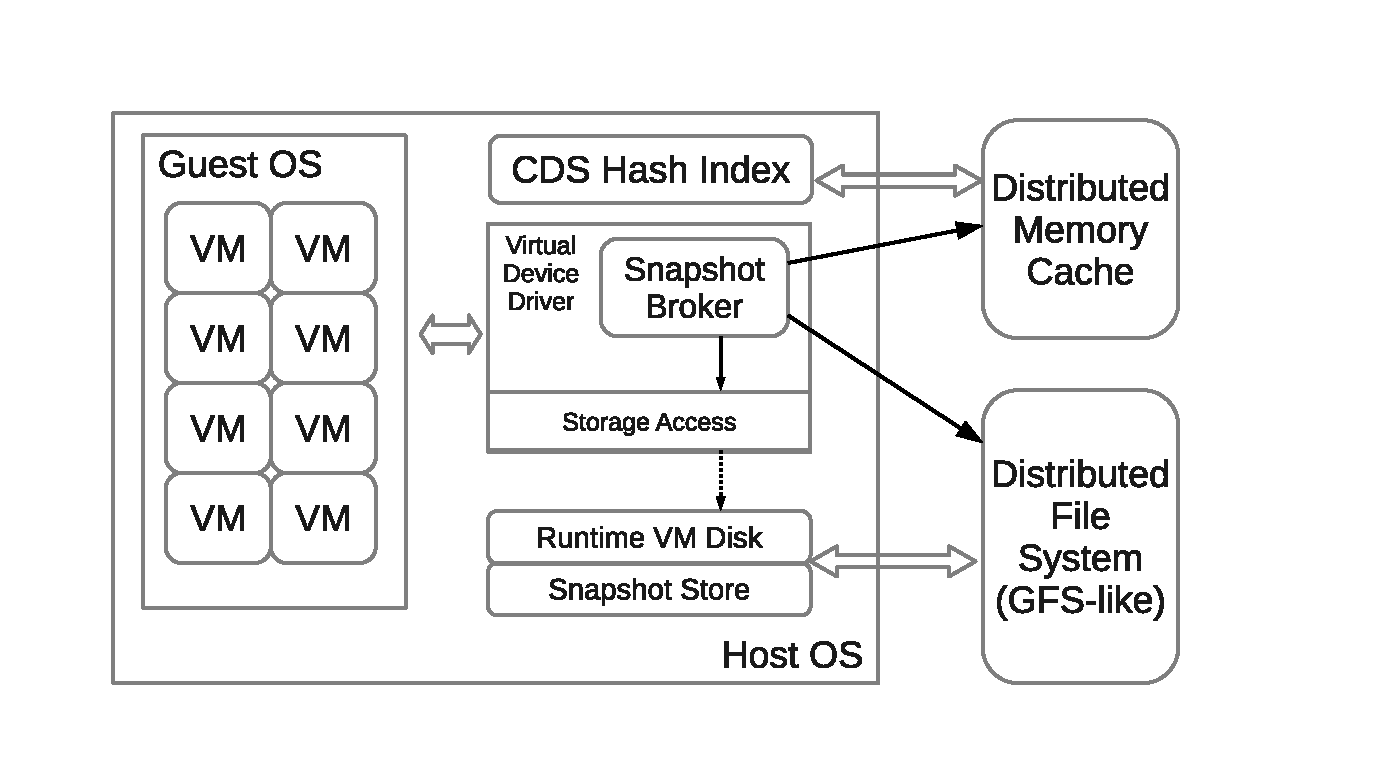
\epsfig{file=images/arch.eps, height=2in, width=2.66in}
  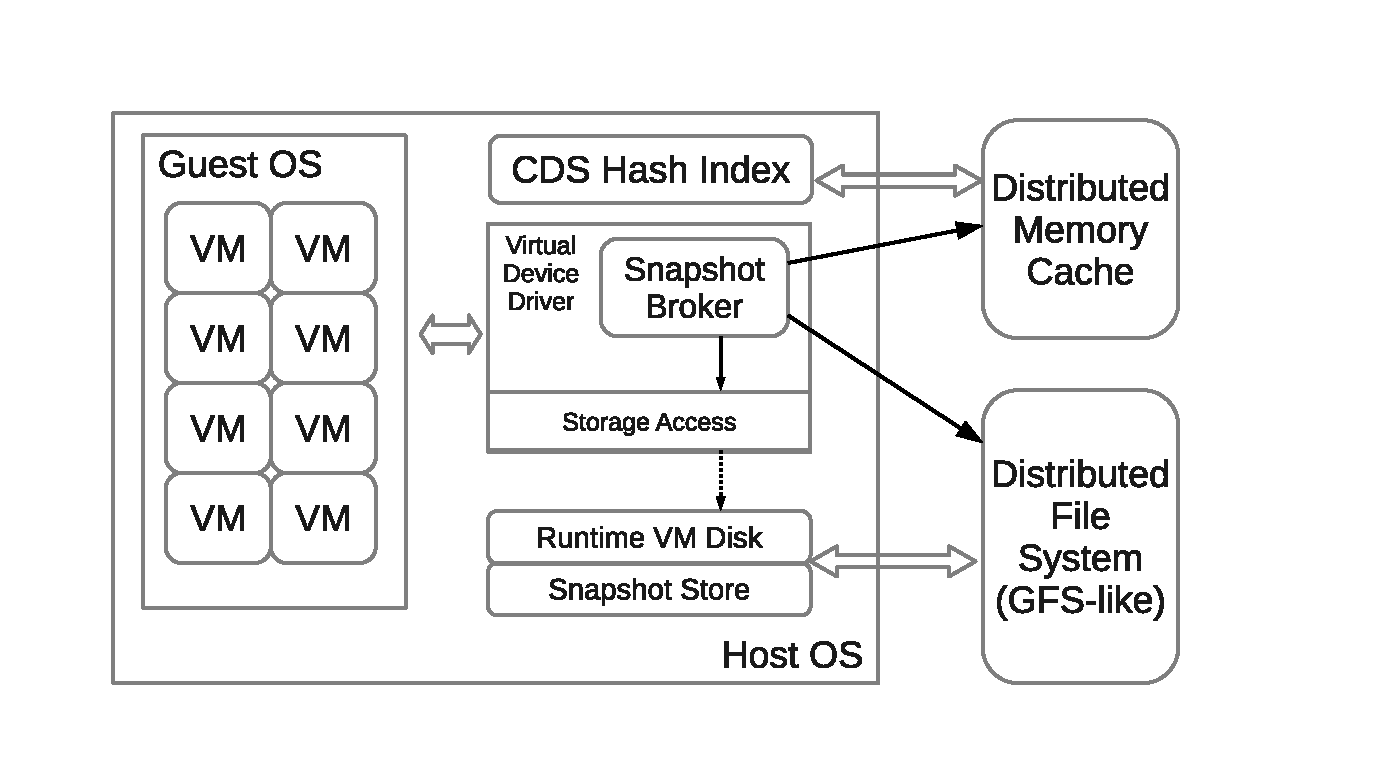
\epsfig{file=images/arch.eps, width=3.9in}
  \caption{Snapshot backup architecture of each node.}
  \label{fig:arch}
\end{figure}

Figure~\ref{fig:arch} shows the architecture view of our snapshot service
at each node. The snapshot broker provides the functional interface for  snapshot backup, access, and deletion.
The inner-VM  deduplication is conducted by the broker to access meta data in the snapshot data store
and we discuss this in details in Section~\ref{sect:innerVM}.
The cross-VM deduplication is conducted by the broker to access 
a common data set (CDS) (will discuss in Section~\ref{sect:crossVM},
whose block hash index is stored in a distributed memory cache. 

\section{VM-centric Snapshot Deduplication}
\label{sect:dedupe}
%snapshot representation

%We use the The deduplication process is first conducted among snapshots within each VM
%and then is conducted across VMs.
%Given the concern that searching duplicates across VMs is a global feature which can affect parallel performance
%and complicate failure management,
%we only eliminate the duplication of a small but popular data set while still maintaining a cost-effective deduplication ratio.
%For this purpose, we exploit the data characteristics of snapshots and collect most popular data.
%Data sharing across VMs is limited within this small data set such that adding replicas for it could enhance fault tolerance

%A deduplication scheme compares the fingerprints of the current snapshot
%with its parent snapshot and also other snapshots in the entire cloud.
%The traditional approach compares all fingerprints and 
%stores one copy for all of a chunk's duplicates.
%We call this as  the VM-oblivious (VO) approach.
Our VC design has the following  objectives: 1)  localizing deduplication while identifying a decent amount of
duplicates among VMs to maintain a competitive deduplication efficiency and simplify snapshot management;
2) Minimizing the number of file system blocks shared among VMs and adding extra replicas for shared blocks.

\comments{
\begin{itemize}
\item
1) Localize the deduplication and data blocking within each VM as much as possible so 
that any failure of a file system block mainly affects the associated VM.
Localizing the snapshot data deduplication within a VM
improves the system by increasing data independence between different VM backups,
simplifying snapshot management and statistics collection,
and facilitating parallel execution of snapshot operations.
\item
2) Maintain a competitive deduplication efficiency while being resource-friendly to other
existing cloud services.
Cross-VM duplication can be desirable since  there are many cloud images
use widely-used software and libraries and their data blocks are duplicate. 
As the result, different VMs tend to backup large amount of highly similar data.
\item
\end{itemize}
}
\subsection{Key VM-centric  Strategies}
\label{sect:vc-strategies}

%Inner-VM duplication can be very effective within VM's snapshots. There
%are typically a large number of duplicates existing among the snapshots
%for a single VM.  

%Our multi-level pipeline process can minimize 
%the cost of deduplication while maximize the its efficiency at each level,
%and it is parallel since each segment is processed independently.

%Our VC differentiates duplicates within a VM and cross VMs,
%and conducts \textit{Inner-VM} and \textit{cross-VM} detection separately. 

\begin{itemize}
\item \textbf{VM-specific local duplicate search within similar segments.}
We start with the standard dirty bit approach in a coarse grain segment level.
In our implementation with Xen at an Alibaba platform, the segment size is 2MB
and  the device driver is extended to support  changed block tracking. 
Since every write for a segment will touch a dirty bit, the device driver maintains dirty bits in memory
and cannot afford a small segment  size.
%Xen doesn't directly support it, However, their open-source 
%architecture allows anyone to extend 
%and use the  Xen virtual device driver to implement a feature called ``changed block tracking''
%for the storage device and the dirty bit setting is maintained in a coarse grain level we call it a segment.
It should be noted that dirtybit tracking is supported or can be easily implemented in 
major virtualization solution vendors. For example,
%(VMware, Xen, Microsoft).  
%VMware support it directly; 
the VMWare hypervisor has an API to let external backup applications know 
the changed areas since last backup. 
%We implement dirty bit tracking this way in Alibaba's platform.  
The Microsoft SDK provides an API that allows external applications to monitor 
the VM's I/O traffic and implement  the changed block tracking feature.

Since the best deduplication uses a nonuniform chunk size 
in the average of 4K or 8K~\cite{??},  
%This allows the system to achieve deduplication even when there are insertions/deletions which would
%affect many fixed-size chunks.
we conduct additional local inner-VM deduplication by comparing
dirty segment's chunk fingerprints to similar segments from its parent snapshot. 
For every segment, the minimum value of all its chunk fingerprints is computed during backup
and is recorded in the snapshot recipe.
When we are processing a dirty segment,
we can easily find similar segments from the
parent snapshot recipe and load their segment recipes. Then 
given a set of data chunks within a dirty segement,  we compare  these chunk fingerprints
with those in similar segments.  
For example, with a 2MB segment, there are about 500 fingerprints to compare.
The amount of memory for maintaining those fingerprints in similar segment s is small, as we only
load one dirty segment at a time.


%If we use 4KB in level-1, then such a level-1 should have similar dedup efficiency 
%as the current level-1 and level-2 combined, because finally they equal to comparing  
%parent snapshot at 4KB granularity.
%
%However, at level-3 things are different. If we use 4KB fix-size block uniformly, it would be harder for different VM to share data through PDS, because there is no guarantee that the location of duplicate data on different VM disks are always aligned at 4KB boundary. For example, if two VMs each has a copy of duplicate data, but they are not aligned, then we won't be able to detect them. Our study at the current small data set has shown that using 4KB fix-size block will make PDS method less efficient by nearly 10%. Over the long time, more and more OS variations will co-exist in the cluster, making this 4KB fix-size approach inefficient in reducing duplicate data across VMs.

%\item \textit{Level 2  Chunk fingerprint comparison.}
%If a segment is modified, we perform fine-grained deduplication 
%by comparing the fingerprints of its chunks to the same segment's recipe in the previous snapshot,
%thus eliminate partial data duplication within the segment.
%\end{itemize}
%
%In general, operations at level 1 have almost no cost and most of unmodified data are filtered here. 
%To process a dirty segment at level 2, 
%there requires no more than one DFS access to load the segment recipe from previous snapshot,
%and a tiny amount of memory to hold it in main memory.

\item \textbf{Cross-VM deduplication with popular chunks and replication support}
This step accomplishes the standard global fingerprint  comparison as conducted
in the previous work~\cite{??}.
One key observation is that the inner deduplication has removed many of the duplicates.
There are fewer deduplication opportunities across VMs while the memory and network
consumption for global comparison is more expensive.
Thus our approximation is that the global fingerprint comparison only searches for the top $k$
most popular items. This dataset is called PDS (common data set). 
%Since duplicate sharing patterns among  VM follows a zip-like distribution,  
The popularity of a chunk is the number  of data chunks  from different VMs
that are duplicates of this chunk after the inner VM deduplication.
This number can be computed periodically on a weekly basis.
Once the popularity of all data chunks is collected, the system only maintains the top $k$
most popular chunk signatures in a distributed shared memory.  
%For cross-VM comparison, we only store  top $k$ items and $k$ is chosen to be relatively small.

Since $k$ is relatively small and these top $k$ chunks are shared among multiple VMs, 
we can afford to provide extra replicas for these popular chunks to enhance the fault resilience.
%We will provide an analysis of the space need and fault tolerance in the next subsection.

\item \textbf{VM-centric file system block management.}
When a chunk is not detected as a duplicate to any existing chunk, this chunk will be written
to the file system. Since the backend file system typically uses a large block size such as 64MB, each VM will 
accumulate small local chunks. We manage this accumulation process using an append-store  scheme
and discuss this in details in Section~\ref{sect:arch}.
The system allows all machines conduct the backup in parallel in different machines, and each machine
conducts the backup of one VM at a time, and thus only requires a write  buffer for one VM.

PDS chunks are stored in a separate append-store instance. In this way, each
file block for non-PDS chunks is associated with one VM and does not contain
any PDS chunks. 
\end{itemize}

We have not  adopted the  sampled index~\cite{Guo2011} 
for  popular data chunks and  this is because sampling requires the use of prefetching to be effective.
%For a small set of popular data chunks, the prefetching strategy
%used In the sampled index will not work well because 
For the data sets we have tested, the spatial locality is limited among popular
data chunks and  on average the number of consecutive data chunks is 7 among popular chinks, which is not sufficient.
%to be effective for index sampling.


 \subsection{Impact on deduplication efficiency}
%VM-oriented Fault Isolation}
%Our objective for fault isolation is to minimize the number of VMs affected when there are failures
%in the cluster.  
%The inner-VM deduplication does not depend on any global service and the comparison
%for each VM is localized within the parent and the current snapshot.
%Lack of data dependence between VMs brings 
%Our analysis below will show that the algorithm can still deliver competitive
%deduplication efficiency after making these approximations.
%With cross-VM deduplication, shared data chunks
%create an artificial dependence  among VMs. 
%Thus we only maintain the index for the most popular chunks to reduce the inter-VM dependence
%while still accomplishing competitive deduplication efficiency. 

%The management for popular data chunks contains two aspects.



We analyze how the choice of value  $k$ impacts the deduplication efficiency.
%It also  compares the  fault resilience of our VM-centric deduplication approach with a standand approach using 
%global deduplication.
%\subsubsection{Impact of PDS deduplication}
The analysis is based on the characteristics  of the VM snapshot traces
studied from  Alibaba's production user data.
Our previous study shows that the popularity of data chunks after inner VM deduplication follows 
a Zipf-like distribution\cite{zipf} and its
exponent $\alpha$ is ranged between 0.65  and  0.7.~\cite{ieeecloud}. 
%As a result, it can be proved that deduplication efficiency of PDS index is scalable:
Table~\ref{tab:symbol} lists parameters used in this analysis.


\begin{figure}
\centering
%\epsfig{file=log-log.disk,width=3in}
%source ../vm_snapshot_sim/images/log-log.disk.eps
 \includegraphics[width=3in]{figures/log-log-disk}
\caption{Duplicate frequency versus  chunk ranking in a log scale.}
\label{fig:Datazipf}
\end{figure}

\begin{table}[ht]
\centering
\begin{tabular}{|p{1.25cm}|p{6.5cm}|}
\hline
$k$ &  the number of top most popular chunks\\ 
\hline
$c$ &  the total amount of data chunks\\ 
\hline
$c_u$ &  the total amount of unique fingerprints after inner VM  deduplication\\
\hline
$f_i$ &  the frequency for the $i$th most popular fingerprint\\
\hline
$\delta$ &  the percentage of duplicates detected in inner VM deduplication\\
\hline
$\sigma$ &  the number of unique non-PDS chunks over  the number of the PDS chunks.\\
\hline
$p$ & the number of machines in the cluster\\
\hline
$V$ & the number of VMs on each machine\\
\hline
$D$ & the amount of unique data on each machine\\
\hline
$C$ & the average data chunk size. Our setting is  4K.\\
\hline
$s$ & the average size of file system blocks in the distributed file system. The default is  64MB.\\
\hline
$m$ & memory size on each node used by VC\\ 
\hline
$E$ & the size of an popular data index entry\\
\hline
$N_1$ & the average number  of non-PDS file system blocks  in a VM\\
\hline
$N_2$ & the average number  of PDS file system blocks  in a VM\\
\hline
$N_o$ & the average number  of file system blocks  in a VM for VO\\
\hline
\end{tabular}
\caption{Modeling  parameters and symbols.}
\label{tab:symbol}
\end{table}

{\it [Need to find a place to put these numbers in: Total number of chunks 
in 350 snapshots: 1,546,635,485. 
Total number of chunks after localized dedup: 283,121,924. Total number of unique chunks: 87,692,682.]}

As summarized in Table~\ref{tab:symbol},
let $c$ be the total number of data chunks. 
$c_u$ be the total number of fingerprints 
in the global index after complete deduplication, and
$f_i$ be the frequency for the $i$th most popular fingerprint. 
By Zipf-like distribution, $f_i = \frac{f_1}{i^\alpha}.$
Since $ \sum_{i=1}^{c_u}f_i = c$,
\[
f_1 \sum_{i=1}^{c_u}\frac{1}{i^\alpha} = c.
\]
Given $\alpha <1$, $f_1$ can be approximated with integration:
\begin{equation}
f_1=\frac{c(1-\alpha)}{c_u^{1-\alpha}}.
\end{equation}

%We define deduplication efficiency $e$ to be the proportion of raw data that can be deduplicated,
%In complete deduplication scenario, it deduplication efficiency $e_c$ is:
%\begin{equation}
%e_c = \frac{b-b_u}{b} = 1 - \frac{b_u}{b}
%\end{equation}

The  $k$ most popular fingerprints can cover the following number of chunks after inner VM 
deduplication:
\[
f_1 \sum_{i=1}^{k}\frac{1}{i^\alpha} \approx  
f_1 \int_{1}^{k}\frac{1}{x^\alpha} dx  \approx  f_1\frac{  k^{1-\alpha}} {1-\alpha}.
\]

Deduplication efficiency of VC using top $k$ popular chunks
is the percentage of duplicates that can be detected:  
\begin{equation}
%\begin{split}
%e_k &= 
\frac{ c(1-\delta) + f_1\frac{  k^{1-\alpha}} {1-\alpha}} 
{c(1-\delta)  + \delta c - c_u }\\
= 
\frac{ (1-\delta) + \delta  (\frac{k}{c_u})^{1-\alpha}}
{ 1- \frac{c_u}{c} }.
%\end{split}
\end{equation}


%\begin{equation}
%\begin{split}
%e_k &= (\sum_{i=1}^{k}C_i - k)/{b} = (b * \frac{1-\alpha}{b_u^{1-\alpha}} * \sum_{i=1}^{k}\frac{1}{i^\alpha} - k)/b \\
%&\approx \frac{b*\frac{1-\alpha}{b_u^{1-\alpha}}*\frac{k^{1-alpha}}{1-\alpha} - k}{b}
%&\approx (\frac{k}{b_u})^{1-\alpha} - \frac{k}{b} \approx (\frac{k}{b_u})^{1-\alpha},\; (since\; k \ll b)
%\end{split}
%\end{equation}

% For the Zipf-like distribution, an approximation to the sum of the first $n$ 
% elements of the distribution can be derived as follows:
% \begin{equation}
% \sum_{i=1}^{n}\frac{1}{i^\alpha}\approx \int_{1}^{n}\frac{1}{x^\alpha}\mathrm{d}x=\frac{x^{1-\alpha}}{1-\alpha}=\frac{n^{1-\alpha}}{1-\alpha}\;  for\;  \alpha<1
% \end{equation}

% So the cumulative distribution function for a PDS holding top $S_c$ fingerprints
% of global index with size $S_g$ is:

% \begin{equation}
%   E = (S_c / S_g)^{1-\alpha} \;  for\;  \alpha<1
% \end{equation}

%[Describe the dedup efficiency model in detail]
Let $p$ be the number of physical machines in the cluster, $m$ be the memory on each node used by the popular
index, $E$ be the size of an index entry,
$D$ be the amount of unique data on each physical machine, and 
$C$ be the average chunks size. We store the popular index using a distributed shared memory hashtable
such as MemCacheD.  Then $k$ and $c_u$ can be expressed as:
$
k = p*m/E$, and $c_u = p*D/E.
$

The overall deduplication efficiency of VC is
\[
\frac{ (1-\delta) + \delta (\frac{m*C}{D*E})^{1-\alpha}}
{ 1- \frac{c_u}{c} }.
\]
where $(\frac{m*C}{D*E})^{1-\alpha}$ represents the percentage of the remaining
chunks detected as duplicates after inner VM deduplication.
Figure~\ref{fig:cds-coverage} shows measured PDS coverage in our 35 VM dataset.
You can see from the graph that the coverage actually increases as the data size
increases, which indicates that $\alpha$ increases with the data size (a
fixed-$\alpha$ model would predict constant coverage). This makes the PDS even
more effective, as the coverage of the PDS increases as more data is added.
%Then the deduplication efficiency of PDS approach using top k most popular fingerprints is:
%\begin{equation}
%  e_k = (\frac{m*B}{F*D})^{1-\alpha}
%\end{equation}


% is mainly affected by the its memory usage,
%and the Zipf-like distribution parameter $\alpha$.
%From the memory usage perspective, the more memory we give to PDS index, the more duplicates it can found.
%From the data characteristics perspective, if the system tends to backup arbitrarily random data, 
%$\alpha$ would be small and thus PDS approach would not be effective. But in a VM cluster all VMs
%have a large portion of similar data, thus leading to a bigger $\alpha$. The more VM join the cluster,
%the better deduplication efficiency our PDS deduplication approach will have.




\comments{
Since $B$, $D$ and $F$ are environment constants, the deduplication efficiency of PDS is mainly affected by its memory usage,
and the Zipf-like distribution parameter $\alpha$.
From the memory usage perspective, the more memory we give to PDS index, the more duplicates it can found.
From the data characteristics perspective, if the system tends to backup arbitrarily random data, 
$\alpha$ would be small and thus PDS approach would not be effective. But in a VM cluster all VMs
have a large portion of similar data, thus leading to a bigger $\alpha$. The more VM join the cluster,
the better deduplication efficiency our PDS deduplication approach will have.
}

\comments{ %this table is superceded by the graph below it
\begin{table}
    \begin{tabular}{llll}
    Data size (GB) & 1\%    & 2\%    & 4\%    \\
    14.6           & 18.6\% & 22.1\% & 31.4\% \\
    28.1           & 19.5\% & 26.2\% & 38.8\% \\
    44.2           & 21.7\% & 26.5\% & 36\%   \\
    61.6           & 23.2\% & 32.9\% & 35\%   \\
    74.2           & 23.6\% & 33.6\% & 37.5\% \\
    \end{tabular}
    \caption{Deduplication effectiveness of top k\% of global index}
    \label{tab:cds}
\end{table}
}


\begin{figure}[ht]
  \centering
    \begin{tikzpicture}
            \begin{axis}[
            %title={PDS Coverage},
            width=\linewidth,
            height=0.7\linewidth,
            cycle multi list={
                mline\nextlist
                [3 of]mmark*\nextlist
            },
            %cycle list name=mcolor,
            xlabel={Total num. chunks stored (in billions)},
            ylabel={PDS Coverage (\%)},
            %extra y ticks={4.5,5.5,6.5} %to add extra ticks
            mark options=solid,
            %legend pos=outer north east,
            legend columns=2,
            legend style={
                at={(0.5,-0.2)},
            anchor=north},
            ]
            \addplot table[x expr=\thisrow{InputChunks}/1000000000,y=A1] {figures/cds_coverage.txt};
            \addplot table[x expr=\thisrow{InputChunks}/1000000000,y=A2] {figures/cds_coverage.txt};
            \addplot table[x expr=\thisrow{InputChunks}/1000000000,y=A4] {figures/cds_coverage.txt};
            \addplot table[x expr=\thisrow{InputChunks}/1000000000,y=T1] {figures/cds_coverage.txt};
            \addplot table[x expr=\thisrow{InputChunks}/1000000000,y=T2] {figures/cds_coverage.txt};
            \addplot table[x expr=\thisrow{InputChunks}/1000000000,y=T4] {figures/cds_coverage.txt};
            \legend{Measured ($\sigma=1\%$),Measured ($\sigma=2\%$),Measured ($\sigma=4\%$),Predicted ($\sigma=1\%$),Predicted ($\sigma=2\%$),Predicted ($\sigma=4\%$)};
            \end{axis}
    \end{tikzpicture}
  \caption{fixed-alpha predicted vs. actual PDS coverage as data size increases.}
  \label{fig:cds-coverage}
\end{figure}



As illustrated in Figure~\ref{??},
when the number of machines at each cluster increases, the number of total VMs increases.
Then $k$ increases since more memory is available to host the popular chunks index.
But for each physical machine, the number of VMs remains the same, and thus
$D$ is  a constant. Then  the overall deduplication efficiency of VC remains
a constant.

\section{Append Store}
\label{sect:append}
\subsection{Introduction}
Append Store (AS) is our underlining storage engine for storing snapshot data after deduplication. 
AS is built on top of our highly scalable distributed file system (DFS), 
which is very similar to Google's file system
in a sense that it is optimized for large files and sequential read/append operations.

\subsection{Design considerations}
While scalability has been handled by the DFS, there are still several challenges in 
storing billions of variable-sized small data chunks:
\begin{description}
\item[Locality perseveration] Chunk data must be placed next to each other in the order of their writing sequence,
because reading a snapshot incurs large sequential reads of chunks under their logical sequence in the snapshot.
\item[Flexible referencing] To avoid overwhelming metadata operation capbility of DFS's master, 
we have to group small chunks into large data files in DFS.
However, snapshot deletion brings chunk data deletion, and reclaiming disk space would require many chunks being moved.
If such chunk movement incurs updates of data referencing in snapshot and segment recipes, then the cost of deleting 
a snapshot would be extremely high.
\item[Efficient chunk lookup] The translation from data reference to data location must be very efficient in two ways: 
first, a sorted index is necessary to quickly find the data location in $O(log(n)$ time; 
second, the size of the index must be optimized to minimize its memory footprint and the cost of fetching index. 
\end{description}



\subsection{Architecture}
\begin{figure}[htbp]
  \centering
  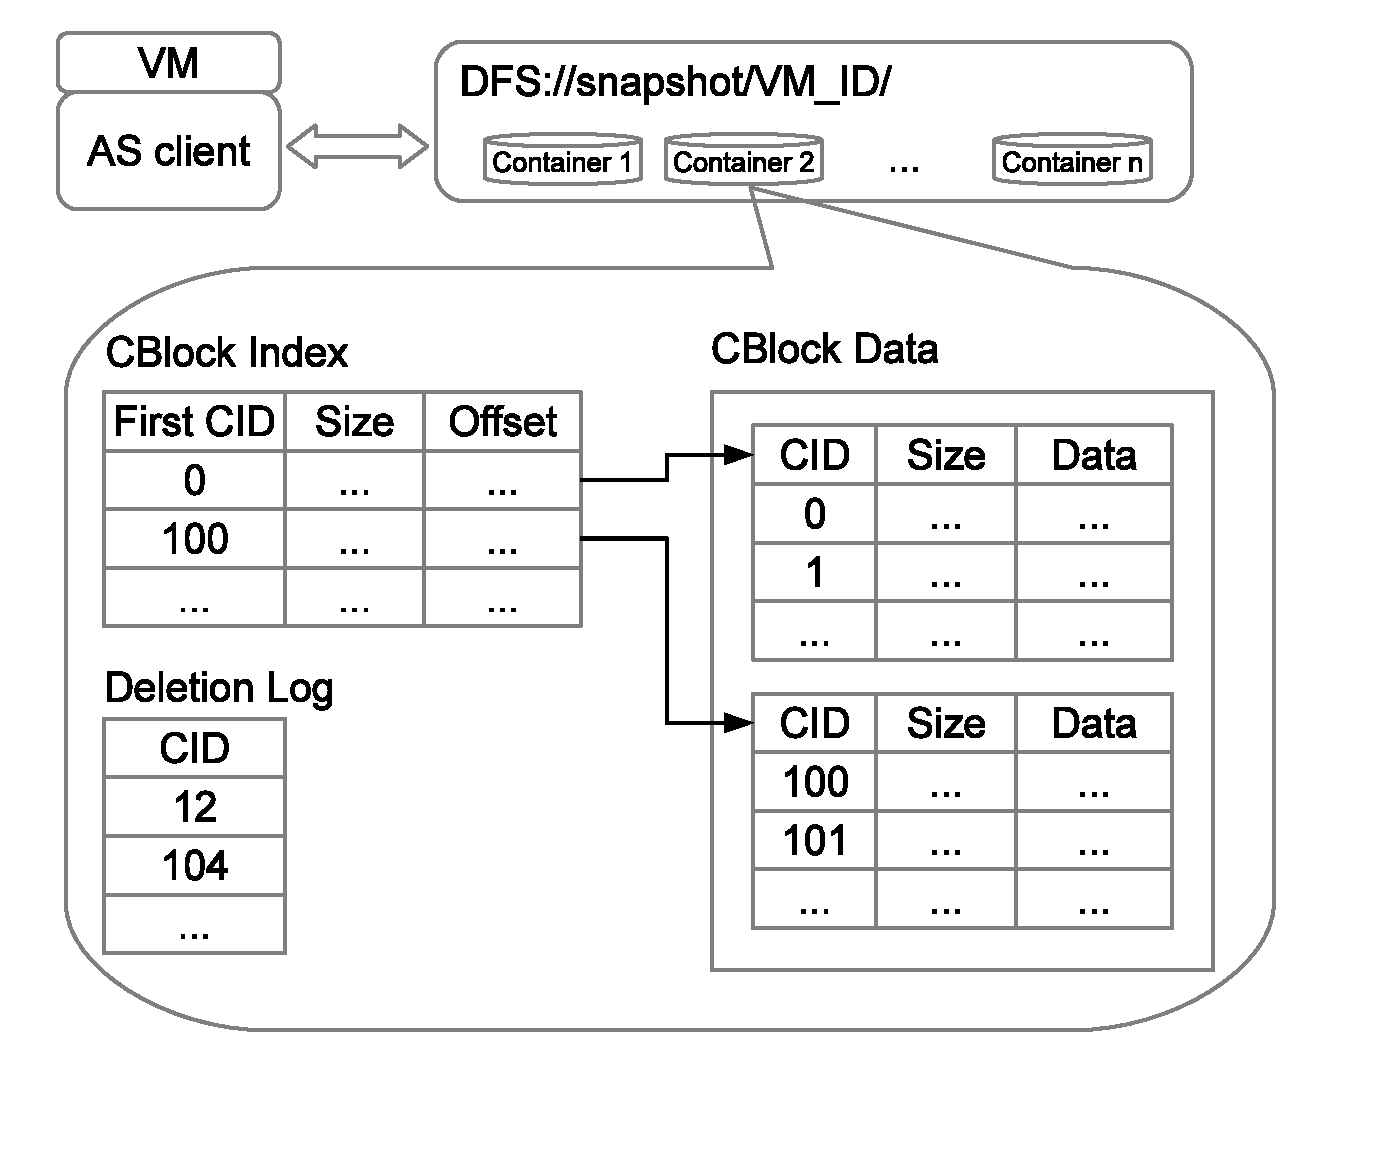
\epsfig{file=images/append_store_arch, width=3.5in}
  \caption{Architecture of Append Store}
  \label{fig:as_arch}
\end{figure}

Append Store supplies three interfaces: {\em get(ref)} accepts a data reference and retrives data, 
{\em put(data)} accepts data and returns a reference to be stored in metadata recipes, 
{\em delete(ref)} 
deletes the data pointed by the reference.
Under the hood, small var-sized data are grouped and stored into larger data containers. Each VM has
its snapshot data stored in its own Append Store, specified by the VM ID. 
We split every Append Store into multiple data containers so that reclaiming the disk space would not 
result in rewriting all the data at the same time.

As shown in Fig.\ref{fig:as_arch}, every data container is represented as three data files in DFS:
the data file holds all the actual data, the index file is responsible for translating data reference
into data locations, and a deletion log file remembers all the deletion requests to the container.

A data reference is composed of two parts: a container ID (2 bytes) and CID (6 bytes).
Append Store assign every piece of data a CID for its internal data referencing. 
When new data is appended, its CID is the current largest CID in that container plus one.
As a result, all the data locations are naturally indexed by this self-incremental CID, 
no extra sorting is needed.

Append Store groups multiple chunk data (i.e., 100) into larger units, called {\em CBlock}.
CBlock is the basic unit for append store's internal read/write/compression.
There is one index entry in the container index corresponding to every CBlock. It keeps the first chunk's CID
in that CBlock, and the CBlock data's size and location.

Using CBlock brings us several advantages: First, the write workload to DFS master is greatly reduced; second, grouping
small chunks gives better compression. Third, reading a CBlock (200 - 600 KB) typically cost the same amount of disk 
seek as reading a 4KB chunk. Finally, this greatly reduces the size of index. Let $m$ be the number of chunks in each
CBlock, then the overall index size is reduced to $1/m$. In our implementation, using $m=100$ reduces the index for
a 1GB container from 10 MB to 100 KB.

\subsection{Operations}
In order to read a chunk data by reference, Append Store client first loads the
container index file specified by the container ID, then search the CBlock index to find the entry that covers the chunk by CID.
After that, it reads the whole CBlock data from DFS, decompress it, seek the exact chunk data specified by CID. 
Finally, the client updates itws internal chunk data cache with the newly loaded contents to anticipate future sequential reads.

Write requests to append store are accumlated. When the number reaches $m$, the AS client forms a CBlock by assigning 
every chunk a CID, compress the CBlock data, and append it to the CBlock data file. Then a new CBlock index entry is appended
to CBlock index.

Append store adopts lazy delete strategy. The deletion requests are appended into every container's deletion log file with the CID of data to be deleted.
CIDs in deletion log are guaranteed to be referenced by nobody and can be safe deleted in future. 
Periodically, snapshot management system asks append store to compact containers in order to reclaim disk space. 
The actual compaction will only take place when the number of deleted items reached $d\%$ of container's capacity. 
During compaction, append store creates a new container (with the same container ID) to replace the 
existing one. This is done by sequentially scan the old container, copying all the chunks that are not 
found in deletion log to the new container, creating new CBlocks and indices. 
However, every chunk's CID is plainly copied rather than re-generated. This does not affect the sorted
order of CIDs in new container, but just leaving holes in CID values. As the result, all data references stored 
in upper level recipes are unaffected, and the data reading process is as efficient as before.

%hard problems

\subsection{Analysis}

Snapshot operation performance analysis:
\begin{table}
    \begin{tabular}{l p{1.5in} l}
        \hline
        Symbol & Description & Measurement \\ \hline
        $N_{seg}$ & Number of segments in the snapshot & ~ \\ [1ex] \\ [-1.5ex]
        $N_{chunk}$ & Number of chunks in one segment & ~ \\ [1ex] \\ [-1.5ex]
        $P_{dirty}$ & Probablity of a segment is dirty & ~ \\ [1ex] \\ [-1.5ex]
        $P_{new}$ & Percentage of new data & ~ \\ [1ex] \\ [-1.5ex]
        $P_{change}$ & Probablity that a chunk is not found in parent snapshot & ~ \\ [1ex] \\ [-1.5ex]
        $P_{in\_PDS}$ & Percentage of chunks in PDS & ~ \\ [1ex] \\ [-1.5ex]
        $T_{scan}$ & Time to scan segment data and caculate content hash & 74 ms \\ [1ex] \\ [-1.5ex]
        $T_{write\_AS}$ & Time of writing a chunk into append store & 0.24 ms \\ [1ex] \\ [-1.5ex]
        $T_{read\_AS}$ & Time of reading a chunk from append store & ~ \\ [1ex] \\ [-1.5ex]
        $T_{read\_chunk}$ & Time of reading a chunk & ~ \\ [1ex] \\ [-1.5ex]
        $T_{check\_PDS}$ & Time of checking PDS & ~ \\ [1ex] \\ [-1.5ex]
        $T_{read\_PDS}$ & Time of reading a chunk data from PDS data store& ~ \\
        \hline
    \end{tabular}
    \caption{List of performance factors}
    \label{tab:as_param}
\end{table}

The overall time of writing a snapshot is:

\begin{dmath}
T_{write} = P_{dirty} * N_{seg} * [max(T_{scan}, T_{read\_AS}) + P_{change} * N_{chunk} * T_{check\_PDS} + P_{new} * N_{chunk} * T_{write\_AS}]
\end{dmath}

The overall time to read a snapshot is:

\begin{dmath}
T_{read} = N_{seg} * {T_{read\_AS} + N_{chunks} * [P_{in\_PDS} * T_{read_PDS} + (1 - P_{in\_PDS}) * T_{read\_chunk}]}
\end{dmath}

Average time of reading a chunk:

\begin{dmath}
T_{read\_chunk} = P_{in\_PDS} * T_{read\_PDS} + (1 - P_{in\_PDS}) * T_{read\_AS}
\end{dmath}

Time of reading append store:

\begin{dmath}
T_{read\_AS} = 0 * P_{in\_cache} + (1 - P_{in\_cache} ) * T_{load\_CBlock}
\end{dmath}

\section{Deletion}
In a mature VM cluster, snapshot deletions are as frequent as snapshot creations.
Our system adopts lazy delete strategy so that all snapshot deletions are scheduled
in the backup time window at midnight. 
Therefore, snapshot deletions must be fast enough to fit in time window and
efficient enough to satisfy our resource constraints.
However, there is no simple solution can achieve these goals with high reliability.
In Aliyun's cloud, we use a {\em fuzzy deletion} method to trade deletion accuracy for
speed and resource usage. This method tolerates a tiny percentage of storage leakage
to make the deletion operation faster and efficient by an order of magnitude,
yet we still adopt an slow but accurate deletion method to fix such leakage in the long-term.
Our hybrid deletion strategy, using fuzzy deletion regularly and accurate deletion periodically,
accomplishs our speed, resource usage and relibility goals very well.

% \subsection{Challenges}
% Contrary to a traditional backup system, a dedupe system shares data among files by default. 
% Reference management is necessary to keep track of chunk usage and reclaim freed space. 
% In addition to scalability and speed, reliability is another challenge for reference management. 
% If a chunk gets freed while it is still referenced by snapshots, data loss occurs and files cannot be restored. 
% On the other hand, if a chunk is referenced when it is actually no longer in use, it causes storage leakage.

% Reference counting, while being simple, suffers from low reliability especially in our distributed environment, 
% because it is vulnerable to lost or repeated updates: when errors occur some chunks maybe updated and some may not. 
% Complicated transaction rollback logic is required to make reference counts consistent. Moreover, 
% there is almost no way to verify if the reference count is correct or not in a large dynamic system. 
% In real deployments, where data integrity and recoverability directly affect product reputation, simple reference counting is unsatisfactory.

% Mark-and-sweep is generally a better solution. During the mark phase, all snapshot recipes are traversed so as to mark the used chunks. 
% In the sweep phase all chunks are swept and unmarked chunks are reclaimed. 
% This approach is very resilient to errors: at any time the process can simply be restarted with no negative side effects. 
% Scalability, however, is an issue. {\em needs to explain its resource usage}


\subsection{Approximate Deletion}
\begin{figure}[htbp]
  \centering
  \epsfig{file=images/deletion.png, width=3.5in}
  \caption{Approximate deletion}
  \label{fig:deletion_flow}
\end{figure}

We design approximate deletion to fast identify unused data in the append store.
Instead of scanning the whold append store, it uses a Bloom filter to check 
if a data are still referenced by living snapshots. However, there is a small false-positive probility which
would indetify unused data as in use, i.e., storage leakage.
The following steps would take place during an approximate deletion:

\begin{enumerate}
\item {\bf Creating Bloom filter} Scan all the living snapshot recipess and their segment recipes,
for every reference pointing to append store, add it to the Bloom filter.
\item {\bf Check existance} For every data reference in the deleted snapshot recipe and its segment recipes,
check the existance of that data reference in Bloom filter. If not found, it is safe to delete that piece of data from append store
because no living snapshots has referenced it.
\end{enumerate}

The overall time of running a approximate deletion for one snapshot deletion would be scanning
all the living snapshots and deleted snapshots, since operations on the in-memory Bloom filter can be done in
parallel and is much faster than loading recipes from DFS:
\begin{equation}
T = (N_{SS} + 1) * T_{scan\_recipes}
\end{equation}
 
Using the example and analysis in previous section, this approximate deletion can be done in 5 minutes. 
Memory usage of the Bloom filter depends on its false-positive probility $P_{bl}$,
when set $P_{bl}$ to 0.01, the memory footprint of approximate deletion is about 15 MB.

The design goal of approximate deletion is to reduce the frequency of running accurate deletion.
For one VM's snapshots, let $D_{leakage}$ be the amount of storage leakage, $D_{del}$ be the average amount of data
to be deleted in one snapshot deletion, 
then we have:
\begin{equation}
D_{leakage} = N_{approximate} * P_{bl} * D_{del}
\end{equation}
where $N_{approximate}$ is the number of runs of approximate deletion. 
An accurate deletion is triggered to fix the storage leakage
when $D_{leakage}/D_{del}$ is accmulated to exceed certain threshold $T$:
\begin{equation}
D_{leakage} / D_{del} = N_{approximate} * P_{bl} > T \Rightarrow N_{approximate} > T/P_{bl}
\end{equation}
Therefore, when $P_{bl} = 0.01$ and $T=1$, 
there would be a run of accurate deletion for every $T/P_{bl} = 100$ runs of approximate deletion.
On a machine that hosts 20 VMs and each VM deletes snapshot daily, there would be less than
one accurate deletion scheduled per day.

\subsection{Accurate Deletion}
Our accurate deletion uses mark-and-sweep to find all the unused chunks in a VM's append store.
The following steps would take place during an accurate deletion:

\begin{enumerate}
\item Scan all the containers. For each container, extract full list of existing data references and allocate a bitmap. 
(Notice this list is self sorted.)
\item Scan all the snapshot recipes and segment recipes. For every data reference pointing to append store,
find it in the above lists and mark the corresponding position in bitmaps.
\item Scan the bitmaps, for every bit that are not marked, tell append store the corresponding data reference can be deleted.
\end{enumerate}

Although accurate deletion guarantees reliability and correctness, its speed and resource usage are big problems to our VM cloud.
Let $T_{scan\_AS}$ be the time to scan the VM's append store, $T_{scan\_recipes}$ be the time to scan one snapshot recipe
and its segment recipes, $T_{mark}$ be the time of finding a data reference in the list and mark bitmap, 
$N_{SS}$ be the number of snapshots and $N_c$ be the number of chunks in one snapshot.
The overall time of running an accurate deletion for one VM is:
\begin{equation}
T = T_{scan\_AS} + N_{SS} * T_{scan\_recipes} + N_{SS} * N_c * T_{mark}
\end{equation}

For a virtual disk that has 10 snapshots, 50 GB of data in the append store, $T_{scan\_AS}$ would have cost half an hour already.
In addition, scanning recipes of 10 snapshots cost another 5 minutes.
Furthermore, maintaining the full lists of data references and bitmaps costs about 100 MB of memory. Having tens of VMs
co-lived in one physical machine and deleting snapshot on a daily basis, 
it's infeasible to run accurate deletion as frequent as snapshot deletions.

\subsection{Discussion}


\section{Design Overview}
%[describe what is going to be presented in this section]
We start by analyzing the main features in the design of our system.
We first present its architecture,
then introduce the two major contributions: the colocated deduplication 
scheme and the snapshot deletion strategy.
\subsection{Architecture}
%[describe the cloud environment]
Our architecture, as shown in figure.\ref{fig:arch}, is built on top of 
Alibaba's platform which is the largest cloud service provider in China. 
A typical VM cluster in our cloud environment
consists of from hundreds to thousands of physical machines, each of which can
host tens of xen-based\cite{Barham2003} VMs.
Alibaba's cloud platform provides a hadoop-like infrastructure, 
which includes several highly scalable distributed service:
\begin{description}
\item[Distributed file system] This is a scalable distributed file system (DFS) being optimized for many large and sequential reads or appends. DFS holds the responsibility of managing physical disk storage
in the cloud. All data needed for VM services, such as virtual disk images used by runtime VMs,
and snapshot data for backup purposes, reside in this distributed file system. 
%\item[KV]: a distributed key-value store for managing structured data.
%\item[MapReduce]: a distributed data processing framework supports Map-Reduce\cite{Dean2004}.
\item[Distributed memory cache]: A distributed memory object caching system helps us to hold the fingerprints of those popular data blocks for deduplication inqueries. 
\end{description}
In addition, our implementation also uses MapReduce to facilitate the offline
data processing, and stores a small amount of snapshot metadata in a 
BigTable-like persistent key-value store. 

%[describe the benefits of using mature cloud technologies]
In general, our snapshot system and the virtual machine management service 
rely on these fundamental cloud services
to be functional. Such a colocated deduplication architecture allow us 
to enjoy the benefits from these mature technologies 
such as load balancing, scalability, and fault tolerancy.
Moreover, all the above cloud services can easily find their open-source counterparts,
which improves the generality of our architecture and deduplication scheme.

{\bf Snapshot Representation}
The virtual device driver uses a bitmap to track the changes 
that have been made to virtual disk.
Every bit in the bitmap represents a fix-sized (2MB) region called \textit{segment}, indicates whether the segment
is modified since last backup. Hence we could treat segment as the basic unit 
in snapshot backup similar to
file in normal backup: a snapshot could share a segment with previous snapshot it is not changed. 
Moreover, we break 
segments into var-sized chunks (average 4KB) using content-based chunking algorithm,
which brings the opportunity of fine-grained deduplication by
allowing data sharing between segments.

\begin{figure}[htbp]
  \centering
  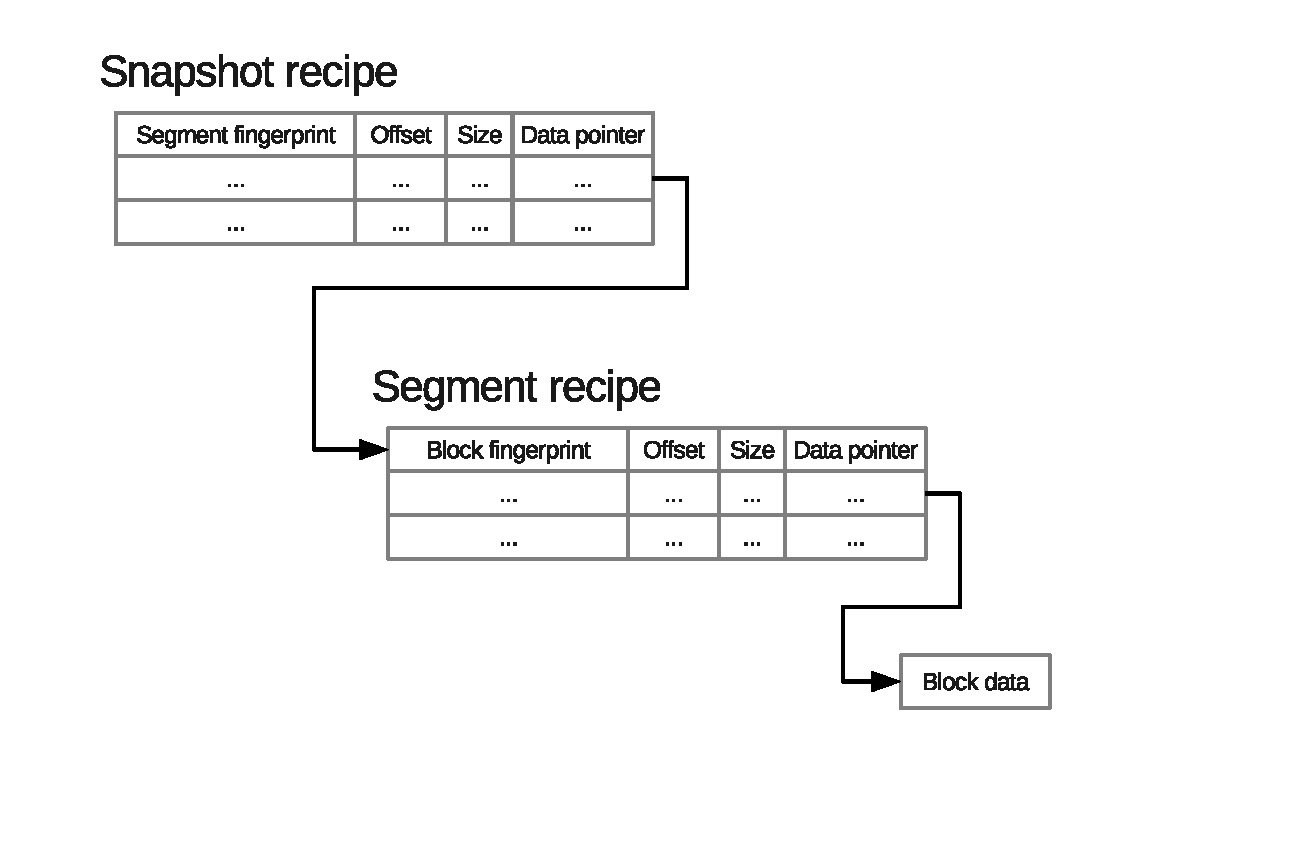
\epsfig{file=images/snapshot_representation.pdf, width=3.7in}
  \caption{An example of snapshot representation.}
  \label{fig:snapshot_rep}
\end{figure}
As a result, the representation of each snapshot is designed as a two-level index data structure 
in the form of a hierarchical directed acyclic graph as shown in Figure \ref{fig:snapshot_rep}.
A snapshot recipe contains a list of segments, each of which is represented as a segment recipe
that holds the meatdata of its chunks. We choose this two-level structure because in practice we
observe that during each backup period only a small amount of VM data are added or modified. 
As the result, even the metadata of two snapshots can be highly similar, 
thus aggregating a large number of chunks as one segment can significantly reduce the space cost of snapshot metadata.
Furthermore, instead of using variables-sized segments, we use a dirty bit to capture the change status of fix-sized
segments which greatly ease the segment-level deduplication.

In both two kind of recipes, 
they do not include the actual data but only have
 references point to the data which are either stored in append store or CDS.
In our implementation the data reference is a 8 bytes field which is either an 
ASID (discuss in \ref{sect:append}) or an offset of an additional flag indicates
the location of CDS data.

\begin{figure}
    \centering
    \subfigure[Node architecture from VM point of view]
    {
        \includegraphics[width=3in]{images/socc_arch_vm.pdf}
        \label{fig:arch_vm}
    }
    \\
    \subfigure[Cluster architecture]
    {
        \includegraphics[width=3in]{images/socc_arch_cluster.pdf}
        \label{fig:arch_cluster}
    }
    \caption{System architecture}
    \label{fig:arch}
\end{figure}

%[describe the architecture frm node side]
{\bf Node Architecuture} 
Our node-side architecture, depicted in figure.\ref{fig:arch_vm}, consists of
two main entities: a virtual block device driver, and a snapshot deduplication component.

%[brief the virtual device driver]
One physical node hosts tens of VMs, each of which access its virtual machine disk image through the
virtual block device driver (called TapDisk\cite{Warfield2005} in Xen).
This driver maintains a map of dirty-bits to record
the change status of every fix-size segment of the virtual disk. 
When the VM issue a disk write, the bits coresponding to the segments that covers 
the modified disk region are set, thus letting snapshot deduplication component knows these
segments must be checked during snapshot backup. After the snapshot backup is finished, 
snapshot deduplication component acknowledges the driver to resume the dirty-bits map to
a clean state.

%[brief the snapshot deduplication]
The snapshot deduplication component consists of the chunking and deduplication 
logic of our snapshot storage system. We choose 

It contains an append store client which provides facilities to manage stored snapshot data, and a CDS client to support CDS index access. We will further discuss our deduplication scheme in section\ref{sec:dedup}.

%[describe the arch from cluster side]
{\bf Cluster Architecture}

%[describe the data structure in underlying storage]
{\bf Append Store}
Append Store (AS) is our underlining storage engine for storing snapshot data after deduplication. 
AS is built on top of our highly scalable distributed file system (DFS), 
which is very similar to Google's file system
in a sense that it is optimized for large files and sequential read/append operations.

\begin{figure}[htbp]
  \centering
  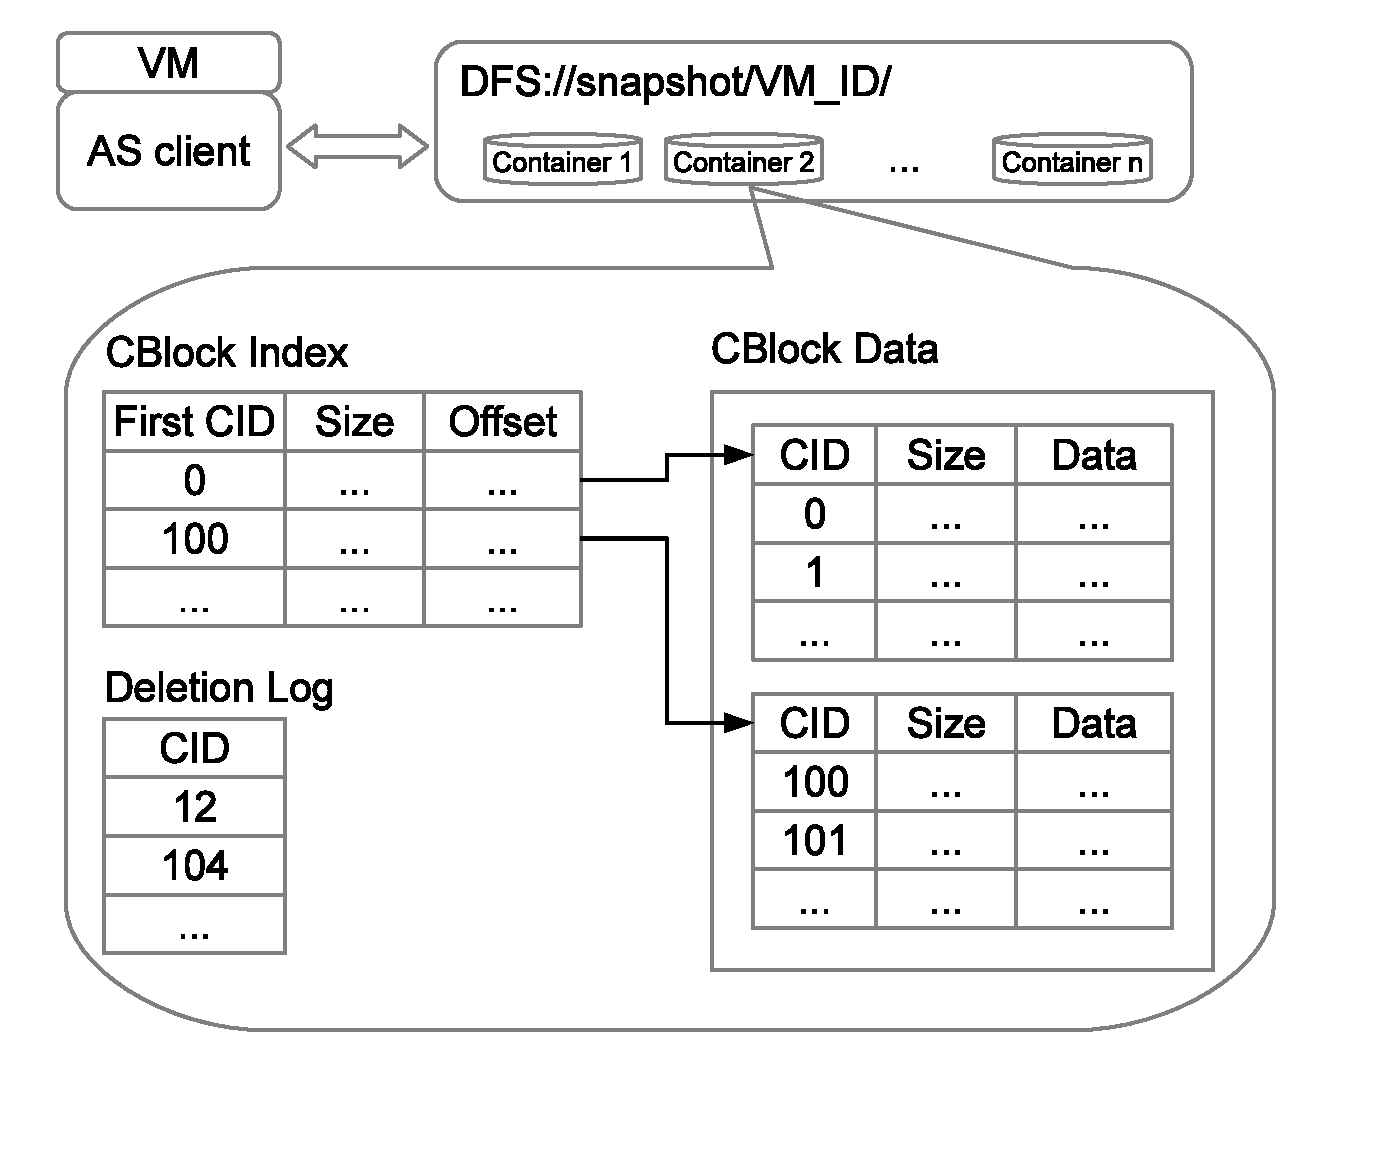
\epsfig{file=images/append_store_arch.pdf, width=3.5in}
  \caption{Architecture of Append Store}
  \label{fig:as_arch}
\end{figure}

Append Store supplies three interfaces: {\em get(ref)} accepts a data reference and retrives data, 
{\em put(data)} accepts data and returns a reference to be stored in metadata recipes, 
{\em delete(ref)} 
deletes the data pointed by the reference.
Under the hood, small var-sized data are grouped and stored into larger data containers. Each VM has
its snapshot data stored in its own Append Store, specified by the VM ID. 
We split every Append Store into multiple data containers so that reclaiming the disk space would not 
result in rewriting all the data at the same time.

As shown in Fig.\ref{fig:as_arch}, every data container is represented as three data files in DFS:
the data file holds all the actual data, the index file is responsible for translating data reference
into data locations, and a deletion log file remembers all the deletion requests to the container.

A data reference is composed of two parts: a container ID (2 bytes) and CID (6 bytes).
Append Store assign every piece of data a CID for its internal data referencing. 
When new data is appended, its CID is the current largest CID in that container plus one.
As a result, all the data locations are naturally indexed by this self-incremental CID, 
no extra sorting is needed.

Append Store groups multiple chunk data (i.e., 100) into larger units, called {\em CBlock}.
CBlock is the basic unit for append store's internal read/write/compression.
There is one index entry in the container index corresponding to every CBlock. It keeps the first chunk's CID
in that CBlock, and the CBlock data's size and location.

Using CBlock brings us several advantages: First, the write workload to DFS master is greatly reduced; second, grouping
small chunks gives better compression. Third, reading a CBlock (200 - 600 KB) typically cost the same amount of disk 
seek as reading a 4KB chunk. Finally, this greatly reduces the size of index. Let $m$ be the number of chunks in each
CBlock, then the overall index size is reduced to $1/m$. In our implementation, using $m=100$ reduces the index for
a 1GB container from 10 MB to 100 KB.

In order to read a chunk data by reference, Append Store client first loads the
container index file specified by the container ID, then search the CBlock index to find the entry that covers the chunk by CID.
After that, it reads the whole CBlock data from DFS, decompress it, seek the exact chunk data specified by CID. 
Finally, the client updates itws internal chunk data cache with the newly loaded contents to anticipate future sequential reads.

Write requests to append store are accumlated. When the number reaches $m$, the AS client forms a CBlock by assigning 
every chunk a CID, compress the CBlock data, and append it to the CBlock data file. Then a new CBlock index entry is appended
to CBlock index.

Append store adopts lazy delete strategy. The deletion requests are appended into every container's deletion log file with the CID of data to be deleted.
CIDs in deletion log are guaranteed to be referenced by nobody and can be safe deleted in future. 
Periodically, snapshot management system asks append store to compact containers in order to reclaim disk space. 
The actual compaction will only take place when the number of deleted items reached $d\%$ of container's capacity. 
During compaction, append store creates a new container (with the same container ID) to replace the 
existing one. This is done by sequentially scan the old container, copying all the chunks that are not 
found in deletion log to the new container, creating new CBlocks and indices. 
However, every chunk's CID is plainly copied rather than re-generated. This does not affect the sorted
order of CIDs in new container, but just leaving holes in CID values. As the result, all data references stored 
in upper level recipes are unaffected, and the data reading process is as efficient as before.

\subsection{Snapshot Deduplication and Fault Isolation}
\label{sect:dedupe}
%snapshot representation
%\subsection{Inner and corss VM deduplication}
Our  deduplication scheme compares the fingerprints of the current snapshot
with its parent snapshot and also other snapshots in the entire cloud.
This process performs   the duplication in two categories: \textit{Inner-VM} and \textit{Cross-VM}. 
Inner-VM duplication exists between VM's snapshots, because the majority of data are unchanged during each backup period. 
Such localization increases data independency between different VM backups,
simplifies snapshot management and statistics collection,
and facilitates parallel execution of snapshot operations.
On the other hand, Cross-VM duplication is mainly due to widely-used software and libraries. 
As the result, different VMs tend to backup large amount of highly similar data.
Our multi-level pipeline process can minimize 
the cost of deduplication while maximize the its efficiency at each level,
and it is parallel since each segment is processed independently.

\begin{itemize}
\item \textbf{Dirty-based corase-grain inner-VM deduplication.}
The first-level deduplication is to follow the standand dirty bit approach, but is conducted
in the coarse grain segment level.
We use the  Xen virtual device driver which supports dirty bits for thestorage device
and the dirty bit setting is maintained in a corase grain level we call it a segment.
In our implementation, the segment size is 2MB. 
Since every write for a block will touch a dirty bit, the device driver maintains dirtybits in memory
and cannot affort a small segment  size.

\item \textbf{Chunk-level fine-grain nearby duplicate detection.}

The best deduplication uses a nonuniform chunk size 
in the average of 4K or 8K~\cite{??}.
Thus the second-level inner-VM deduplication is to assess in this
level, but only for those dirty  segments. 
We load the fingerprints of block chunks of the corresponding segment from the
parent for a comparisons and compare near-by fingerprint matching within this segement.
The amount of memory for maintaining those fingerprints  is small.
For example, with a 2MB segment, there are about 500 fingerprints to compare.


%If we use 4KB in level-1, then such a level-1 should have similar dedup efficiency 
%as the current level-1 and level-2 combined, because finally they equal to comparing  
%parent snapshot at 4KB granularity.
%
%However, at level-3 things are different. If we use 4KB fix-size block uniformly, it would be harder for different VM to share data through CDS, because there is no guarantee that the location of duplicate data on different VM disks are always aligned at 4KB boundary. For example, if two VMs each has a copy of duplicate data, but they are not aligned, then we won't be able to detect them. Our study at the current small data set has shown that using 4KB fix-size block will make CDS method less efficient by nearly 10%. Over the long time, more and more OS variations will co-exist in the cluster, making this 4KB fix-size approach inefficient in reducing duplicate data across VMs.

%\item \textit{Level 2  Chunk fingerprint comparison.}
%If a segment is modified, we perform fine-grained deduplication 
%by comparing the fingerprints of its chunks to the same segment's recipe in the previous snapshot,
%thus eliminate partial data duplication within the segment.
%\end{itemize}
%
%In general, operations at level 1 have almost no cost and most of unmodified data are filtered here. 
%To process a dirty segment at level 2, 
%there requires no more than one DFS access to load the segment recipe from previous snapshot,
%and a tiny amount of memory to hold it in main memory.

\item \textbf{Cross-VM deduplication.}
This step accomplishes the standand global fingerprint  comparison as conducted
in the previous work~\cite{??}.
One key observation is that the inner deduplication has removed many of duplicates.
There are not lot of deduplication opportunities cross VMs while the memory
consumption for global comparison is expensive.
Thus our approximation is that duplicate sharing patterns among  VM follows
a zip-like distribution, and the global fingerprint  comparison  only searches
for the most popular items. 
\end{itemize}

{\bf Popular Chunk Management and VM-oriented Fault Isolation}
Our objective for fault isolation is to minimize the number of VMs affected when there are failures
in the cluster.  The inner-VM deduplication does not depend on any global service and the comparison
for each VM is localized within the parent and the current snapshot.
Thus there is no data dependence between VMs.
For cross-VM deduplication, there is a data dependence among VMs and we would minimize the faiulre impact
of shared blocks by adding extra replcas of those shared blocks.

This section analyzes the choice of popular blocks and its impact on the deduplication efficiency.
It also  compares the  fault resilience of our VM-centric deduplication approach with a standand approach using 
global deduplication.


{\bf Impact of CDS deduplication.}
Our empirical study based on VM images from production environment\cite{ieeecloud} showed that the
frequency of data duplication follows Zipf-like distribution\cite{zipf},
with the exponent $\alpha$ between 0.65 ~ 0.70.
As a result, it can be proved that deduplication efficiency of CDS index is scalable:

For the Zipf-like distribution, an approximation to the sum of the first $n$ 
elements of the distribution can be derived as follows:
\begin{equation}
\sum_{i=1}^{n}\frac{1}{i^\alpha}\approx \int_{1}^{n}\frac{1}{x^\alpha}\mathrm{d}x=\frac{x^{1-\alpha}}{1-\alpha}=\frac{n^{1-\alpha}}{1-\alpha}\;  for\;  \alpha<1
\end{equation}

So the cumulative distribution function for a CDS holding top $S_c$ fingerprints
of global index with size $S_g$ is:

\begin{equation}
  E = (S_c / S_g)^{1-\alpha} \;  for\;  \alpha<1
\end{equation}

%[Describe the dedup efficiency model in detail]
Let $N$ be the number of nodes in the cluster, $m$ be the memory on each node that are used by CDS, $D$ be the amount of data on each node, and $B$ be the average block size. Then $S_c$ and $S_g$ can be expressed as:
\begin{equation}
S_c = N*m/F, S_g = N*D/B
\end{equation}

By replacing $S_c$ and $S_g$ in the first formula, the deduplication efficiency becomes:
\begin{equation}
  E = (\frac{m*B}{F*D})^{1-\alpha}
\end{equation}

Since $B$, $D$ and $F$ are pre-configured constants, the deduplication efficiency of CDS is only controlled by the its memory usage.

\subsection{Snapshot Summaries for Deletion}
\section{Implementation}
\subsection{Snapshot Backup}
\subsection{Snapshot Read}
\subsection{Snapshot Deletion}
The following steps would take place during an approximate deletion:

\begin{enumerate}
\item {\bf Creating Bloom filter} Scan all the living snapshot recipess and their segment recipes,
for every reference pointing to append store, add it to the Bloom filter.
\item {\bf Check existance} For every data reference in the deleted snapshot recipe and its segment recipes,
check the existance of that data reference in Bloom filter. If not found, it is safe to delete that piece of data from append store
because no living snapshots has referenced it.
\end{enumerate}

The overall time of running a approximate deletion for one snapshot deletion would be scanning
all the living snapshots and deleted snapshots, since operations on the in-memory Bloom filter can be done in
parallel and is much faster than loading recipes from DFS:
\begin{equation}
T = (N_{SS} + 1) * T_{scan\_recipes}
\end{equation}
 
Using the example and analysis in previous section, this approximate deletion can be done in 5 minutes. 
Memory usage of the Bloom filter depends on its false-positive probility $P_{bl}$,
when set $P_{bl}$ to 0.01, the memory footprint of approximate deletion is about 15 MB.

%\section{Append Store}
\label{sect:append}
\subsection{Introduction}
Append Store (AS) is our underlining storage engine for storing snapshot data after deduplication. 
AS is built on top of our highly scalable distributed file system (DFS), 
which is very similar to Google's file system
in a sense that it is optimized for large files and sequential read/append operations.

\subsection{Design considerations}
While scalability has been handled by the DFS, there are still several challenges in 
storing billions of variable-sized small data chunks:
\begin{description}
\item[Locality perseveration] Chunk data must be placed next to each other in the order of their writing sequence,
because reading a snapshot incurs large sequential reads of chunks under their logical sequence in the snapshot.
\item[Flexible referencing] To avoid overwhelming metadata operation capbility of DFS's master, 
we have to group small chunks into large data files in DFS.
However, snapshot deletion brings chunk data deletion, and reclaiming disk space would require many chunks being moved.
If such chunk movement incurs updates of data referencing in snapshot and segment recipes, then the cost of deleting 
a snapshot would be extremely high.
\item[Efficient chunk lookup] The translation from data reference to data location must be very efficient in two ways: 
first, a sorted index is necessary to quickly find the data location in $O(log(n)$ time; 
second, the size of the index must be optimized to minimize its memory footprint and the cost of fetching index. 
\end{description}



\subsection{Architecture}
\begin{figure}[htbp]
  \centering
  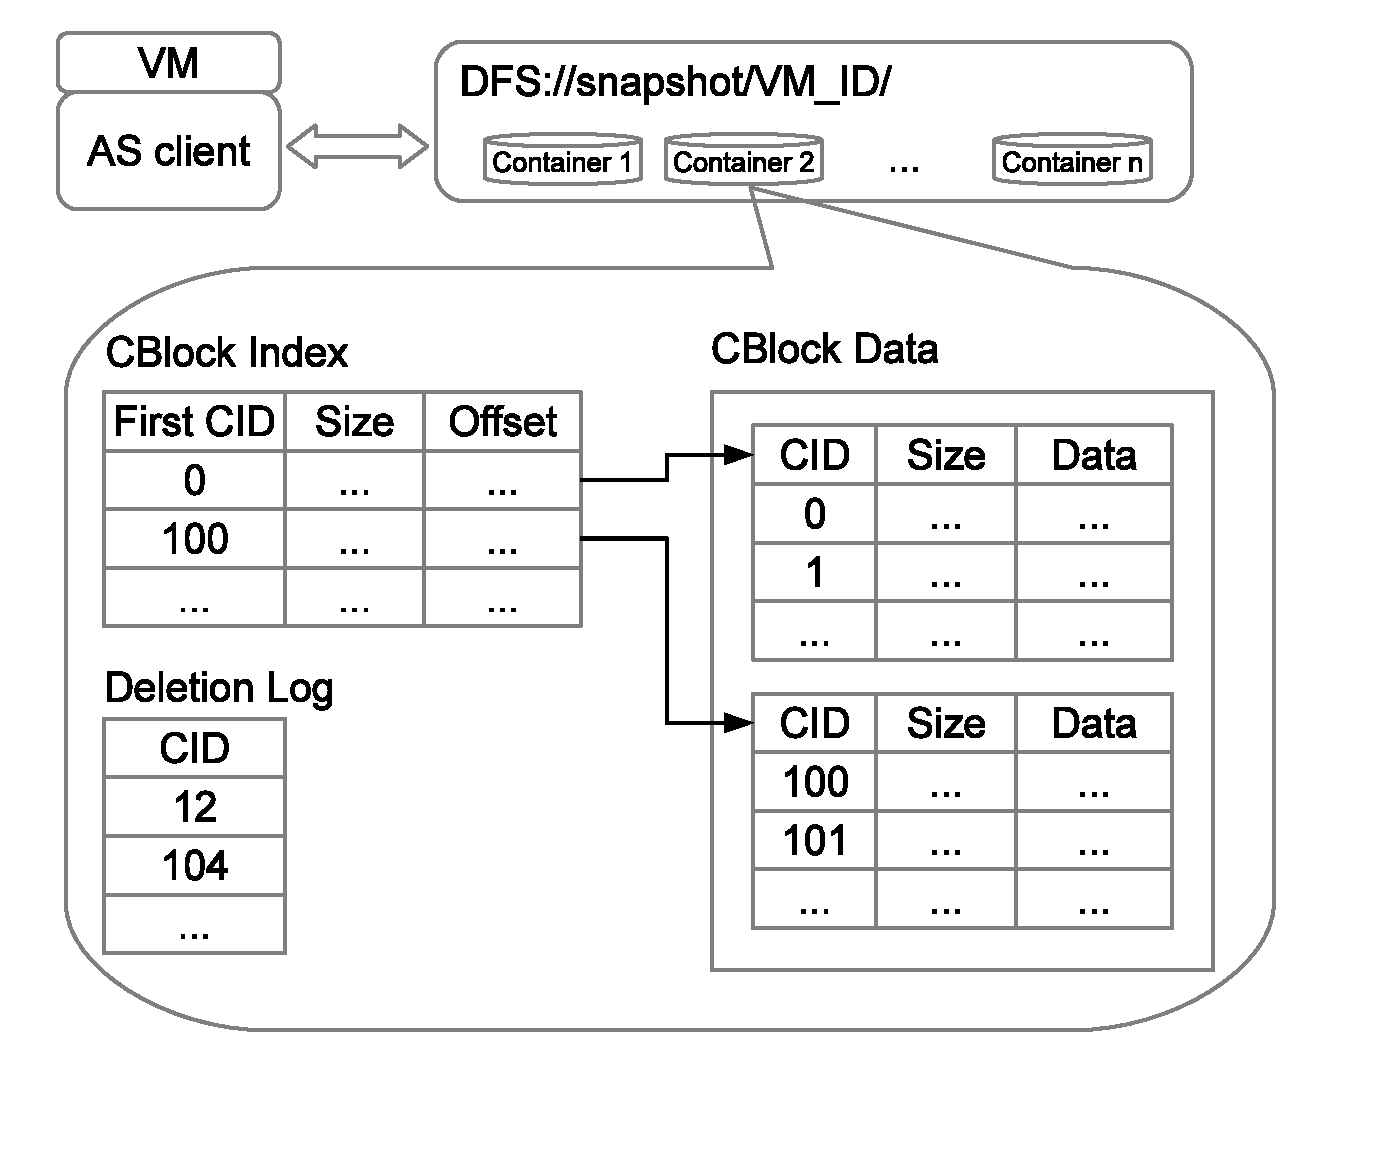
\epsfig{file=images/append_store_arch, width=3.5in}
  \caption{Architecture of Append Store}
  \label{fig:as_arch}
\end{figure}

Append Store supplies three interfaces: {\em get(ref)} accepts a data reference and retrives data, 
{\em put(data)} accepts data and returns a reference to be stored in metadata recipes, 
{\em delete(ref)} 
deletes the data pointed by the reference.
Under the hood, small var-sized data are grouped and stored into larger data containers. Each VM has
its snapshot data stored in its own Append Store, specified by the VM ID. 
We split every Append Store into multiple data containers so that reclaiming the disk space would not 
result in rewriting all the data at the same time.

As shown in Fig.\ref{fig:as_arch}, every data container is represented as three data files in DFS:
the data file holds all the actual data, the index file is responsible for translating data reference
into data locations, and a deletion log file remembers all the deletion requests to the container.

A data reference is composed of two parts: a container ID (2 bytes) and CID (6 bytes).
Append Store assign every piece of data a CID for its internal data referencing. 
When new data is appended, its CID is the current largest CID in that container plus one.
As a result, all the data locations are naturally indexed by this self-incremental CID, 
no extra sorting is needed.

Append Store groups multiple chunk data (i.e., 100) into larger units, called {\em CBlock}.
CBlock is the basic unit for append store's internal read/write/compression.
There is one index entry in the container index corresponding to every CBlock. It keeps the first chunk's CID
in that CBlock, and the CBlock data's size and location.

Using CBlock brings us several advantages: First, the write workload to DFS master is greatly reduced; second, grouping
small chunks gives better compression. Third, reading a CBlock (200 - 600 KB) typically cost the same amount of disk 
seek as reading a 4KB chunk. Finally, this greatly reduces the size of index. Let $m$ be the number of chunks in each
CBlock, then the overall index size is reduced to $1/m$. In our implementation, using $m=100$ reduces the index for
a 1GB container from 10 MB to 100 KB.

\subsection{Operations}
In order to read a chunk data by reference, Append Store client first loads the
container index file specified by the container ID, then search the CBlock index to find the entry that covers the chunk by CID.
After that, it reads the whole CBlock data from DFS, decompress it, seek the exact chunk data specified by CID. 
Finally, the client updates itws internal chunk data cache with the newly loaded contents to anticipate future sequential reads.

Write requests to append store are accumlated. When the number reaches $m$, the AS client forms a CBlock by assigning 
every chunk a CID, compress the CBlock data, and append it to the CBlock data file. Then a new CBlock index entry is appended
to CBlock index.

Append store adopts lazy delete strategy. The deletion requests are appended into every container's deletion log file with the CID of data to be deleted.
CIDs in deletion log are guaranteed to be referenced by nobody and can be safe deleted in future. 
Periodically, snapshot management system asks append store to compact containers in order to reclaim disk space. 
The actual compaction will only take place when the number of deleted items reached $d\%$ of container's capacity. 
During compaction, append store creates a new container (with the same container ID) to replace the 
existing one. This is done by sequentially scan the old container, copying all the chunks that are not 
found in deletion log to the new container, creating new CBlocks and indices. 
However, every chunk's CID is plainly copied rather than re-generated. This does not affect the sorted
order of CIDs in new container, but just leaving holes in CID values. As the result, all data references stored 
in upper level recipes are unaffected, and the data reading process is as efficient as before.

%hard problems

\subsection{Analysis}

Snapshot operation performance analysis:
\begin{table}
    \begin{tabular}{l p{1.5in} l}
        \hline
        Symbol & Description & Measurement \\ \hline
        $N_{seg}$ & Number of segments in the snapshot & ~ \\ [1ex] \\ [-1.5ex]
        $N_{chunk}$ & Number of chunks in one segment & ~ \\ [1ex] \\ [-1.5ex]
        $P_{dirty}$ & Probablity of a segment is dirty & ~ \\ [1ex] \\ [-1.5ex]
        $P_{new}$ & Percentage of new data & ~ \\ [1ex] \\ [-1.5ex]
        $P_{change}$ & Probablity that a chunk is not found in parent snapshot & ~ \\ [1ex] \\ [-1.5ex]
        $P_{in\_PDS}$ & Percentage of chunks in PDS & ~ \\ [1ex] \\ [-1.5ex]
        $T_{scan}$ & Time to scan segment data and caculate content hash & 74 ms \\ [1ex] \\ [-1.5ex]
        $T_{write\_AS}$ & Time of writing a chunk into append store & 0.24 ms \\ [1ex] \\ [-1.5ex]
        $T_{read\_AS}$ & Time of reading a chunk from append store & ~ \\ [1ex] \\ [-1.5ex]
        $T_{read\_chunk}$ & Time of reading a chunk & ~ \\ [1ex] \\ [-1.5ex]
        $T_{check\_PDS}$ & Time of checking PDS & ~ \\ [1ex] \\ [-1.5ex]
        $T_{read\_PDS}$ & Time of reading a chunk data from PDS data store& ~ \\
        \hline
    \end{tabular}
    \caption{List of performance factors}
    \label{tab:as_param}
\end{table}

The overall time of writing a snapshot is:

\begin{dmath}
T_{write} = P_{dirty} * N_{seg} * [max(T_{scan}, T_{read\_AS}) + P_{change} * N_{chunk} * T_{check\_PDS} + P_{new} * N_{chunk} * T_{write\_AS}]
\end{dmath}

The overall time to read a snapshot is:

\begin{dmath}
T_{read} = N_{seg} * {T_{read\_AS} + N_{chunks} * [P_{in\_PDS} * T_{read_PDS} + (1 - P_{in\_PDS}) * T_{read\_chunk}]}
\end{dmath}

Average time of reading a chunk:

\begin{dmath}
T_{read\_chunk} = P_{in\_PDS} * T_{read\_PDS} + (1 - P_{in\_PDS}) * T_{read\_AS}
\end{dmath}

Time of reading append store:

\begin{dmath}
T_{read\_AS} = 0 * P_{in\_cache} + (1 - P_{in\_cache} ) * T_{load\_CBlock}
\end{dmath}
\
%\section{CDS Analysis}
Although locality based data reduction can remove most of the inner-VM duplications,
it's not able to solve the data duplication cross VMs. Different VMs still share large amount
of common data such that their snapshot backups would have a lot of data in common.
Our observations on Aliyun's real VM user data reveals several major sources of cross-VM data duplication:
  \begin{enumerate}
  \item \emph{System-related data}: These data are generated by public third-parties, they are copied/downloaded/installed into VM disks either automatically or manually. Once installed, operations on such data are mostly read only until software updates arrive. For example, data of operating systems, some widely-used software such as Apache and MySQL, and their documations all fall into this category.
  \item \emph{User-generated data}: These data are generated by individual user's behavior, either directly or indirectly. They are much less duplicated than the system-related data, but the zipf-like distribution indicates that a small amount of data in this category could represent most of data duplications.
  \item \emph{Zero-filled data}: Like previous studies [refs here], we've observed that zero-filled data exist pervasively at system wide. They are almost like the spaces and commas in text articles. Under content-based chunking, they were distilled as zero-filled blocks with the maximum allowed length. 
%Zero-filled blocks are mostly generated by user behavior to preserve the space for future data, thus we treat them as a special case of user-generated data.
  \end{enumerate}

Without eliminating the data duplication between VM snapshot backups, storage space is severely wasted when the number of VMs increases.
To address this problem, we developed a technique called \emph{Common Data Set (CDS)} to eliminate data duplication for all three situations above. 
CDS is a public data library that shared by all VM snapshot backups in the cluster, 
which consists of the most popular data blocks in VM snapshot backups. It is generated, 
managed and accessed in an uniform manner by all VMs such that [write some fancy system characteristic stuff here].

\subsection{CDS Size V.S. Coverage}
As a shared data library, we expect CDS to collect almost all the system related data, the most popular user-generated data and the zero-filled data block.
With CDS as a public data reference, each VM's snapshot backup has no need to store its own copies for data that can be found in CDS, instead they can just
store a reference.

The more data we put into CDS, the closer we come to complete deduplication. But in reality we are facing a list of restrictions such like [blabla].
We borrowed the idea of web caching[refs here] to analysis the size of CDS vesus its effectiveness on data reduction.

We let $M$ be the number of machines in a VM cluster, $N$ be the total number of VMs,
$D$ denotes the average size of one VM's snapshot backups, which is near 40 GB in our production clusters.
And let $C_0$, $C_s$ and $C_u$ denote the size of zero-filled block, system-related data and user-generated data in CDS,
then the total size of CDS is represented by $C=C_0+C_s+C_u$.
We let $S_0$, $S_s$ and $S_u$ denote the corresponding average space saving ratio (coverage) relative to $D$ in per VM's snapshot backups,
so the total saving ratio is $S=S_0+S_s+S_u$.

Zero-filled block at maximum length is the first item we need to put into CDS. This is the one and only special data block, 
and because CDS only stores unique data blocks, $C_0$ is almost equal to 0. In practice we found zero-filled blocks account
for near 20\% of total data, so $S_0$ is 20\%.

The rarely modified system-related data are the second to be added to CDS. We have thousands of VMs in each cluster, 
but all these VMs fall into only a few OS types, using a limited selection of software, therefore data duplication in this category
is highly noticable in a global block counting. In particular, most of such data already exist in the VM base images. 
We analyzed VMs running various services from 7 mainstream OS types in our cluster, and found close to 50GB of such data in total. 
Because system-related data don't change frequently, it's safe to expect that for 20 OS variations 
and software updates in 2 years, $C_s$ will not grow to exceed 200 GB.
For each VM, from 2 to 20 GB of data can be reduced in this way, depends on the OS and service type, so on average we estimate
$S_s$ would be no less than 20\%.

The rest of data are user-generated, the total size of such data can be written as $D_u=D-S_0-S_s$, which is 60\% of $D$. 
It follows a zipf-like distribution with $\alpha$ between 0.65 to 0.7. 
Let $T_u$ be the total size of unique data blocks in $D_u$,
in practice we notice that complete deduplication for such data always result in a 2:1 reduction ratio,
, so $T_u=D_u/2$.
Since we collect the most popular user-generated data into CDS, the coverage of CDS on user-generated data
is $(C_u/T_u)^{1-\alpha}$.

The following table lists CDS coverage on user-generated data under different $\alpha$ and $C_u/T_u$.

[a table of coverage with alpha from 0.65-0.70, ratio from 0.002 0.005 0.01 0.02 0.05]

It's obviously that at least 30\% of user-generated data can be reduced in this way, using about 0.02 of $T_u$, or 0.01 of $D_u$.
The size of user-generated data in CDS would be 0.006$D$, with coverage $S_u=0.18D$.

Thus the estimation of CDS coverage is $S=S_0+S_s+S_u=0.58$, with the size of CDS to be no more than $(200 + 0.006*D*N)$ GB.
In a VM cluster of 100 machines, with 25 VMs on each physical machine, the size of CDS is 800 GB in total, or 8 GB per machine.
The total size of CDS index would be 8 GB, which will cost 80 MB memory on each machine. 

\subsection{CDS Access}

\subsection{CDS Management}


%\section{Deletion}
In a mature VM cluster, snapshot deletions are as frequent as snapshot creations.
Our system adopts lazy delete strategy so that all snapshot deletions are scheduled
in the backup time window at midnight. 
Therefore, snapshot deletions must be fast enough to fit in time window and
efficient enough to satisfy our resource constraints.
However, there is no simple solution can achieve these goals with high reliability.
In Aliyun's cloud, we use a {\em fuzzy deletion} method to trade deletion accuracy for
speed and resource usage. This method tolerates a tiny percentage of storage leakage
to make the deletion operation faster and efficient by an order of magnitude,
yet we still adopt an slow but accurate deletion method to fix such leakage in the long-term.
Our hybrid deletion strategy, using fuzzy deletion regularly and accurate deletion periodically,
accomplishs our speed, resource usage and relibility goals very well.

% \subsection{Challenges}
% Contrary to a traditional backup system, a dedupe system shares data among files by default. 
% Reference management is necessary to keep track of chunk usage and reclaim freed space. 
% In addition to scalability and speed, reliability is another challenge for reference management. 
% If a chunk gets freed while it is still referenced by snapshots, data loss occurs and files cannot be restored. 
% On the other hand, if a chunk is referenced when it is actually no longer in use, it causes storage leakage.

% Reference counting, while being simple, suffers from low reliability especially in our distributed environment, 
% because it is vulnerable to lost or repeated updates: when errors occur some chunks maybe updated and some may not. 
% Complicated transaction rollback logic is required to make reference counts consistent. Moreover, 
% there is almost no way to verify if the reference count is correct or not in a large dynamic system. 
% In real deployments, where data integrity and recoverability directly affect product reputation, simple reference counting is unsatisfactory.

% Mark-and-sweep is generally a better solution. During the mark phase, all snapshot recipes are traversed so as to mark the used chunks. 
% In the sweep phase all chunks are swept and unmarked chunks are reclaimed. 
% This approach is very resilient to errors: at any time the process can simply be restarted with no negative side effects. 
% Scalability, however, is an issue. {\em needs to explain its resource usage}


\subsection{Approximate Deletion}
\begin{figure}[htbp]
  \centering
  \epsfig{file=images/deletion.png, width=3.5in}
  \caption{Approximate deletion}
  \label{fig:deletion_flow}
\end{figure}

We design approximate deletion to fast identify unused data in the append store.
Instead of scanning the whold append store, it uses a Bloom filter to check 
if a data are still referenced by living snapshots. However, there is a small false-positive probility which
would indetify unused data as in use, i.e., storage leakage.
The following steps would take place during an approximate deletion:

\begin{enumerate}
\item {\bf Creating Bloom filter} Scan all the living snapshot recipess and their segment recipes,
for every reference pointing to append store, add it to the Bloom filter.
\item {\bf Check existance} For every data reference in the deleted snapshot recipe and its segment recipes,
check the existance of that data reference in Bloom filter. If not found, it is safe to delete that piece of data from append store
because no living snapshots has referenced it.
\end{enumerate}

The overall time of running a approximate deletion for one snapshot deletion would be scanning
all the living snapshots and deleted snapshots, since operations on the in-memory Bloom filter can be done in
parallel and is much faster than loading recipes from DFS:
\begin{equation}
T = (N_{SS} + 1) * T_{scan\_recipes}
\end{equation}
 
Using the example and analysis in previous section, this approximate deletion can be done in 5 minutes. 
Memory usage of the Bloom filter depends on its false-positive probility $P_{bl}$,
when set $P_{bl}$ to 0.01, the memory footprint of approximate deletion is about 15 MB.

The design goal of approximate deletion is to reduce the frequency of running accurate deletion.
For one VM's snapshots, let $D_{leakage}$ be the amount of storage leakage, $D_{del}$ be the average amount of data
to be deleted in one snapshot deletion, 
then we have:
\begin{equation}
D_{leakage} = N_{approximate} * P_{bl} * D_{del}
\end{equation}
where $N_{approximate}$ is the number of runs of approximate deletion. 
An accurate deletion is triggered to fix the storage leakage
when $D_{leakage}/D_{del}$ is accmulated to exceed certain threshold $T$:
\begin{equation}
D_{leakage} / D_{del} = N_{approximate} * P_{bl} > T \Rightarrow N_{approximate} > T/P_{bl}
\end{equation}
Therefore, when $P_{bl} = 0.01$ and $T=1$, 
there would be a run of accurate deletion for every $T/P_{bl} = 100$ runs of approximate deletion.
On a machine that hosts 20 VMs and each VM deletes snapshot daily, there would be less than
one accurate deletion scheduled per day.

\subsection{Accurate Deletion}
Our accurate deletion uses mark-and-sweep to find all the unused chunks in a VM's append store.
The following steps would take place during an accurate deletion:

\begin{enumerate}
\item Scan all the containers. For each container, extract full list of existing data references and allocate a bitmap. 
(Notice this list is self sorted.)
\item Scan all the snapshot recipes and segment recipes. For every data reference pointing to append store,
find it in the above lists and mark the corresponding position in bitmaps.
\item Scan the bitmaps, for every bit that are not marked, tell append store the corresponding data reference can be deleted.
\end{enumerate}

Although accurate deletion guarantees reliability and correctness, its speed and resource usage are big problems to our VM cloud.
Let $T_{scan\_AS}$ be the time to scan the VM's append store, $T_{scan\_recipes}$ be the time to scan one snapshot recipe
and its segment recipes, $T_{mark}$ be the time of finding a data reference in the list and mark bitmap, 
$N_{SS}$ be the number of snapshots and $N_c$ be the number of chunks in one snapshot.
The overall time of running an accurate deletion for one VM is:
\begin{equation}
T = T_{scan\_AS} + N_{SS} * T_{scan\_recipes} + N_{SS} * N_c * T_{mark}
\end{equation}

For a virtual disk that has 10 snapshots, 50 GB of data in the append store, $T_{scan\_AS}$ would have cost half an hour already.
In addition, scanning recipes of 10 snapshots cost another 5 minutes.
Furthermore, maintaining the full lists of data references and bitmaps costs about 100 MB of memory. Having tens of VMs
co-lived in one physical machine and deleting snapshot on a daily basis, 
it's infeasible to run accurate deletion as frequent as snapshot deletions.

\subsection{Discussion}

%\subsection{Storage Space and Impact on Fault Tolerance}
 
\begin{figure}
    \centering
    \subfigure[Sharing of data under VM-centric dedup model]
    {
        \includegraphics[width=3in]{images/share_vc}
        \label{fig:share_vc}
    }
    \\
    \subfigure[Sharing of data under VM-oblivious dedup model]
    {
        \includegraphics[width=3in]{images/share_vo}
        \label{fig:share_vo}
    }
    \caption{Bipartite association of VMs and file blocks under VO and VC approaches}
    \label{fig:share}
\end{figure}

The replication degree of the backup storage 
is $r$ for regular file blocks and $r=3$ is a typical setting in the distributed
file system~\cite{Hadoop,GFS}.
In the VC approach, a special replica degree $r_c$ used for PDS blocks where $r_c>r$. 
The storage cost for VO with full deduplication is $c_u *r$ and for VC, it is
$ k*r_c  + (c_u-k)*r$. Thus The storage cost ratio of $VC$ over $VO$ is 
\[
\sigma \frac{r_c}{r} + 1-\sigma
\]
Since $sigma$ is small,  term $\sigma \frac{r_c}{r}$ is small in the above expression.  
Thus the impact on storage increase is very small when we choose a large $\frac{r_c}{r}$ ratio. 
For example, $\frac{r_c}{r}=2$. 


%In our experiment with Alibaba data, the ratio $\sigma$ 
%is 162. Thus allocation of extra replicas for PDS only introduces a small amount of extra space
%cost.  Figure~\ref{fig:storagePDS} shows the storage cost ratio of VC and VO when 
%$r$=3, and $r_c$ varies from 3 to 10.
%The result shows that the storage cost for adding extra replication for PDS
%is insignificant.

Next we  assess  the impact of losing $d$ machines 
to the the VC and VO approaches.  
A large $\frac{r_c}{r}$ ratio can have a positive impact on full availability of snapshot blocks.


\comments{
For each rank $i$ block which appears $C_i$ times  among $V$ virtual machines.
Assigning this block to virtual machines can be viewed as a classical ball-bin assignment
approximated by a Poisson distribution. Namely the virtual machines that share this block
is approximated as $1 -  e^{C_i/V}$.
Thus the average number of VMs that share a block is:
\[
(1-\delta) + \delta \sum_1^{u_b} \frac{1 -  e^{C_i/V}}{u_b}.
\]
Any failure of a block would impact the above number of virtual machines.
In VO, the number of VMs that share a block is:
\[
\sum_1^{u_b'} \frac{1 -  e^{C_i'/V}}{u_b'}.
\]

Next we discuss how a failure of $d$ machines impacts the VM snapshots in VC.
When $d<r$, there is no loss of data in the snapshot storage.
When $r_c> d \ge r$, some of data blocks in the storage are lost, and we compute the number of VMs that could
suffer the loss of their snapshots.
When $d \ge r_c$, some of PDS blocks are affected.
In VC, the blocks in PDS are stored in a container manner (superblock), and they are shared by many VMs.
The number of data containers stored with replication degree $r$ for
referenced by each VM is:
\[
N_1= \frac{b}{v*s} (1-\delta) +b/(v*s)\delta (1 -  (\frac{k}{b_u})^{1-\alpha}).
\]
The number of PDS data containers stored with replication degree $r_c$ for
referenced by each VM is:
\[
N_2= \frac{b}{v*s}\delta (\frac{k}{b_u})^{1-\alpha}.
\]
}



%Thus the number of VMs using a block =    $(1-s_c)  + s_c *L$.
%In characterizing the reliability of VM backups in our model, 
%we consider the likely hood that a file system block fails,
%given some number of storage machine failures. 
%Every time a filesystem block fails,
%we say that we have lost data for that virtual machine, so it is no longer
%available. 
%In reality it may be only one snapshot that is affected, but it is the user
%who must decide which snapshots are important, so we consider the worst case. 
We use filesystem blocks rather than a deduplication
data chunk as our unit of failure because the DFS keeps
filesystem blocks as its base unit of storage.
% (in our case there are 
%16384 blocks in a filesytem block on average, with 4KB block size and 
%a 64MB block size).
To  compute the full availability of all snapshots of a VM, we derive
the probablity of losing a snapshot file block of a VM by
estimating the number of file system blocks per VM in each approach.
As illustrated in Figure~\ref{fig:share},
we build a bipartite graph representing the association from unique file system blocks
to their corresponding VMs in each approach. An association edge is  drawn  from a file block  to a VM 
if this block is used by this VM. 
For VC, each VM has an 
average number of $N_1$ file system blocks for non-PDS data. 
It also refers  an average of   $N_2$ file system blocks for PDS data. 
For VO, each VM has an average  of  $N_o$ file system blocks
and let $V_o$ be the average number of VMs shared by each file system block.
%Figure~\ref{fig:shared} illustates the bipartite association.

In VC, each non-PDS file system block is associated with one VM
 and  PDS file system blocks are
shared by an average of $V_c$ VMs. Let $s$ be the average number of chunks per file block. Thus, 
\[
V *p*N_1 *s  = C_u (1-\sigma)\; \mbox{ and } \; 
V *p*N_2 *s  = C_u \sigma *V_c
\]
For the VO approach, 
\[
V *p*N_o *s  = C_u  V_o.
\]

Since each file block (with default size $64MB$) contains many chunks (on average 4KB),
each file block contains the hot low-level chunks shared by many VMs, and it also contains
rare chunks which are not shared.  From the about equations.
\[
\frac{N_1}{N_o}=  \frac{1-\sigma}{V_o}<1.
\] 
Thus when there is a failure in file blocks with replication degree $r$
and there is no failure for PDS data with more replicas,   a VM in
the VC approach has a lower chance to lose a snapshot than the VO approach because
$N_1<N_o$. 
Figure~\ref{fig:fsb-links} shows the number of VMs sharing by each file block.
%In our experiment, we find that $V_o \approx 0.2 V$ when backing up VMs one by one.
We can observe that $N_1 +N_2 < N_o$. 
This is likely because the PDS FSBs tightly pack data used by many VMs, 
which decreases the overall number of FSBs required to backup a VM.
If  the backup for multiple VMs is conducted concurrently, there would be more
VMs shared  by each file block on average. Therefore,
even when there is a loss of a PDS block, the VC approach tolerates the fault better.

%Figure~\ref{fig:fsb-links} shows the average number of VMs sharing a
%filesystem block (FSB) as VMs are added. Though we don't expect the linear trend to continue indefinitely for
%much larger datasets, it should continue to increase, which has important implications
%on VM backup availability in the precense of failures. Below we show the
%significant impact the number of links has on VM backup reliability.

\comments{%dropping block links bec. we don't use it elsewhere
\begin{figure}[htbp]
  \centering
  %\includegraphics[scale=.45,natwidth=511,natheight=276]{vo_links}
	\begin{tikzpicture}
		\begin{axis}[
		%title={VO Block links},
		xlabel={Number of VMs added},
		ylabel={Avg. links to a chunk},
		%extra y ticks={4.5,5.5,6.5} %because it only shows 4,5,6,7
		legend pos=south east
		]
		\addplot table[x=VMs,y=Measured] {figures/vo_links.txt};
		\addplot table[x=VMs,y=Theoretical] {figures/vo_links.txt};
		\legend{Measured,Theoretical};
		\end{axis}
	\end{tikzpicture}
  \caption{Average number of VMs sharing a data chunk in the global index}
  \label{fig:vo-links}
\end{figure}
}

\begin{figure}[htbp]
  \centering
	\begin{tikzpicture}
		\begin{axis}[
                width=\linewidth,
                height=0.6\linewidth,
		%title={VO FSB links},
		xlabel={Number of VMs},
		ylabel={Avg. Num. VMs sharing FSB},
                cycle list name=mline,
                xmin=0,
                ymin=0,
                xmax=106,
		%extra y ticks={4.5,5.5,6.5} %to show extra ticks
		legend pos=north west
		]
                \addplot table[x=VMs,y=FSBLinks] {figures/vo_fsb_links_105.txt};
		\addplot table[x=VMs,y=cdslinks] {figures/cds_links_105.txt};
                \legend{VO, PDS in VC};
		\end{axis}
	\end{tikzpicture}
  \caption{Measured Average number of VMs sharing a 64MB FSB with global dedup (VO), and in a 2\% PDS for VC.}
  \label{fig:fsb-links}
\end{figure}



\begin{figure}[htbp]
  \centering
	\begin{tikzpicture}
		\begin{axis}[
		%title={VO VM links},
                width=\linewidth,
                height=0.6\linewidth,
		xlabel={Number of VMs},
		ylabel={Avg. Num. FSBs used by VM},
                xmin=0,
                ymin=0,
                xmax=106,
		%extra y ticks={4.5,5.5,6.5} %to show extra ticks
		legend pos=south west
		]
                \addplot[blue,mark=none] table[x=VMs,y=No] {figures/vo_vm_links_105.txt};
                \addplot[red,dotted,mark=none] table[x=VMs,y expr=\thisrow{N1}+\thisrow{N2}] {figures/vc_vm_links_105.txt};
                \addplot[red,dashdotted] table[x=VMs,y=N1] {figures/vc_vm_links_105.txt};
                \addplot[red,densely dashed,mark=none] table[x=VMs,y=N2] {figures/vc_vm_links_105.txt};
                \legend{$N_o$, $N_1+N_2$, $N_1$, $N_2$};
		\end{axis}
	\end{tikzpicture}
  \caption{Measured Average number of 64MB FSBs used by a single VM. For VC both the number of PDS and Non-PDS FSBs used are shown.}
  \label{fig:vm-links}
\end{figure}


 The full snapshot availability of a VM is estimated as follows with parameters $N_1$, $N_2$, and $N_o$.
%the likelyhood that there is no  data loss for all its file blocks.  
With replication degree $r$, the availability of a file block is the probability that  
all of its replicas do not appear in any group of $d$ failed machines. 
Namely, $1-\binom{d}{r}/ \binom{p}{r}$. 
The snapshot availability of a VM  in the VO approach is
\[ 
(1-\frac{ \binom{d}{r}} { \binom{p}{r} })^{N_o}. 
\]
%This can be seen in Figure~\ref{fig:fsb-availability} for a 100 machine cluster for 3 different replication factors.
When there are $r \le d<r_c$ machines failed,  there is no PDS data loss and  
%a file block failure depends on if all replicas of this container reside in the failed machines.
the full snapshot availability of a VM in the VC approach is 
and is
\[
(1-\frac{\binom{d}{r}} { \binom{p}{r} })^{N_1}.
\]
%\begin{multline}
%= Probability (\mbox{ There is no file block loss in this VM}) \\
%= Probability(\mbox{ A file block has file data loss})^{N_1}\\
%= (1- Probability (\mbox{all replicas of its block fail}))^{N_1}\\
%\end{multline}
%\end{split}
Since $N_1 <N_o$, the VC approach has a higher availability of VM snapshots than VO.

When $r_c \leq d$, both non-PDS and PDS file blocks in VC can have a loss.
The full snapshot availability of  a VM in the VC approach is
\[
(1-\frac{ \binom{d}{r}} { \binom{p}{r} })^{N_1} 
*
(1-\frac{ \binom{d}{r_c}} { \binom{p}{r_c} })^{N_2}.
\]
Both conditions $N_1+N_2 <N_o$ 
and  $1-\frac{ \binom{d}{r}} { \binom{p}{r} }
< 1-\frac{ \binom{d}{r_c}} { \binom{p}{r_c} }$
support the higher availability of VC.
%= Probability(\mbox{ No non-PDS file block loss})^{N_1}
%Probability(\mbox{ No PDS file block loss})^{N_2}\\
%\begin{multline}
%\end{split}
%\end{multline}




%By comparison, the probability that a VM has data loss is close to
%1 once  there are  $d \ge r$ failed machines. That is because there are more data blocks
%shared among VMs. Any failure of these blocks causes many more VMs to fail.


\comments{
We take the likelyhood of VM failure to be the same as the likelyhood of chunk failure,
so
\[
    P_{VMfailure}=\frac{\binom{d}{r}}{\binom{p}{r}}
\]

Since both in the PDS and in the VO approach a single filesystem chunk may be used by many VMs,
we must multiply the block failure ratio by the number of outgoing links for the block to get
the expected impact on the system.
\[
    E_{VMfailure}=L\frac{\binom{d}{r}}{\binom{p}{r}}
\]

in our current testbed we have measured the average number of links per chunk
(Figure~\ref{vo-links}) and number of links per Filesystem Block (FSB)
(Figure~\ref{fig:fsb-links}) in our dataset. For the complete dataset, we also
found the average number of links to PDS chunks, which was \~19 using a 2\%
PDS. From Figure~\ref{fig:fsb-links} you can see that as you add VMs, the
average number of links to a chunk increases linearly for our dataset. We
expect that this trend will level out with larger datasets, but should continue
to increase at a slower rate.  For the VC model, we have to consider both PDS
chunks and non-PDS chunks. In the VO model all data is shared, but in VC only
the PDS data is shared, but at a much higher rate. This gives a strong
advantage to VC, in that for a large percent of the data (95-99\%), there is
only one VM pointing to each non-PDS chunk. You can see the increase in
reliability in Figure~\ref{fig:vm-availability}.
\begin{table}
    \begin{tabular}{|l|lll|}
    \hline
    \multirow{2}{*}{Nodes Failed}   & \multicolumn{3}{c|}{Availability(\%)}\\
                                    & $R=3$ & $R=4$ & $R=5$\\
    \hline
    1           &  100      & 100       & 100\\
    2           & 100       & 100       & 100\\
    3          & 99.999     & 100       & 100\\
    5          & 99.993     & 99.9999   & 99.999998\\
    10          & 99.926    & 99.995    & 99.999\\
    20          & 99.295    & 99.876    & 99.979\\
    \hline
    \end{tabular}
    \caption{Availability in a 100 machine cluster of a single FSB with different replication factors}
    \label{tab:fsb-availability}
\end{table}

}
\comments{
\begin{figure}[htbp]
  \centering
    \begin{tikzpicture}
            \begin{axis}[
                width=\linewidth,
                height=0.6\linewidth,
            %title={FSB Availability},
            cycle list name=mline,
            xlabel={Number of Machines Failed},
            ylabel={Availability of Single FSB (\%)},
            extra y ticks={99.9}, %to add extra ticks
            mark options=solid,
            legend pos=south west,
            %legend columns=2,
            %legend style={
            %    at={(0.5,-0.2)},
            %anchor=north}
            ]
            \addplot table[x=NodesFailed,y=Availability5] {figures/fsb_availability.txt};
            \addplot table[x=NodesFailed,y=Availability4] {figures/fsb_availability.txt};
            \addplot table[x=NodesFailed,y=Availability3] {figures/fsb_availability.txt};
            \legend{$R=5$,$R=4$,$R=3$};
            \end{axis}
    \end{tikzpicture}
    \caption{Availability of Individual FSBs in 100 Machine Cluster with different replication factors.}
  \label{fig:fsb-availability}
\end{figure}
}






%\section{Experiments}
Our main test-bed is an cluster of 6 machines,
each of which is equiped with a 8-core AMD FX-8120 at 3.1 GHz
with 16 GB RAM, running Linux. 
A distributed file system (QFS) runs

We used two main data sets for testing. Our synthetic
data set consists of multiple 3 GB files, each with globally
unique data segments. Our second data set consists
of virtual machine images, which are a very common
real-world enterprise use-case, that takes advantage
of deduplication. We use a VMware “gold” disk image
(VM0), hosting a Microsoft Windows XP installation,
and created three additional versions of it (VM1, VM2,
and VM3), each with incremental changes: VM1 is VM0
with all Microsoft updates and service packs, VM2 is
\section{Conclusion}
In this paper, a empirical study using Aliyun's real user VM data traces is conducted. 
We present a number of observations and insights on the data duplication
in VM snapshot backups. We describe
in detail the patterns of VM access, VM snapshot duplication, locality reduction, and
the dintinct difference between OS and user generated data.
We hope this will facilitate future designs of cloud storage for VMs.

\bibliographystyle{abbrv}
\bibliography{library}
\end{document}
